% (C) Brett Klamer - MIT - http://opensource.org/licenses/MIT
% Please contact me if you find any errors or make improvements
% Contact details at brettklamer.com

\documentclass[11pt,letterpaper,english,oneside]{article} % article class is a standard class
%==============================================================================
%Load Packages
%==============================================================================
\usepackage[left=1in,right=1in,top=1in,bottom=1in]{geometry} % easy page margins
\usepackage[utf8]{inputenc} % editor uses utf-8 encoding
\usepackage[T1]{fontenc} % T1 font pdf output
\usepackage{lmodern} % Latin modern roman font
\usepackage{bm, bbm} % bold and blackboard bold math symbols
\usepackage{amsmath, amsfonts, amssymb, amsthm} % math packages
\usepackage[final]{microtype} % better microtypography
\usepackage{graphicx} % for easier grahics handling
\usepackage[hidelinks, colorlinks=true, linkcolor = blue, urlcolor = blue]{hyperref} % to create hyperlinks
\usepackage{float} % tells floats to stay [H]ere!
\usepackage{enumitem} % nice lists
\usepackage{fancyhdr} % nice headers
\usepackage{caption}  % to control figure and table captions
\usepackage{booktabs} % to create nice tables

%==============================================================================
% Enter title and authors here
%==============================================================================
\author{Kshitiz Parihar$^1$, 
Jonathan Nukpezah$^2$, 
Daniel V Iwamoto$^3$, 
Katrina Cruz$^3$, 
Fitzroy J Byfield$^3$, \\
LiKang Chin$^3$, 
Maria E Murray$^3$, 
Melissa G Mendez$^3$, 
Anne S van Oosten$^3$, 
Anne Herrmann$^3$, \\
Elisabeth E Charrier$^3$, 
Peter A Galie$^3$, 
Megan Donlick$^3$, 
Tongkeun Lee$^3$, \\
Paul A Janmey$^{2,3,4}$, 
Ravi Radhakrishnan$^{1,2}$
}
\title{Tissue-dependent mechanosensing by cells derived from human tumors}

\date{%
    $^1$Department of Chemical and Biomolecular Engineering, School of Engineering and Applied Science, University of Pennsylvania, Philadelphia, PA, USA \\
    $^2$Department of Bioengineering, School of Engineering and Applied Science, University of Pennsylvania, Philadelphia, PA, USA \\
    $^3$Institute for Medicine and Engineering, University of Pennsylvania, Philadelphia, PA, USA \\
    $^4$Department of Physiology, Perelman School of Medicine, University of Pennsylvania, Philadelphia, PA, USA \\
}

%==============================================================================
% Put title and author in PDF properties
%==============================================================================
\makeatletter % change interpretation of @
\hypersetup{pdftitle={\@title},pdfauthor={\@author}}

%==============================================================================
% Header settings
%==============================================================================
\pagestyle{fancy} % turns on fancy header styles
\fancyhf{} % clear all header and footer fields
\makeatletter
\makeatother
\rhead{\thepage} % right header
\setlength{\headheight}{13.6pt} % fixes minor warning
\makeatother % change back interpretation of @

%==============================================================================
% List spacing
%==============================================================================
\setlist[itemize]{parsep=0em} % fix itemize spacing
\setlist[enumerate]{parsep=0em} % fix enumerate spacing

%==============================================================================
% Float spacing (changes spacing of tables, graphs, etc)
%==============================================================================
%\setlength{\textfloatsep}{3pt}
%\setlength{\intextsep}{3pt}

%==============================================================================
% My additions
%==============================================================================
\usepackage{changepage} % for the adjustwidth environment
% commented out
%\captionsetup{width=0.9\textwidth, justification = raggedright}


\begin{document}

\renewcommand{\figurename}{Supplementary Figure}

\maketitle

\begin{table}[!h]
\centering
\caption{\label{tab:count-area}Number of spread area, aspect ratio, and circularity measurements for each cell line-substrate combination.}
\centering
\begin{tabular}[t]{lccccccc}
\toprule
  & 30kPa Coll & 30kPa FN & 500Pa Coll & 500Pa FN & Glass & HA Coll & HA FN\\
\midrule
SK-MEL-2 & 100 & 100 & 101 & 100 & 100 & 101 & 100\\
A375 & 100 & 100 & 101 & 100 & 100 & 100 & 100\\
WM266-4 & 100 & 100 & 100 & 100 & 100 & 100 & 100\\
MeWo & 50 & 50 & 100 & 96 & 100 & 100 & 80\\
RWPE-1(N) & 102 & 103 & 100 & 103 & 100 & 101 & 101\\
22Rv1 & 99 & 100 & 99 & 81 & 103 & 103 & 98\\
LnCaP & 41 & 49 & 34 & 59 & 90 & 32 & 46\\
DU145 & 77 & 99 & 67 & 101 & 81 & 102 & 103\\
PC-3 & 101 & 100 & 100 & 90 & 100 & 100 & 40\\
hTERT-HPNE(N) & 94 & 100 & 106 & 97 & 100 & 77 & 76\\
Panc-1 & 100 & 102 & 72 & 21 & 101 & 103 & 105\\
Capan-1 & 105 & 100 & 102 & 100 & 101 & 101 & 100\\
SKOV-3 & 108 & 101 & 82 & 104 & 102 & 100 & 92\\
Caov-3 & 85 & 34 & 37 & 16 & 81 & 59 & 43\\
OVCAR-3 & 100 & 86 & 94 & 89 & 90 & 100 & 97\\
NL20(N) & 168 & 257 & 247 & 284 & 248 & 126 & 150\\
NCI-H2126 & 100 & 100 & 100 & 100 & 100 & 100 & 100\\
NCI-H2087 & 100 & 100 & 100 & 100 & 100 & 100 & 100\\
HCT116 & 100 & 100 & 107 & 101 & 101 & 100 & 100\\
HT29 & 82 & 55 & 93 & 40 & 165 & 95 & 49\\
SW480 & 100 & 100 & 100 & 100 & 100 & 100 & 100\\
SW620 & 101 & 100 & 100 & 100 & 101 & 100 & 100\\
hTERT-HME1(N) & 100 & 100 & 101 & 100 & 100 & 74 & 51\\
MCF10A(N) & 100 & 100 & 100 & 100 & 91 & 88 & 62\\
T-47D & 100 & 100 & 100 & 86 & 100 & 84 & 97\\
MCF7 & 100 & 68 & 100 & 82 & 100 & 45 & 29\\
MDA-MB-231 & 121 & 218 & 145 & 164 & 193 & 77 & 160\\
HCC1937 & 100 & 100 & 100 & 100 & 100 & 100 & 100\\
U-87 & 101 & 101 & 102 & 100 & 101 & 101 & 100\\
T98G & 100 & 101 & 100 & 101 & 101 & 100 & 101\\
\bottomrule
\end{tabular}
\end{table}


\begin{table}[!h]
\centering
\caption{Number of measurements of cell stiffness for each cell line-substrate combination.
  \label{tab:count- cell_stiffness}}
\centering
\begin{tabular}[t]{lccccccc}
\toprule
  & 30kPa Coll & 30kPa FN & 500Pa Coll & 500Pa FN & Glass & HA Coll & HA FN\\
\midrule
SK-MEL-2 & 45 & 44 & 43 & 47 & 45 & 50 & 43\\
A375 & 45 & 30 & 39 & 44 & 45 & 42 & 48\\
WM266-4 & 63 & 44 & 42 & 41 & 44 & 41 & 48\\
MeWo & 29 & 31 & 30 & 33 & 30 & 33 & 30\\
RWPE-1(N) & 30 & 36 & 43 & 48 & 67 & 45 & 30\\
22Rv1 & 30 & 30 & 45 & 30 & 45 & 42 & 30\\
LnCaP & 29 & 15 & 27 & 12 & 48 & NA & 38\\
DU145 & 47 & 44 & 51 & 51 & 49 & 41 & 50\\
PC-3 & 45 & 39 & 35 & 29 & 45 & 30 & 28\\
hTERT-HPNE(N) & 45 & 49 & 50 & 42 & 45 & 45 & 45\\
Panc-1 & 36 & 43 & 30 & 39 & 45 & 43 & 44\\
Capan-1 & 44 & 31 & 29 & 27 & 33 & 32 & 29\\
SKOV-3 & 44 & 39 & 29 & 27 & 28 & 30 & 26\\
Caov-3 & 44 & 45 & 44 & 45 & 45 & 44 & 28\\
OVCAR-3 & 45 & 44 & 45 & 44 & 46 & 47 & 45\\
NL20(N) & 30 & 30 & 30 & 33 & 33 & 30 & 32\\
NCI-H2126 & 30 & 45 & 29 & 30 & 30 & 30 & 30\\
NCI-H2087 & 30 & 29 & 32 & 30 & 30 & 51 & 30\\
HCT116 & 65 & 45 & 49 & 42 & 67 & 66 & 54\\
HT29 & 45 & 39 & 45 & 32 & 45 & 45 & 48\\
SW480 & 44 & 53 & 45 & 59 & 63 & 45 & 45\\
SW620 & 31 & 29 & 45 & 32 & 31 & 30 & 48\\
hTERT-HME1(N) & 45 & 45 & 30 & 47 & 47 & 27 & 45\\
MCF10A(N) & 45 & 44 & 44 & 45 & 60 & 45 & 45\\
T-47D & 48 & 44 & 45 & 45 & 48 & 39 & 42\\
MCF7 & 52 & 42 & 47 & 42 & 29 & 45 & 45\\
MDA-MB-231 & 45 & 45 & 30 & 30 & 32 & 30 & 45\\
HCC1937 & 42 & 30 & 45 & 44 & 39 & 42 & 42\\
U-87 & 51 & 35 & 59 & 54 & 72 & 54 & 45\\
T98G & 63 & 64 & 59 & 61 & 61 & 57 & 56\\
\bottomrule
\end{tabular}
\end{table}


\begin{table}[!h]
\centering
\caption{\label{tab:count-motility}Number of cell speed measurements for each cell line-substrate combination.}
\centering
\begin{tabular}[t]{lccccccc}
\toprule
  & 30kPa Coll & 30kPa FN & 500Pa Coll & 500Pa FN & Glass & HA Coll & HA FN\\
\midrule
SK-MEL-2 & 71 & 72 & 61 & 141 & 129 & 70 & 68\\
A375 & 50 & 50 & 50 & 50 & 51 & 52 & 51\\
WM266-4 & 41 & 46 & 54 & 51 & 50 & 51 & 51\\
MeWo & 176 & 58 & 255 & 53 & 159 & 30 & 72\\
RWPE-1(N) & 119 & 109 & 114 & 102 & 66 & 108 & 105\\
22Rv1 & 36 & 42 & 50 & 45 & 48 & 50 & 56\\
LnCaP & 48 & 50 & 29 & 50 & 50 & 48 & 53\\
DU145 & 41 & 11 & 27 & 43 & 32 & 50 & 39\\
PC-3 & 13 & 21 & 13 & 99 & 101 & 24 & 14\\
hTERT-HPNE(N) & 55 & 52 & 51 & 51 & 52 & 47 & 50\\
Panc-1 & 45 & 44 & 33 & 8 & 57 & 62 & 55\\
Capan-1 & 52 & 46 & 79 & 17 & 56 & 53 & 30\\
SKOV-3 & 33 & 26 & 39 & 49 & 51 & 62 & 44\\
OVCAR-3 & 29 & 52 & 49 & 53 & 58 & 51 & 50\\
NL20(N) & 61 & 70 & 54 & 67 & 26 & 45 & 44\\
NCI-H2126 & 51 & 56 & 72 & 75 & 85 & 56 & 103\\
NCI-H2087 & 87 & 27 & 103 & 114 & 104 & 93 & 69\\
HCT116 & 47 & 36 & 44 & 9 & 70 & 26 & 23\\
HT29 & 50 & 36 & 57 & 15 & 50 & 50 & 50\\
SW480 & 56 & 50 & 55 & 83 & 0 & 40 & 65\\
SW620 & 25 & 25 & 51 & 51 & 25 & 51 & 36\\
hTERT-HME1(N) & 51 & 29 & 50 & 54 & 52 & 20 & 32\\
MCF10A(N) & 50 & 50 & 50 & 60 & 50 & 50 & 52\\
T-47D & 30 & 56 & 31 & 46 & 14 & 81 & 27\\
MCF7 & 22 & 15 & 37 & 3 & 50 & 50 & 36\\
MDA-MB-231 & 27 & 25 & 30 & 29 & 34 & 12 & 26\\
HCC1937 & 51 & 49 & 54 & 50 & 50 & 53 & 48\\
U-87 & 59 & 54 & 52 & 102 & 70 & 58 & 47\\
T98G & 74 & 82 & 123 & 94 & 62 & 75 & 86\\
\bottomrule
\end{tabular}
\end{table}


\clearpage
\begin{figure}
    \centering
    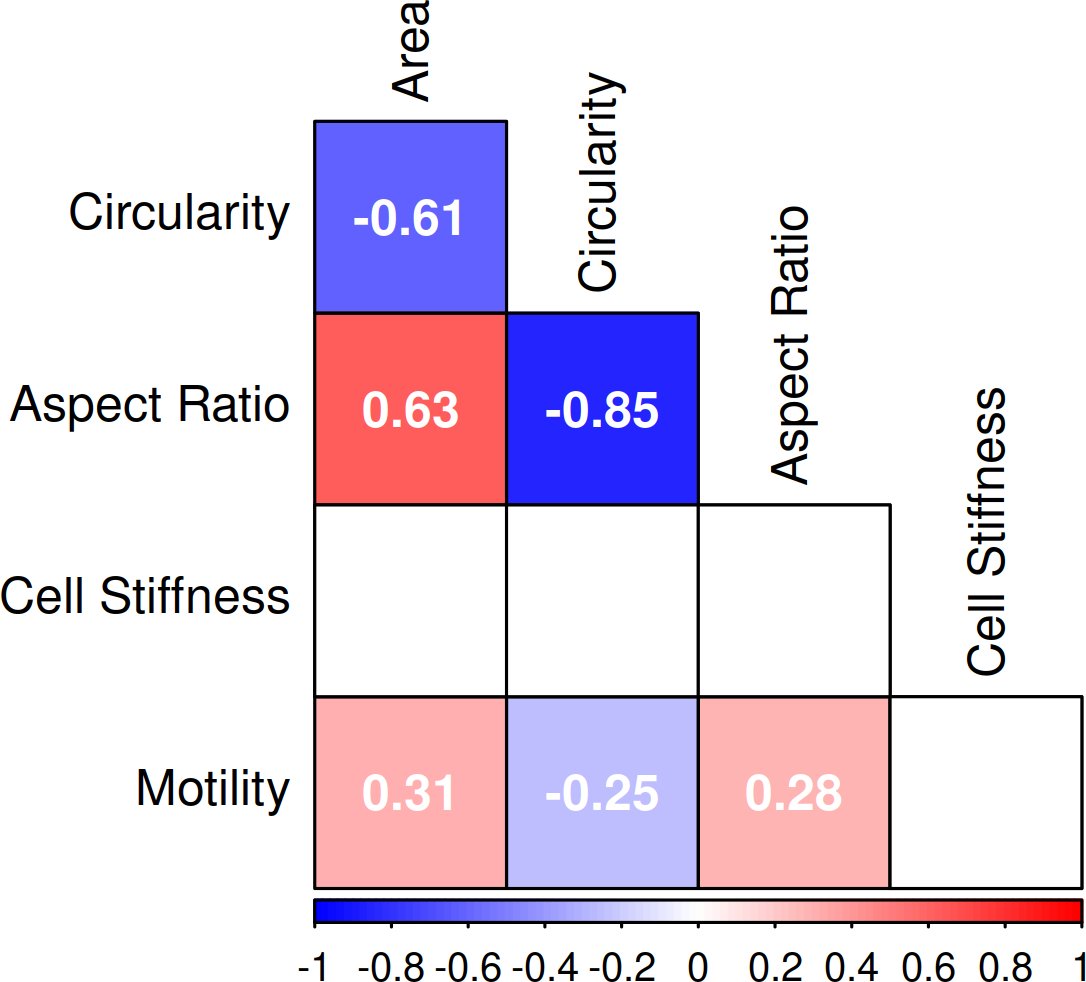
\includegraphics[scale=0.8]{../Figures/supplementary_figure1.png}
    \caption{Spearman correlation matrix using the median values of the phenotypic features for the cell line-substrate pairs. Only statistically significant correlations are shown.
    Note that in this analysis only those cell line-substrate pairs are considered which have at least 25 data points for each of the physical feature.}
    \label{fig:fig1}
\end{figure}

\begin{figure}[H]
    \vspace*{-0.65cm}
    \centering
    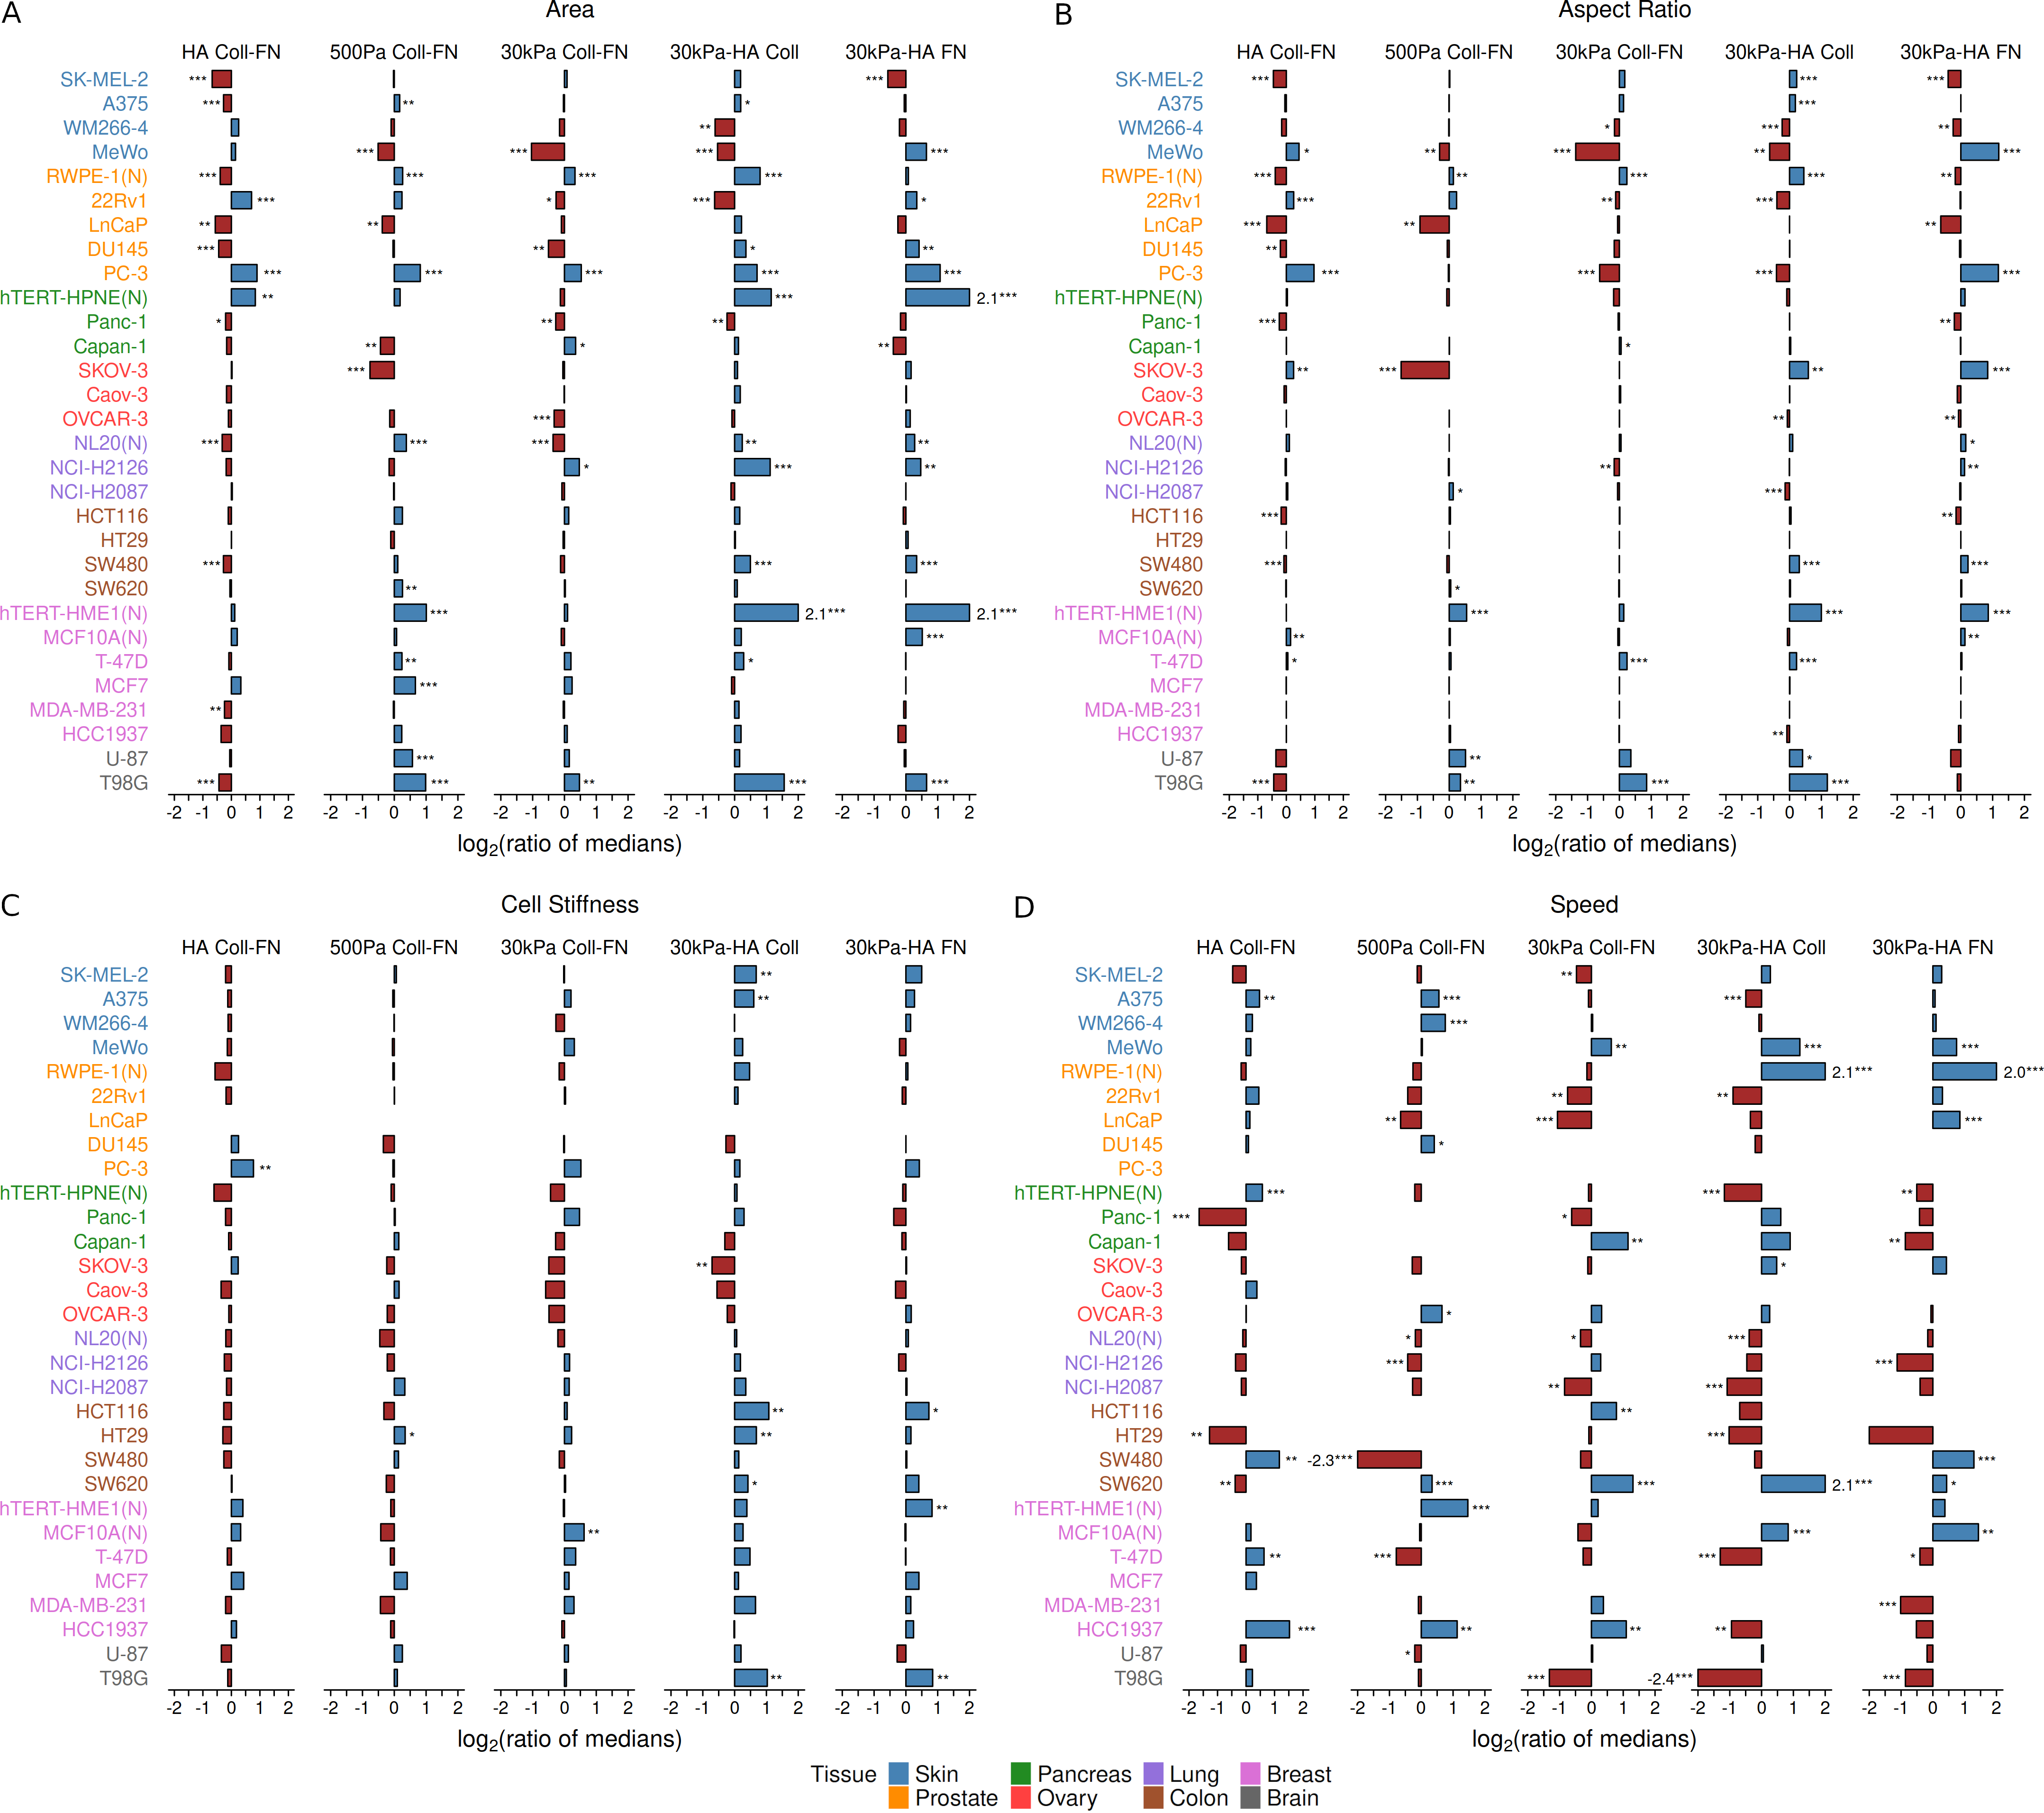
\includegraphics{../Figures/Supplementary_Figure2/supplementary_figure2.png}
    \caption{For each cell line, the ratio of the median values for (a) area and (b) cell stiffness as a measure of the phenotypic sensitivity to substrate change. 
    (HA Coll-FN: HA Coll/HA FN, 500Pa Coll-FN: 500Pa FN/500Pa Coll, 30kPa Coll-FN: 30kPa Coll/30kPa FN, 30kPa-HA Coll: 30kPa Coll/HA Coll, 30kPa-HA FN: 30kPa FN/HA FN, 
    Glass-30kPa Coll: Glass/30kPa Coll, Glass-30kPa FN: Glass/30kPa FN). (N) refers to non-malignant (normal) cell lines. 
    ***p-value < 0.01; **p-value < 0.05; *p-value < 0.1, adjusted for multiple testing using Benjamini-Hochberg procedure. 
    For each cell line, phenotypic sensitivity to substrate change is calculated only if there are at least 25 data points $(n \geq 25)$ for the physical feature of interest on both the substrates.
    See supplementary tables 1 and 2 for the exact value of $n$ for the cell lines.}
    \label{fig:fig2}
\end{figure}

\begin{figure}[H]
    \centering
    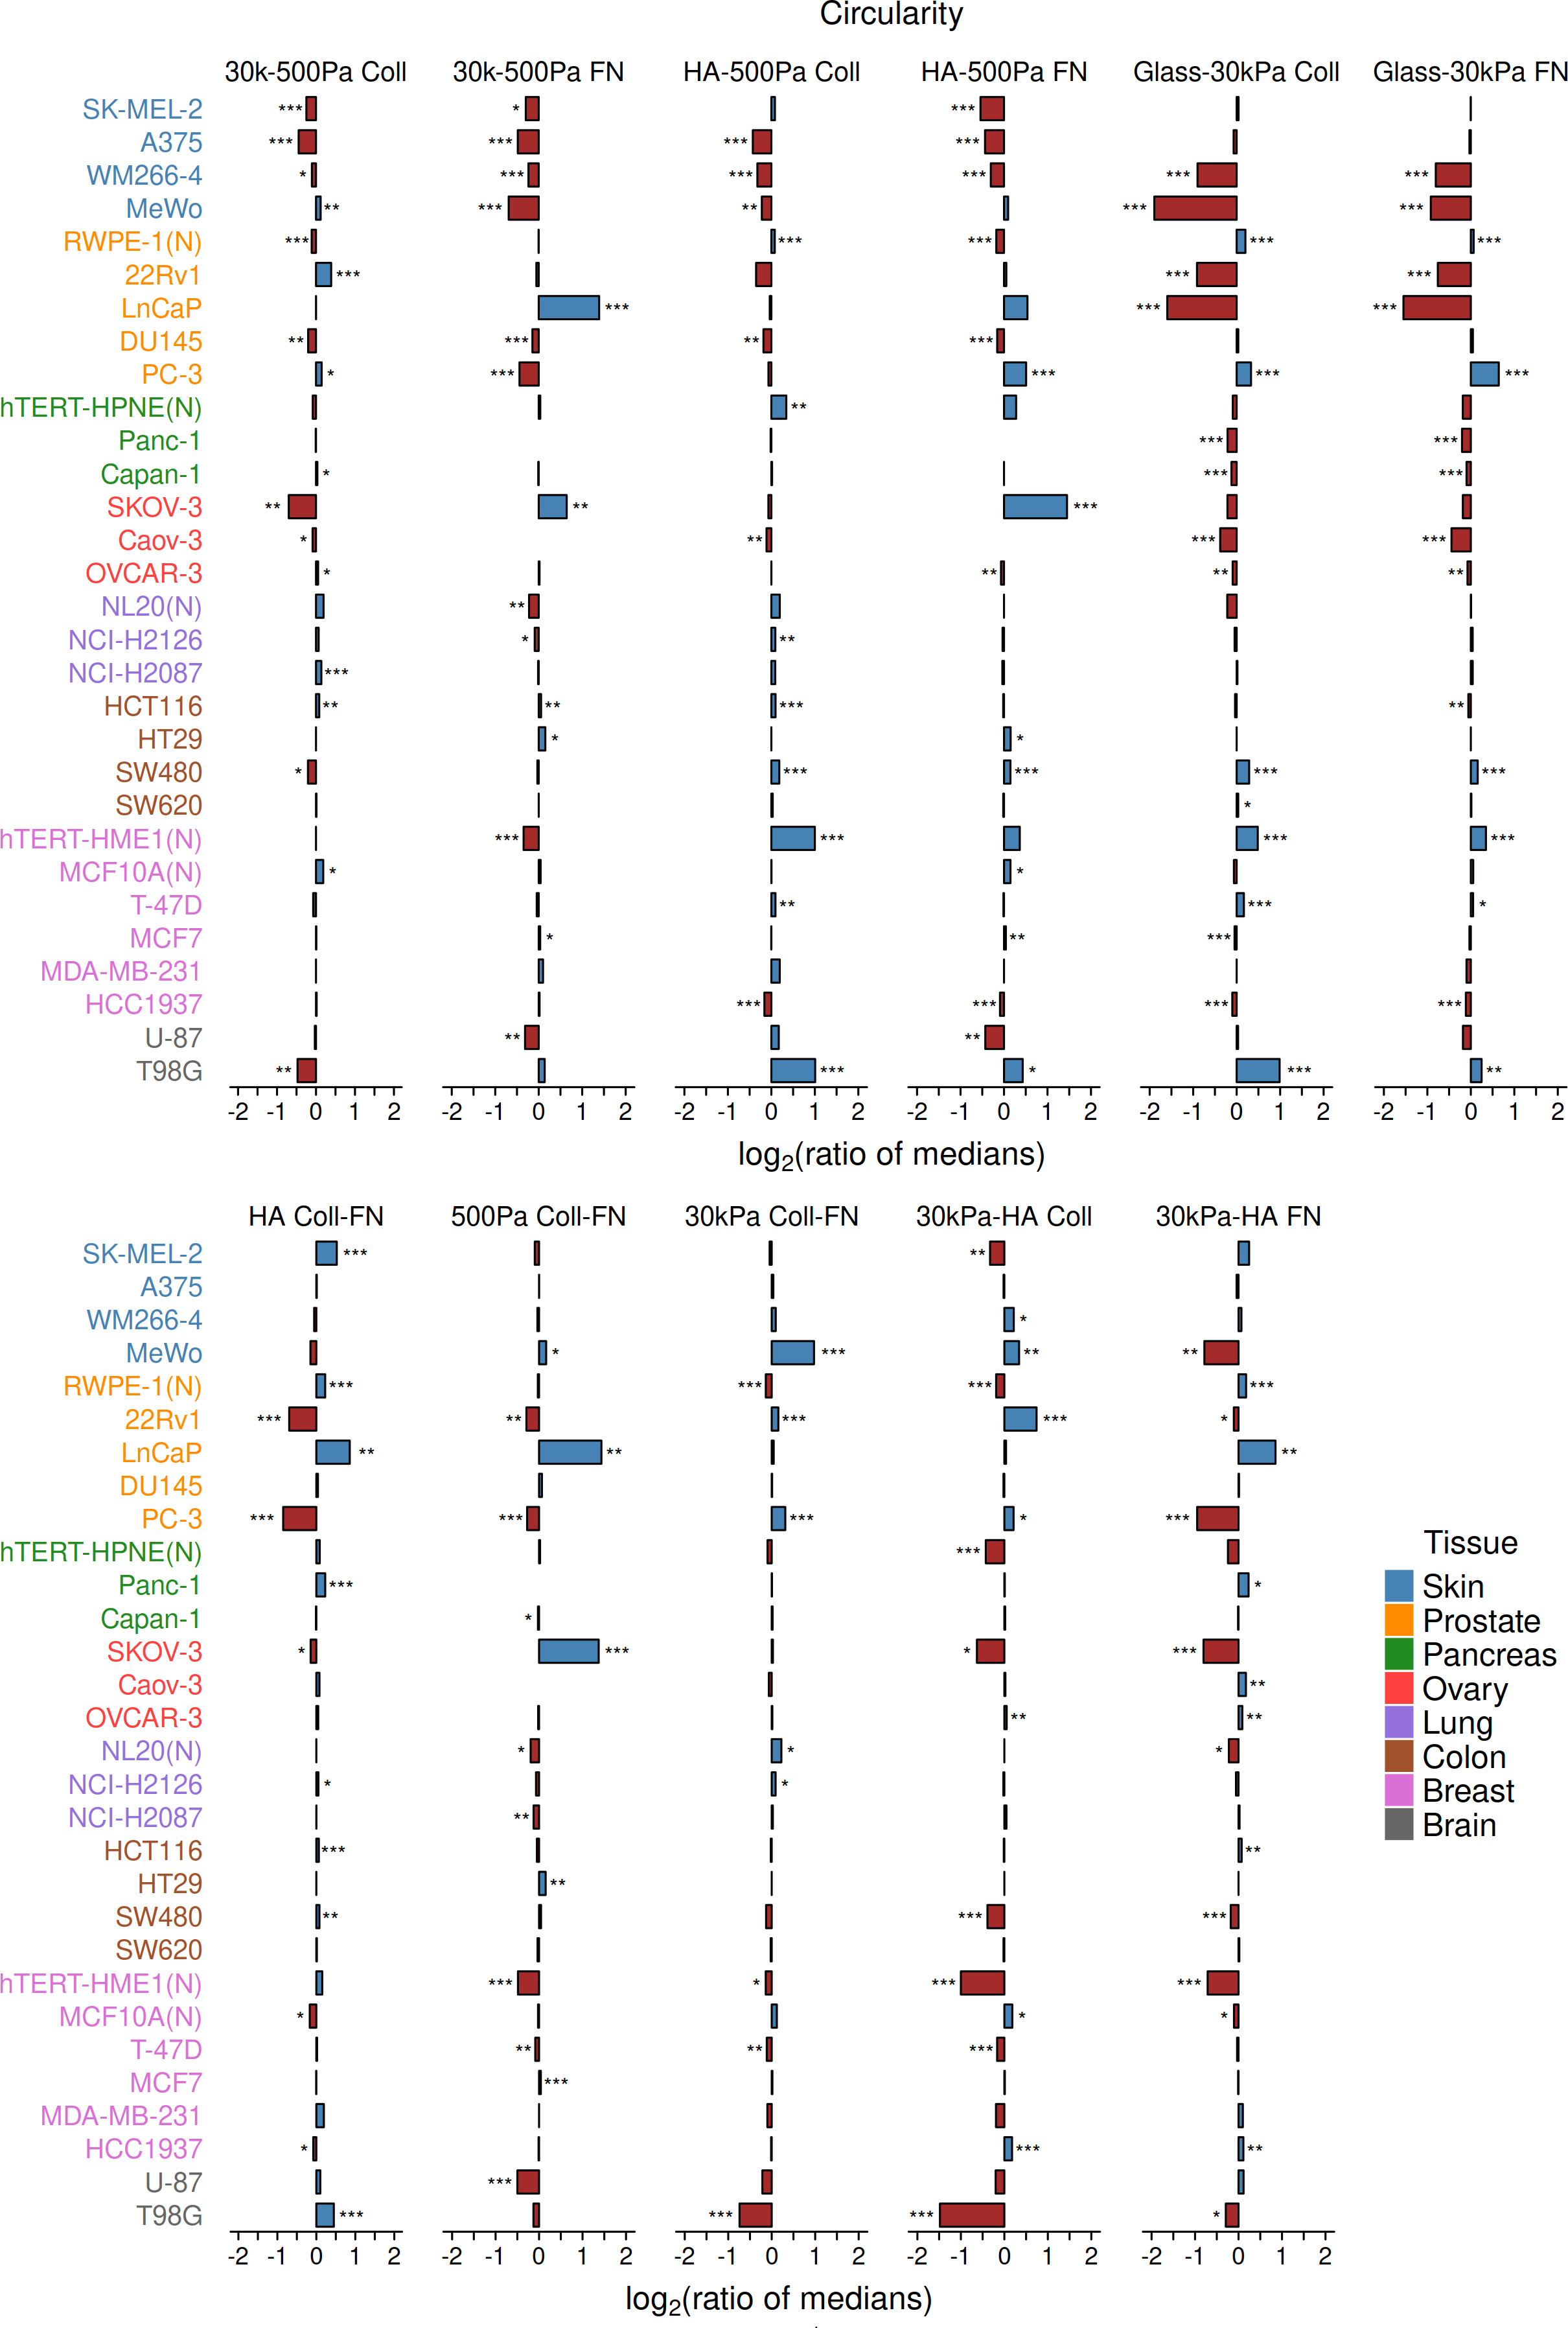
\includegraphics{../Figures/Supplementary_Figure3/supplementary_figure3.png}
    \caption{For each cell line, the ratio of the median values for cell speed as a measure of the phenotypic sensitivity to substrate change. 
    (HA Coll-FN: HA Coll/HA FN, 500Pa Coll-FN: 500Pa FN/500Pa Coll, 30kPa Coll-FN: 30kPa Coll/30kPa FN, 30kPa-HA Coll: 30kPa Coll/HA Coll, 30kPa-HA FN: 30kPa FN/HA FN,
    Glass-30kPa Coll: Glass/30kPa Coll, Glass-30kPa FN: Glass/30kPa FN). (N) refers to non-malignant (normal) cell lines. 
    ***p-value < 0.01; **p-value < 0.05; *p-value < 0.1, adjusted for multiple testing using Benjamini-Hochberg procedure. 
    For each cell line on a particular substrate, $n \geq 25$ cells. 
    See supplementary tables 3 for the exact value of $n$ for the cell lines.}
    \label{fig:fig3}
\end{figure}

\begin{figure}[H]
    \vspace*{-0.65cm}
    \centering
    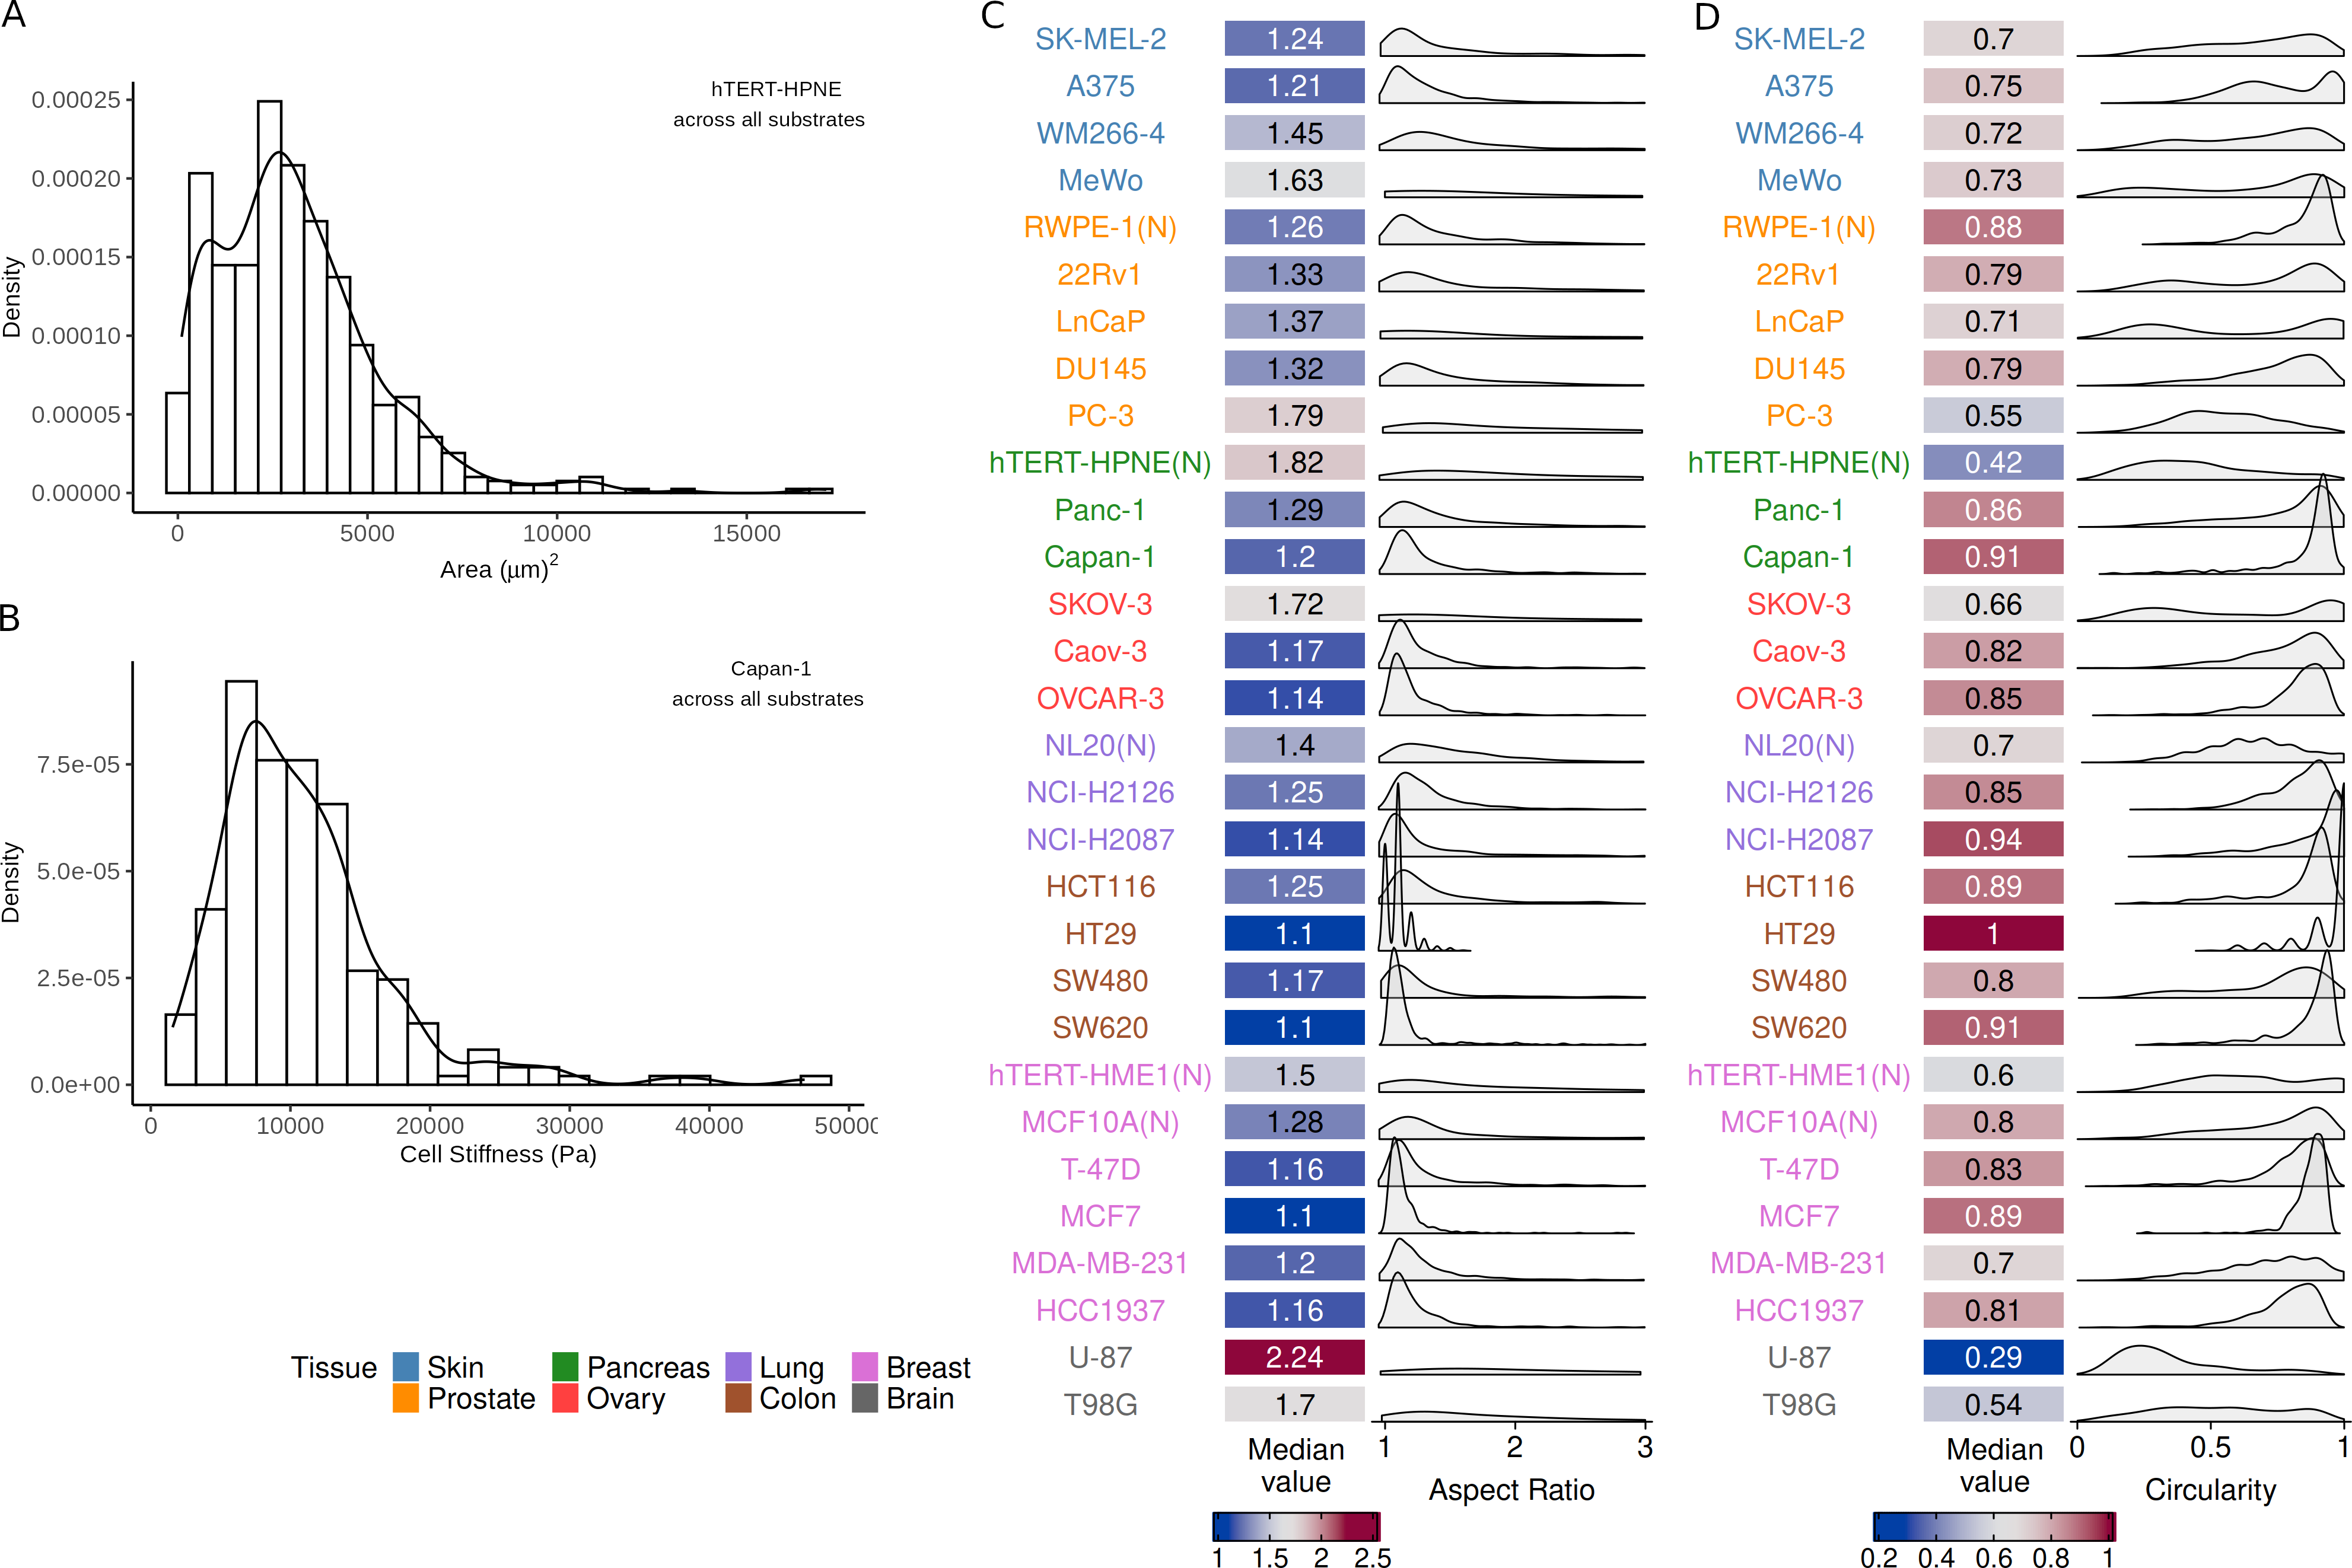
\includegraphics{../Figures/Supplementary_Figure4/supplementary_figure4.png}
    \caption{For each cell line, the ratio of the median values for aspect ratio as a measure of the phenotypic sensitivity to substrate change. 
    (30k-500Pa Coll: 30kPa Coll/500Pa Coll, 30k-500Pa FN: 30kPa FN/500Pa FN, HA-500Pa Coll: HA Coll/500Pa Coll, HA-500Pa  FN: HA FN/500Pa FN, Glass-30kPa Coll: Glass/30kPa Coll, Glass-30kPa FN: Glass/30kPa FN, 
    HA Coll-FN: HA Coll/HA FN, 500Pa Coll-FN: 500Pa FN/500Pa Coll, 30kPa Coll-FN: 30kPa Coll/30kPa FN, 30kPa-HA Coll: 30kPa Coll/HA Coll, 30kPa-HA FN: 30kPa FN/HA FN). (N) refers to non-malignant (normal) cell lines.
    ***p-value < 0.01; **p-value < 0.05; *p-value < 0.1, adjusted for multiple testing using Benjamini-Hochberg procedure. 
    For each cell line on a particular substrate, $n \geq 25$ cells.
    See supplementary tables 1 for the exact value of $n$ for the cell lines.}
    \label{fig:fig4}
\end{figure}

\begin{figure}[H]
    \vspace*{-0.65cm}
    \centering
    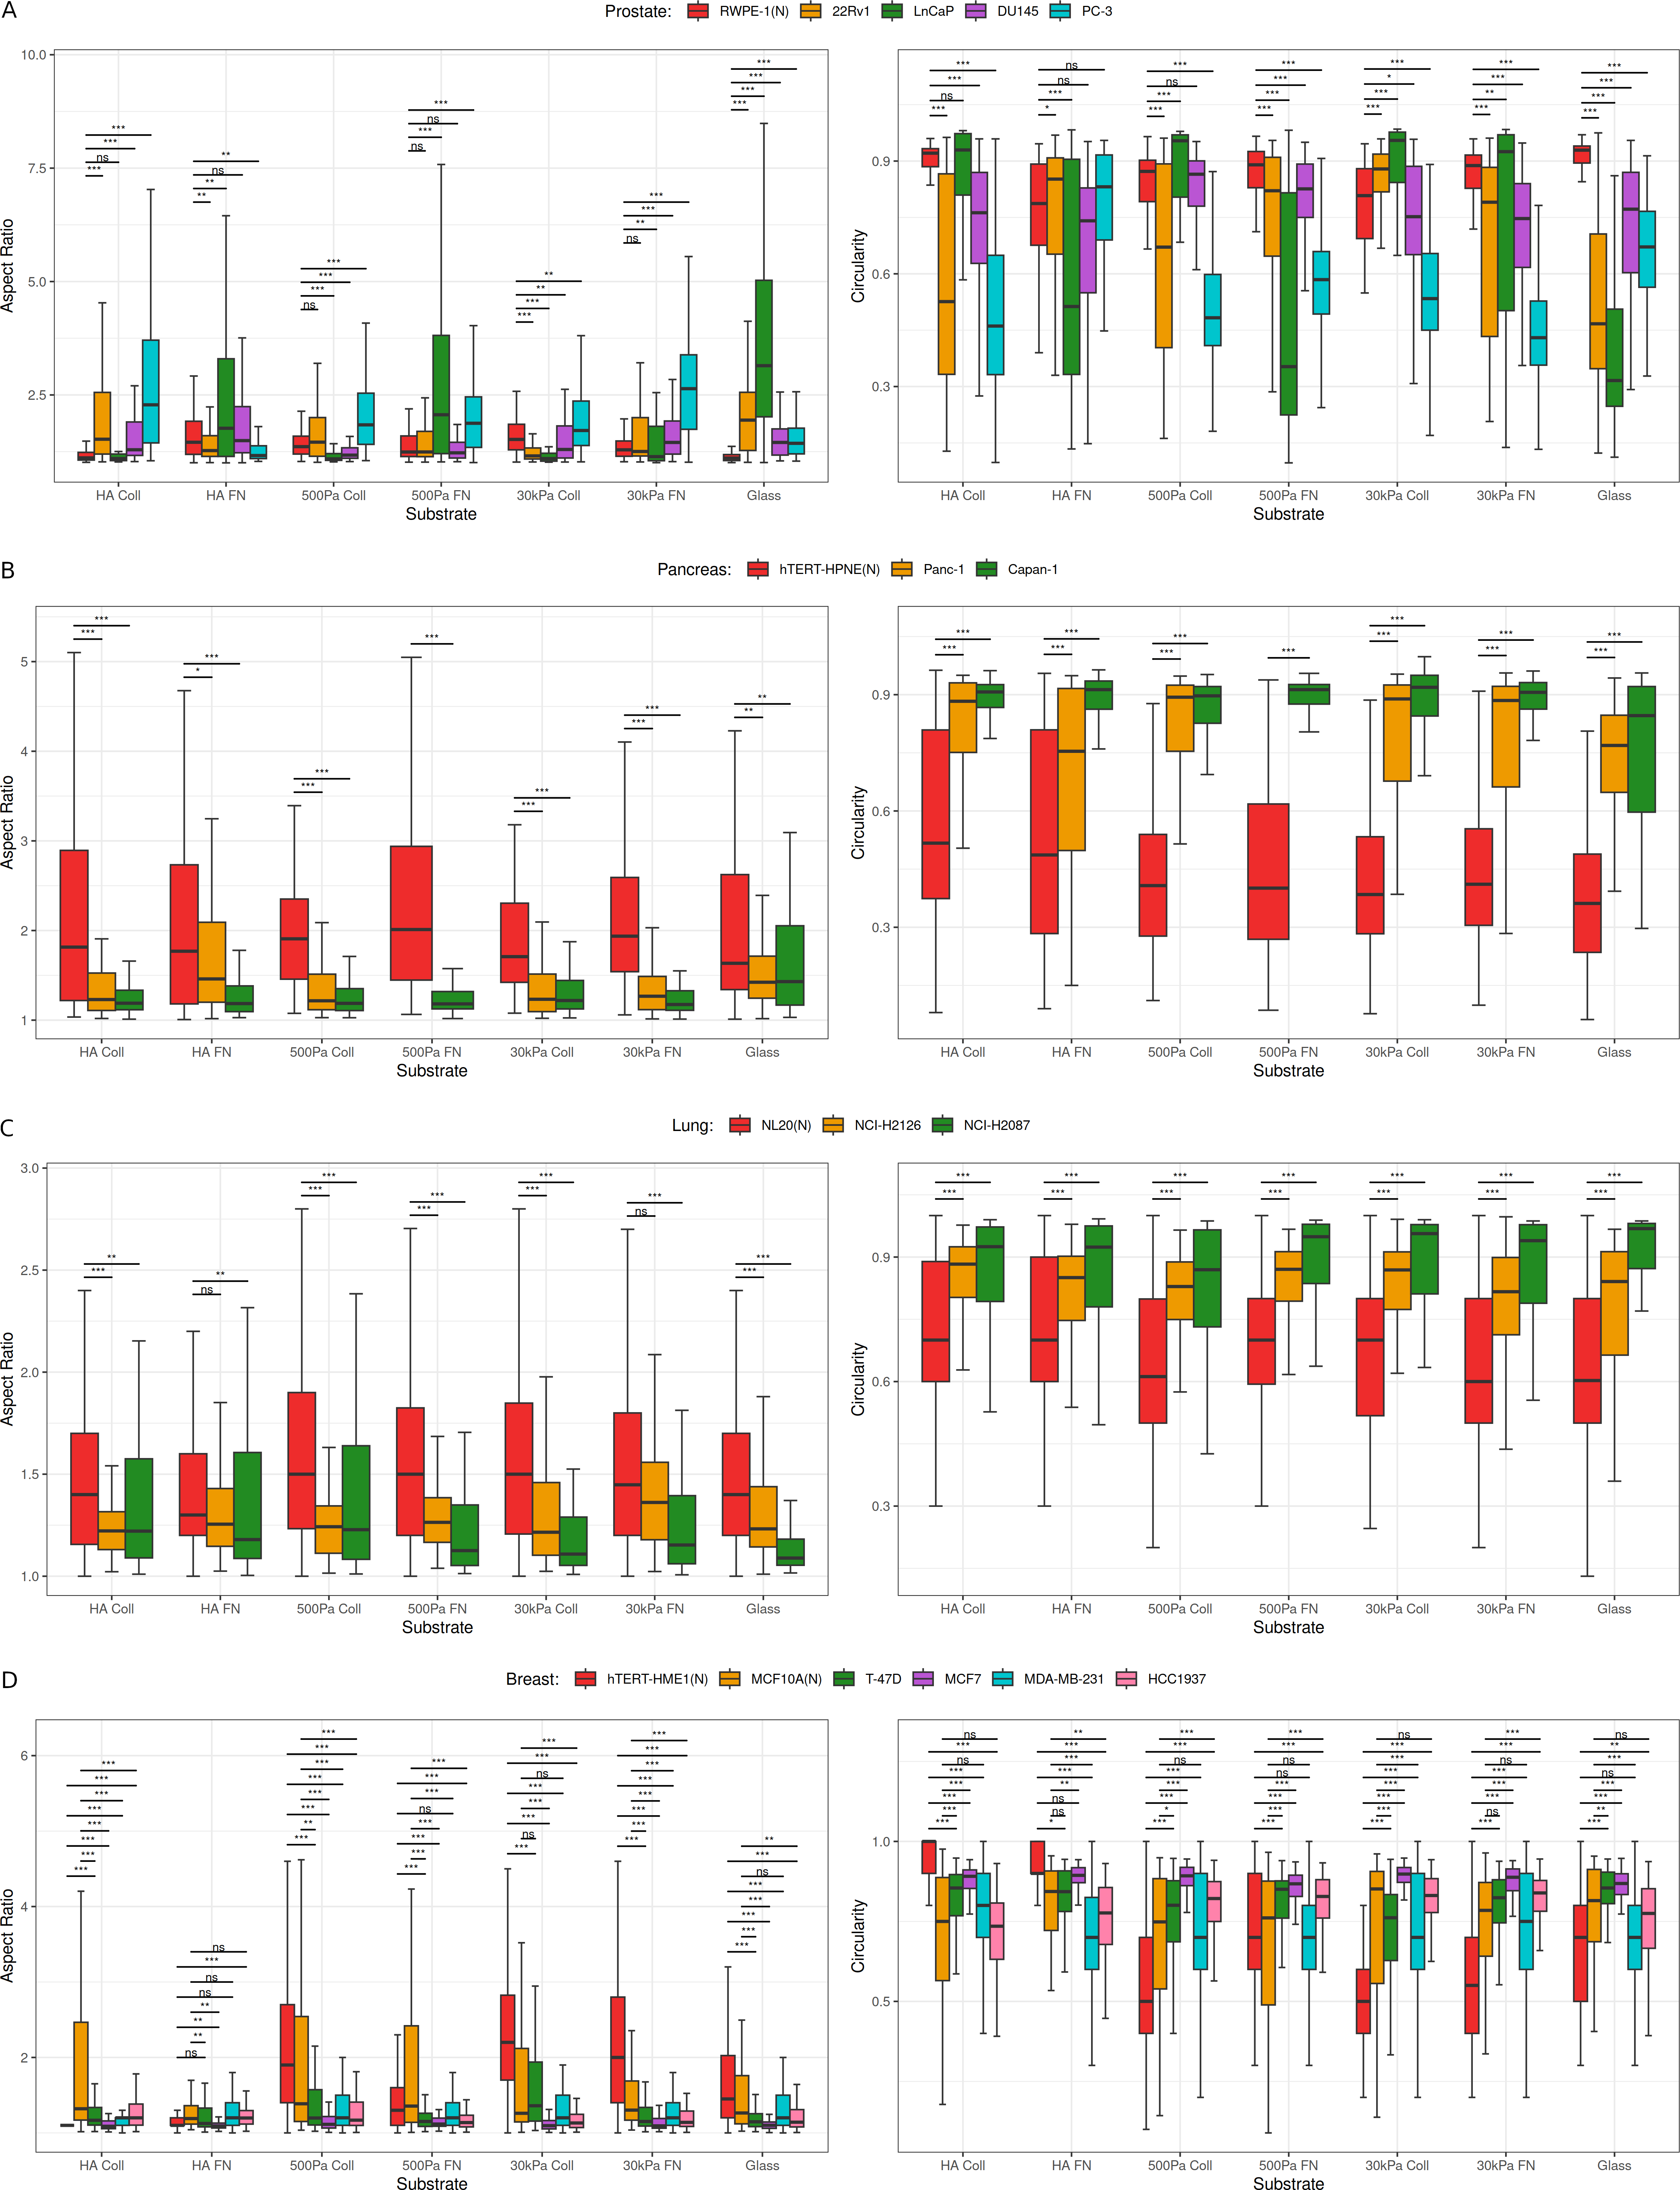
\includegraphics{../Figures/Supplementary_Figure5/supplementary_figure5.png}
    \caption{For each cell line, the ratio of the median values for circularity as a measure of the phenotypic sensitivity to substrate change. 
    (30k-500Pa Coll: 30kPa Coll/500Pa Coll, 30k-500Pa FN: 30kPa FN/500Pa FN, HA-500Pa Coll: HA Coll/500Pa Coll, HA-500Pa  FN: HA FN/500Pa FN, Glass-30kPa Coll: Glass/30kPa Coll, Glass-30kPa FN: Glass/30kPa FN, 
    HA Coll-FN: HA Coll/HA FN, 500Pa Coll-FN: 500Pa FN/500Pa Coll, 30kPa Coll-FN: 30kPa Coll/30kPa FN, 30kPa-HA Coll: 30kPa Coll/HA Coll, 30kPa-HA FN: 30kPa FN/HA FN). (N) refers to non-malignant (normal) cell lines.
    ***p-value < 0.01; **p-value < 0.05; *p-value < 0.1, adjusted for multiple testing using Benjamini-Hochberg procedure. 
    For each cell line on a particular substrate, $n \geq 25$ cells.
    See supplementary tables 1 for the exact value of $n$ for the cell lines.}
    \label{fig:fig5}
\end{figure}

\begin{figure}[H]
    \centering
    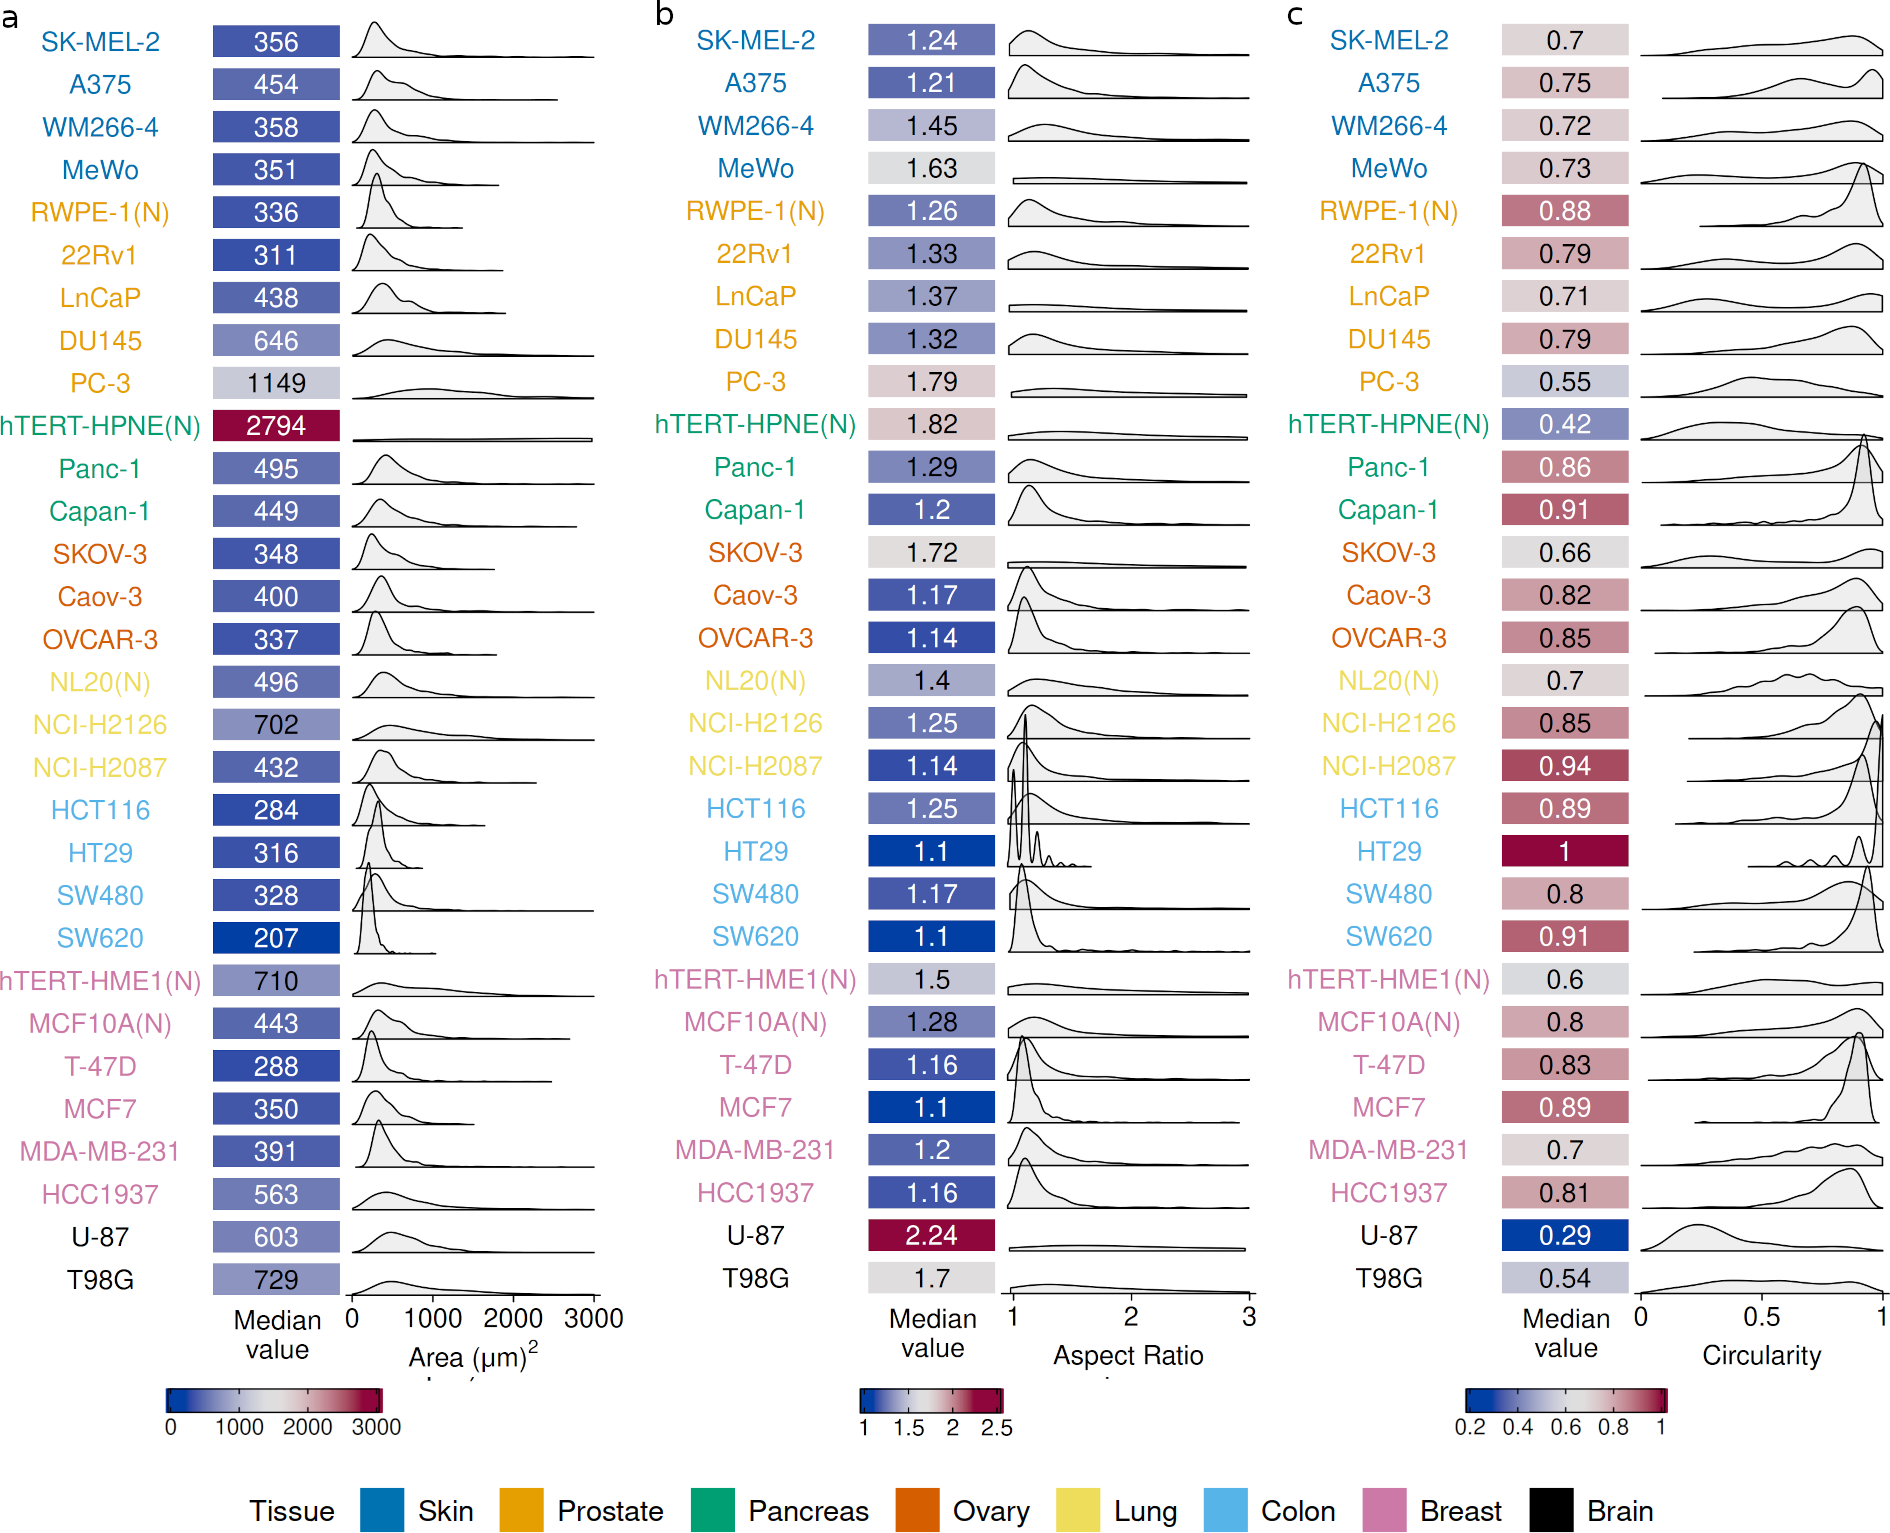
\includegraphics{../Figures/Supplementary_Figure6/supplementary_figure6.png}
    \caption{Median values of cell (a) area, (b) aspect ratio, and (c) circularity across all the 7 different substrates, along with the kernel density estimates (KDE) for summarizing the distribution of feature values for each cell line. (N) refers to non-malignant (normal) cell lines.
    See supplementary figure 7c for the KDE of outlier-like distributions of hTERT-HPNE cellular area across all substrates.}
    \label{fig:fig6}
\end{figure}

\begin{figure}[H]
    \hspace*{-0.8cm}
    \centering
    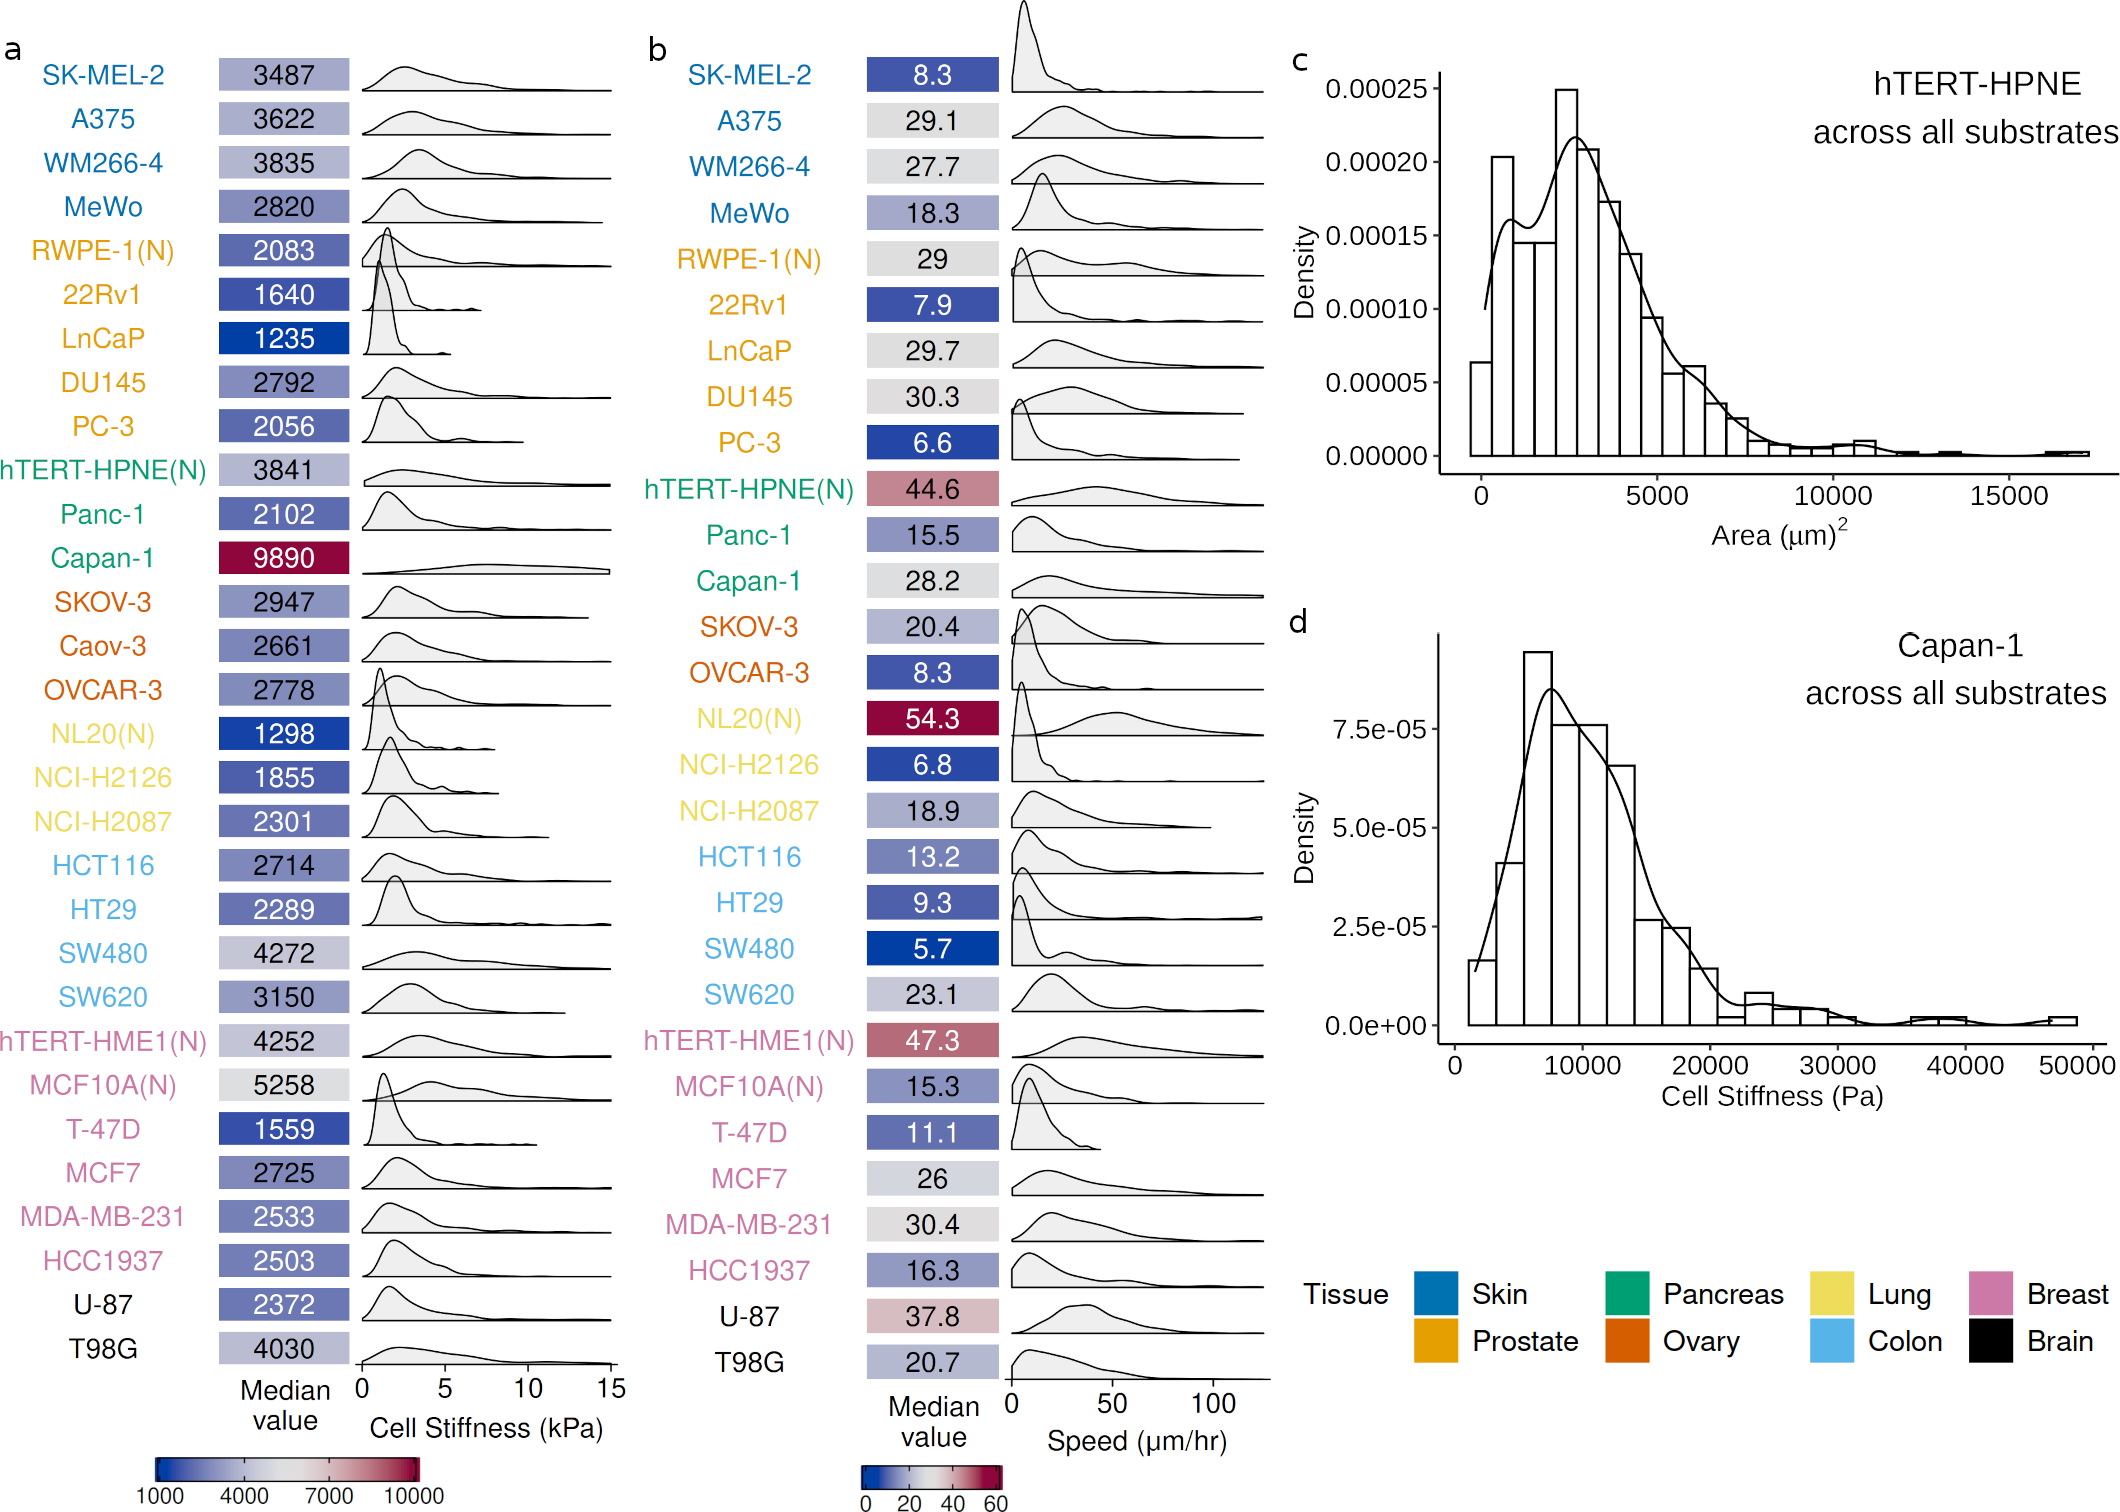
\includegraphics{../Figures/Supplementary_Figure7/supplementary_figure7.png}
    \caption{Median values of (a) cell stiffness and (b) cell speed across all the 7 different substrates, along with the kernel density estimates (KDE) for summarizing the distribution of feature values for each cell line. (N) refers to non-malignant (normal) cell lines.
    KDEs for outlier-like distributions of (c) hTERT-HPNE cellular area across all substrates, and (d) Capan-1 cell stiffness across all substrates.}
    \label{fig:fig7}
\end{figure}

\begin{figure}[H]
    \hspace*{-0.8cm}
    \centering
    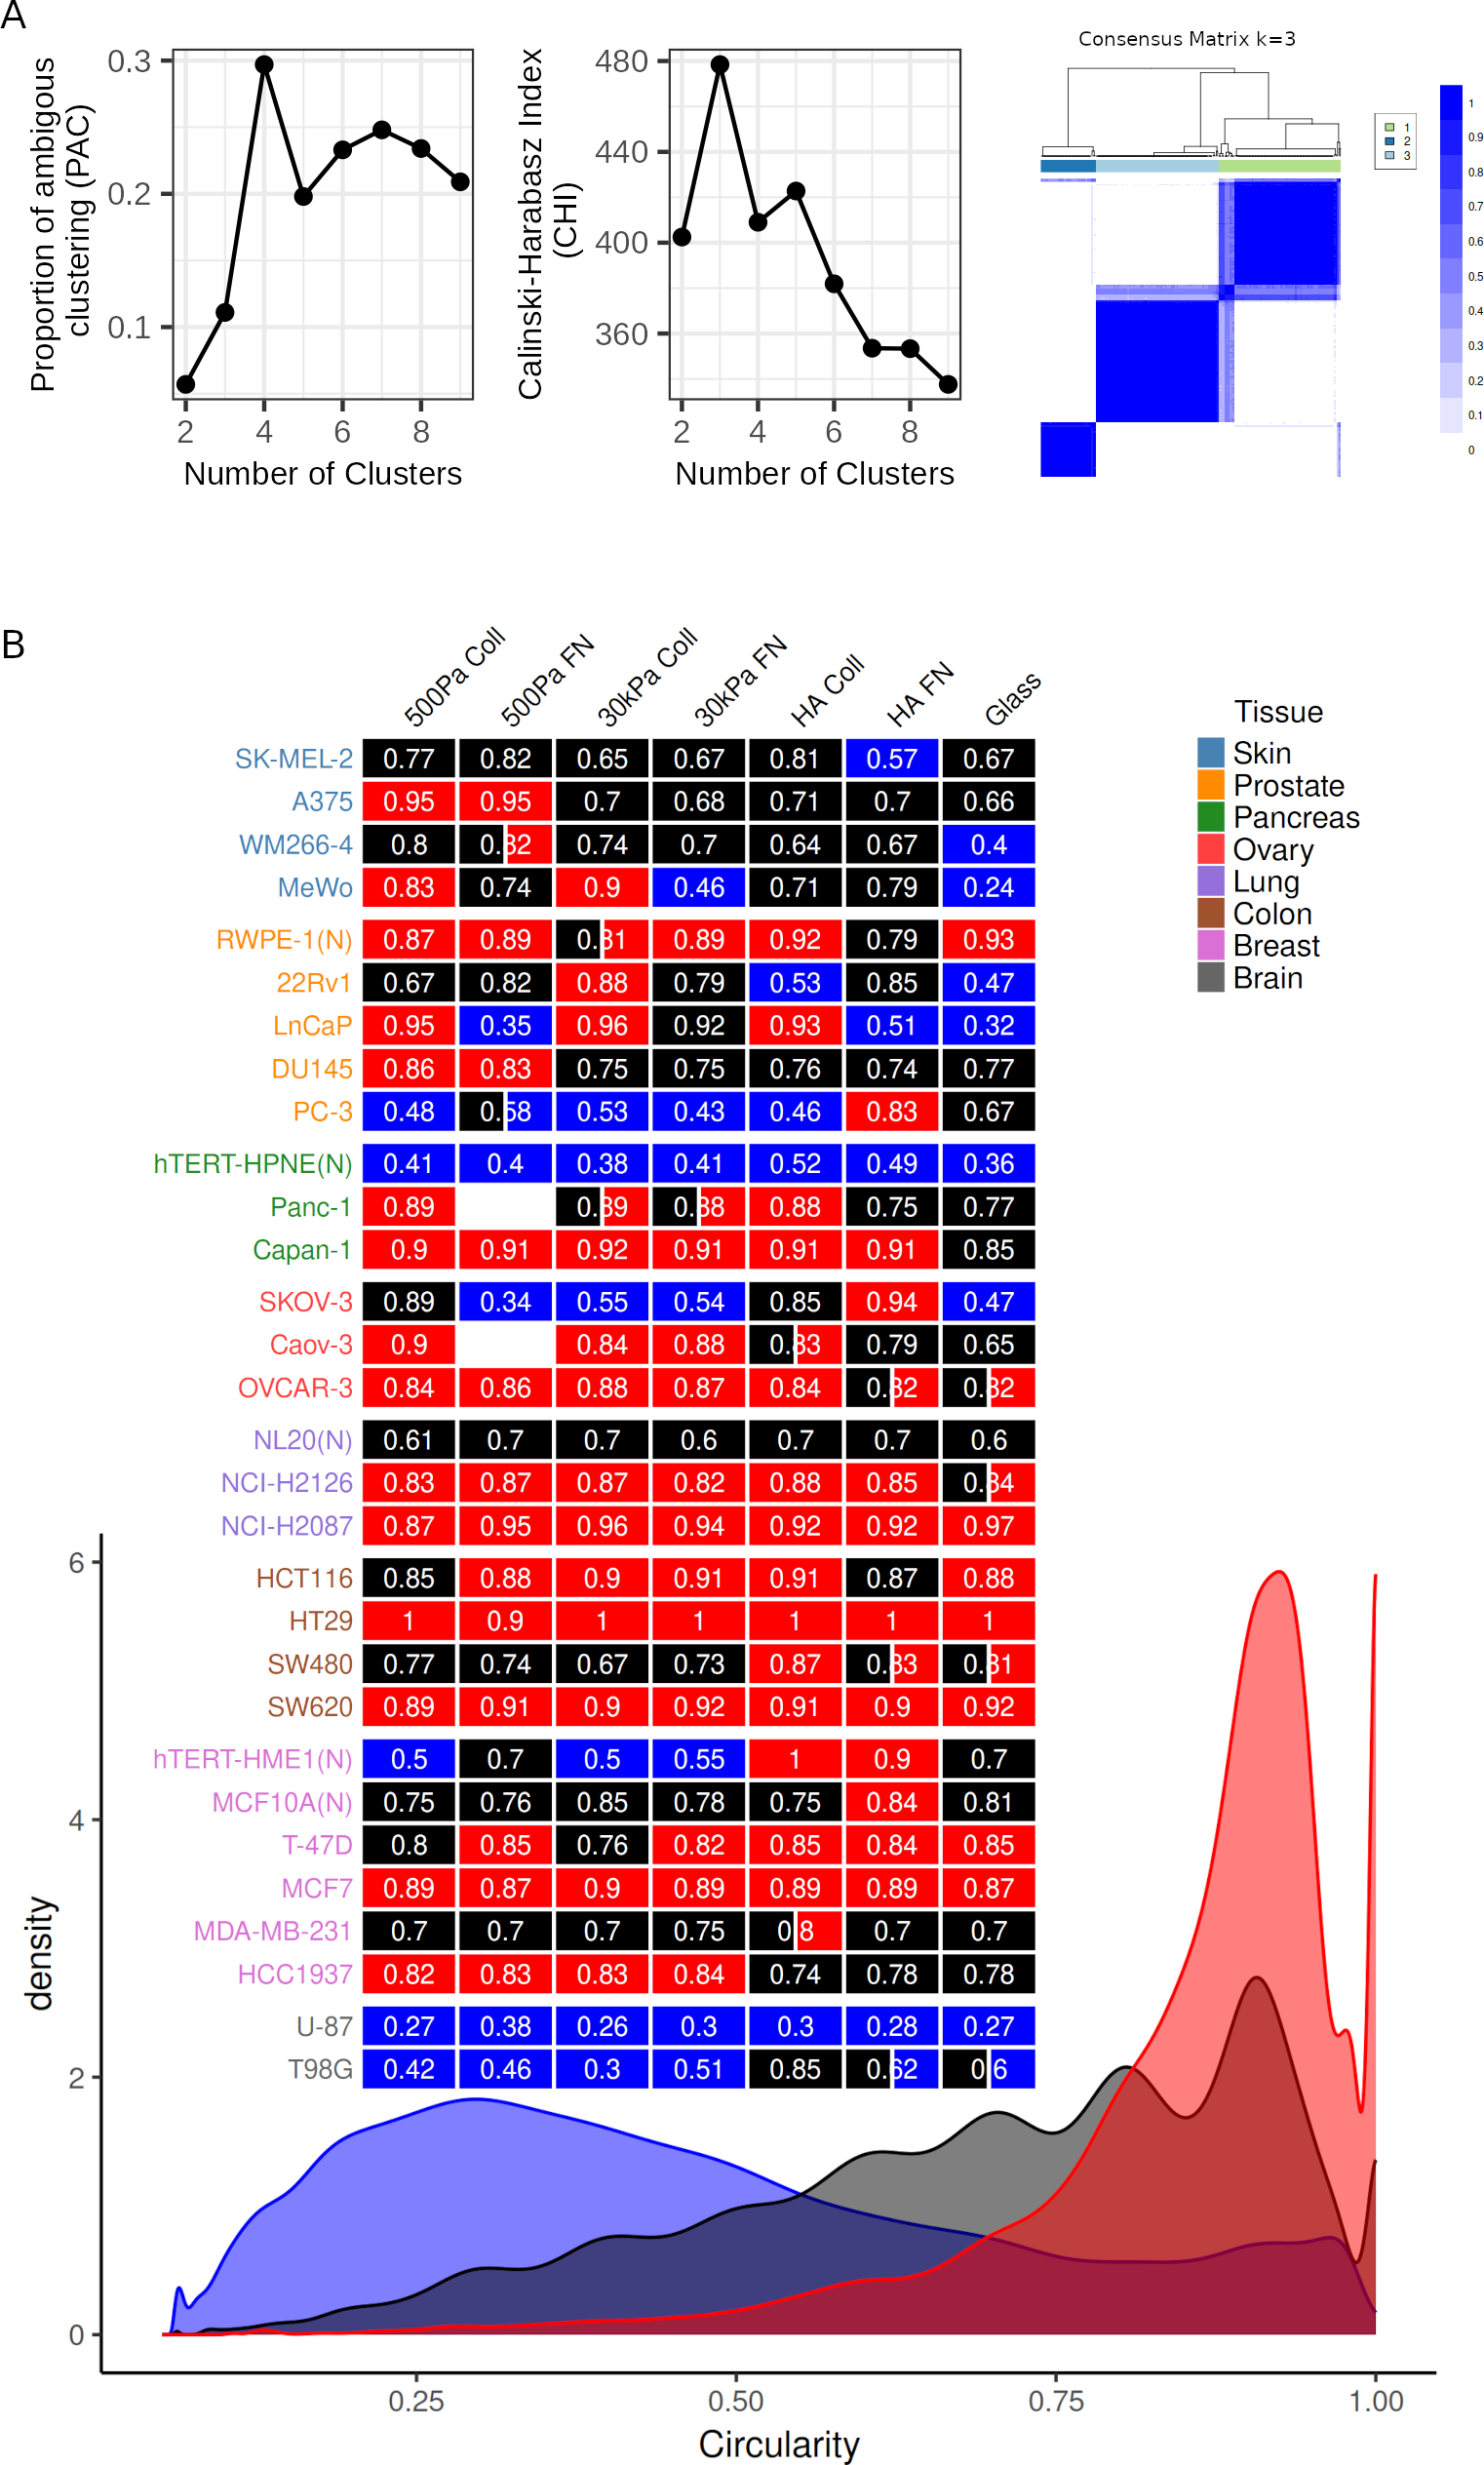
\includegraphics{../Figures/Supplementary_Figure8/supplementary_figure8.png}
    \caption{Comparing tissue-specific normal and cancer cell behavior in terms of cell (a) area, (b) aspect ratio, (c) stiffness, and (d) speed for pancreatic cell lines 
    soft (500 Pa) and stiff (30 kPa) PAAm Coll and FN substrates, soft (500 Pa) HA substrates coated with Coll and FN, and glass. (N) refers to non-malignant (normal) cell lines.
    ***p-value < 0.01; **p-value < 0.05; *p-value < 0.1, adjusted for multiple testing using Benjamini-Hochberg procedure. 
    The number of measurements for the physical feature of interest is at least 25 $(n \geq 25)$ for each cell line on a particular substrate. 
    See supplementary tables 1-3 for the exact value of $n$ for the cell lines.}
    \label{fig:fig8}
\end{figure}

\begin{figure}[H]
    \hspace*{-0.8cm}
    \centering
    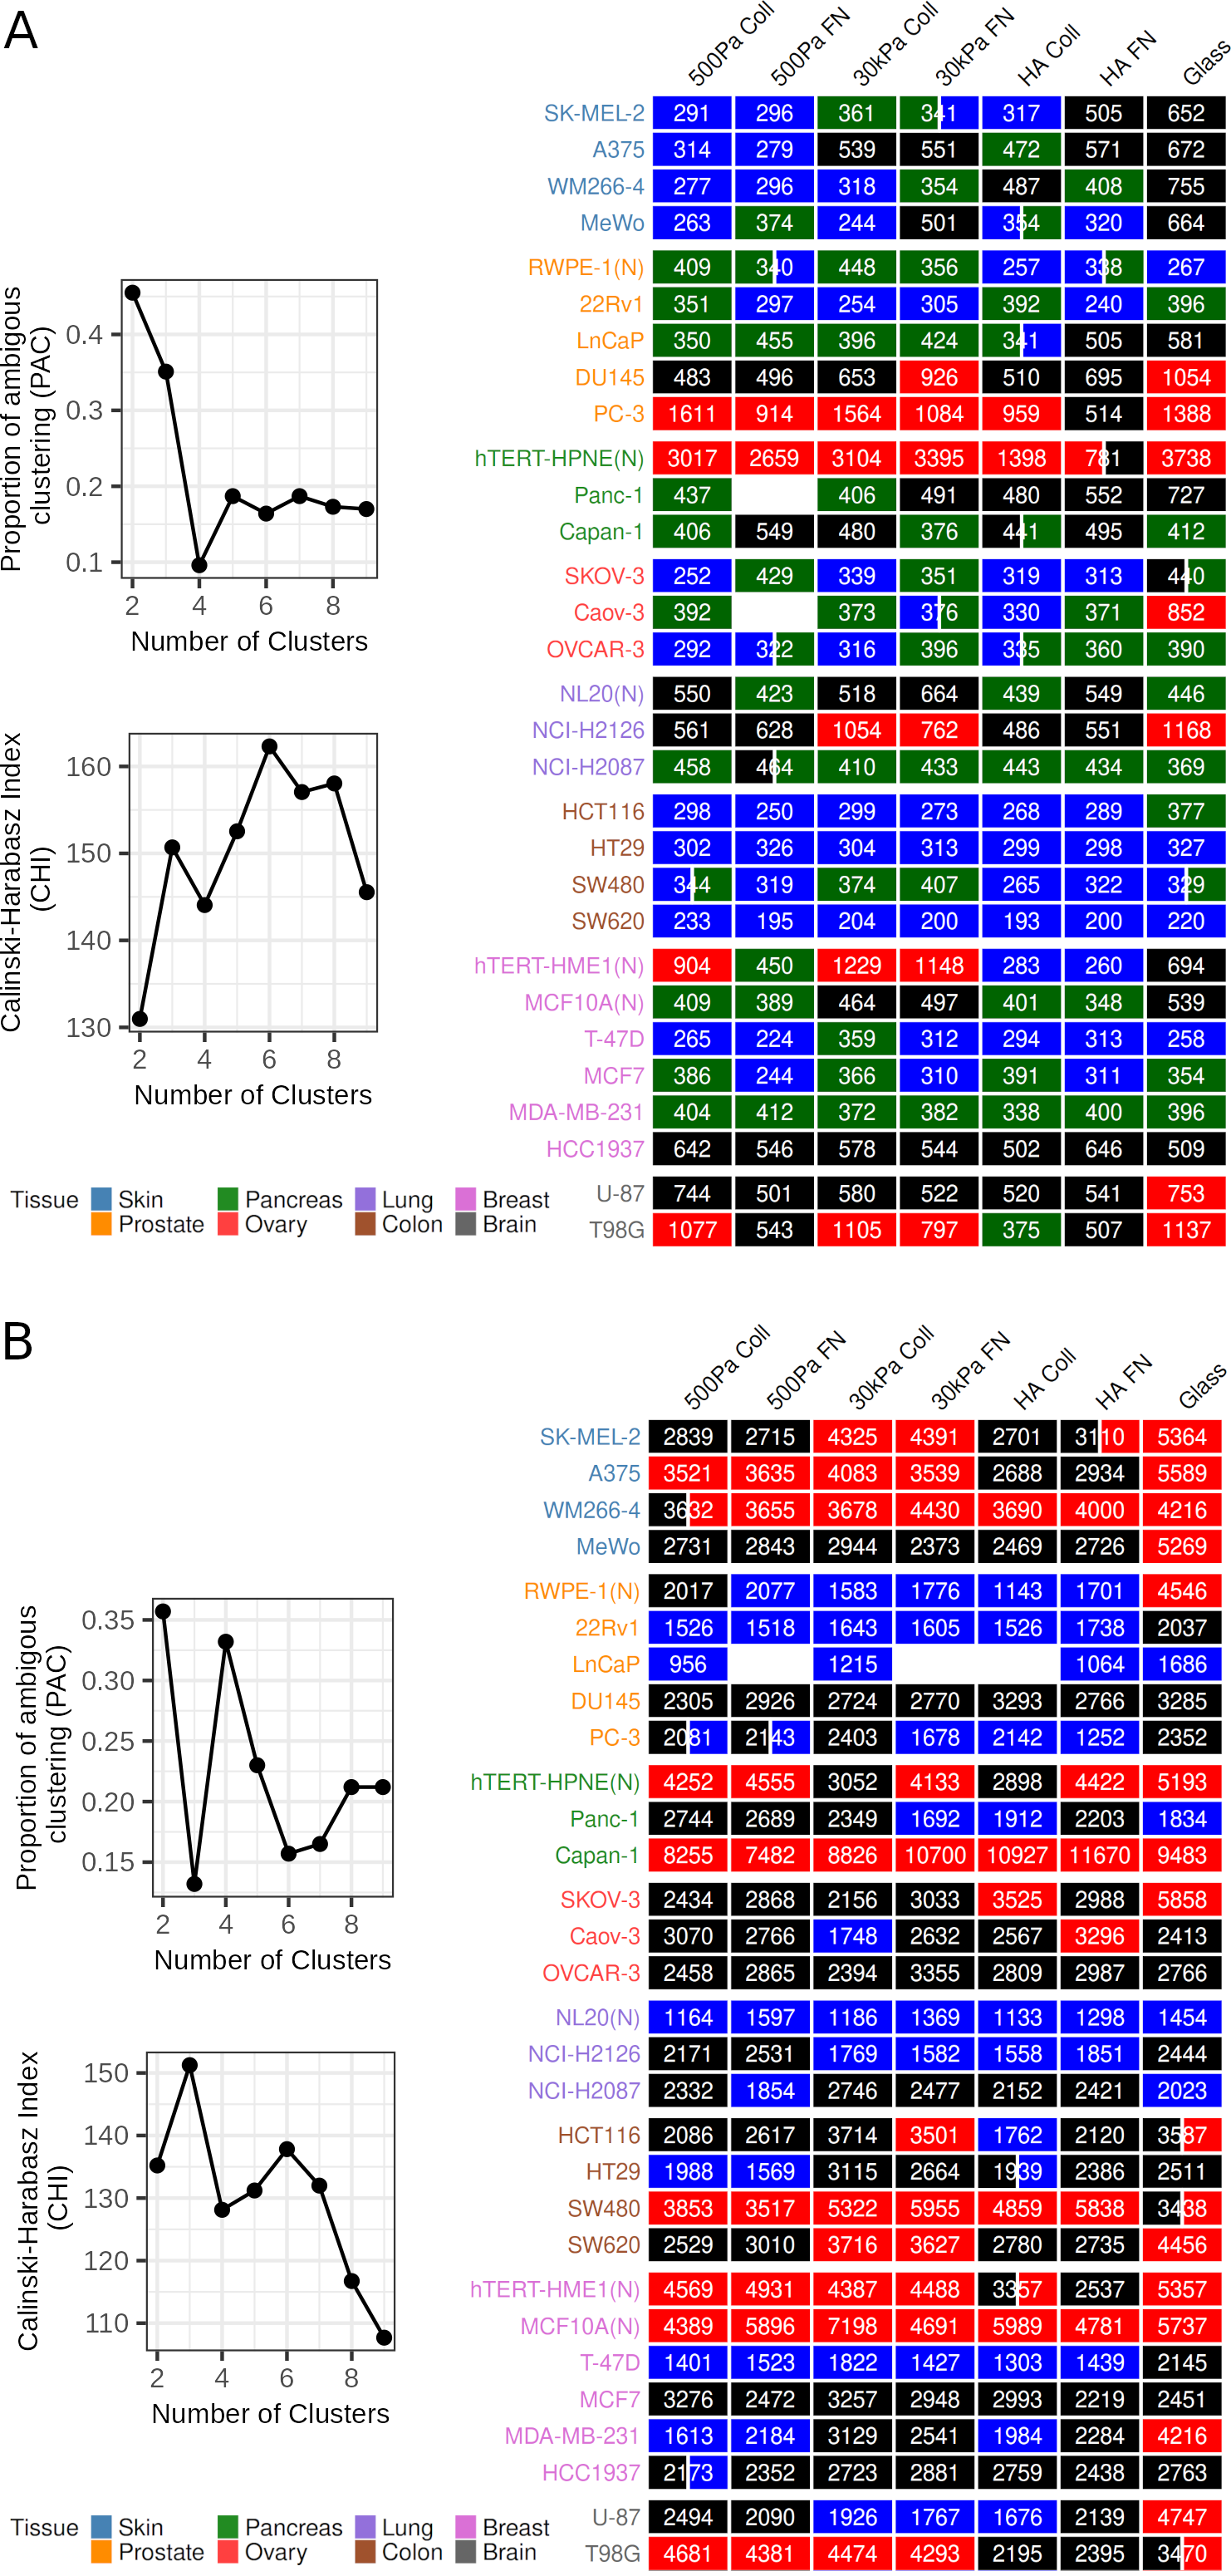
\includegraphics{../Figures/Supplementary_Figure9/supplementary_figure9.png}
    \caption{Comparing tissue-specific normal and cancer cell behavior in terms of aspect ratio, and cicularity for (a) breast, (b) lung, and (c) prostate cell lines 
    soft (500 Pa) and stiff (30 kPa) PAAm Coll and FN substrates, soft (500 Pa) HA substrates coated with Coll and FN, and glass. (N) refers to non-malignant (normal) cell lines.
    ***p-value < 0.01; **p-value < 0.05; *p-value < 0.1, adjusted for multiple testing using Benjamini-Hochberg procedure. 
    For each cell line on a particular substrate, $n \geq 25$ cells.
    See supplementary tables 1 for the exact value of $n$ for the cell lines.}
    \label{fig:fig9}
\end{figure}

\begin{figure}[H]
    \hspace*{-0.8cm}
    \vspace*{2cm}
    \centering
    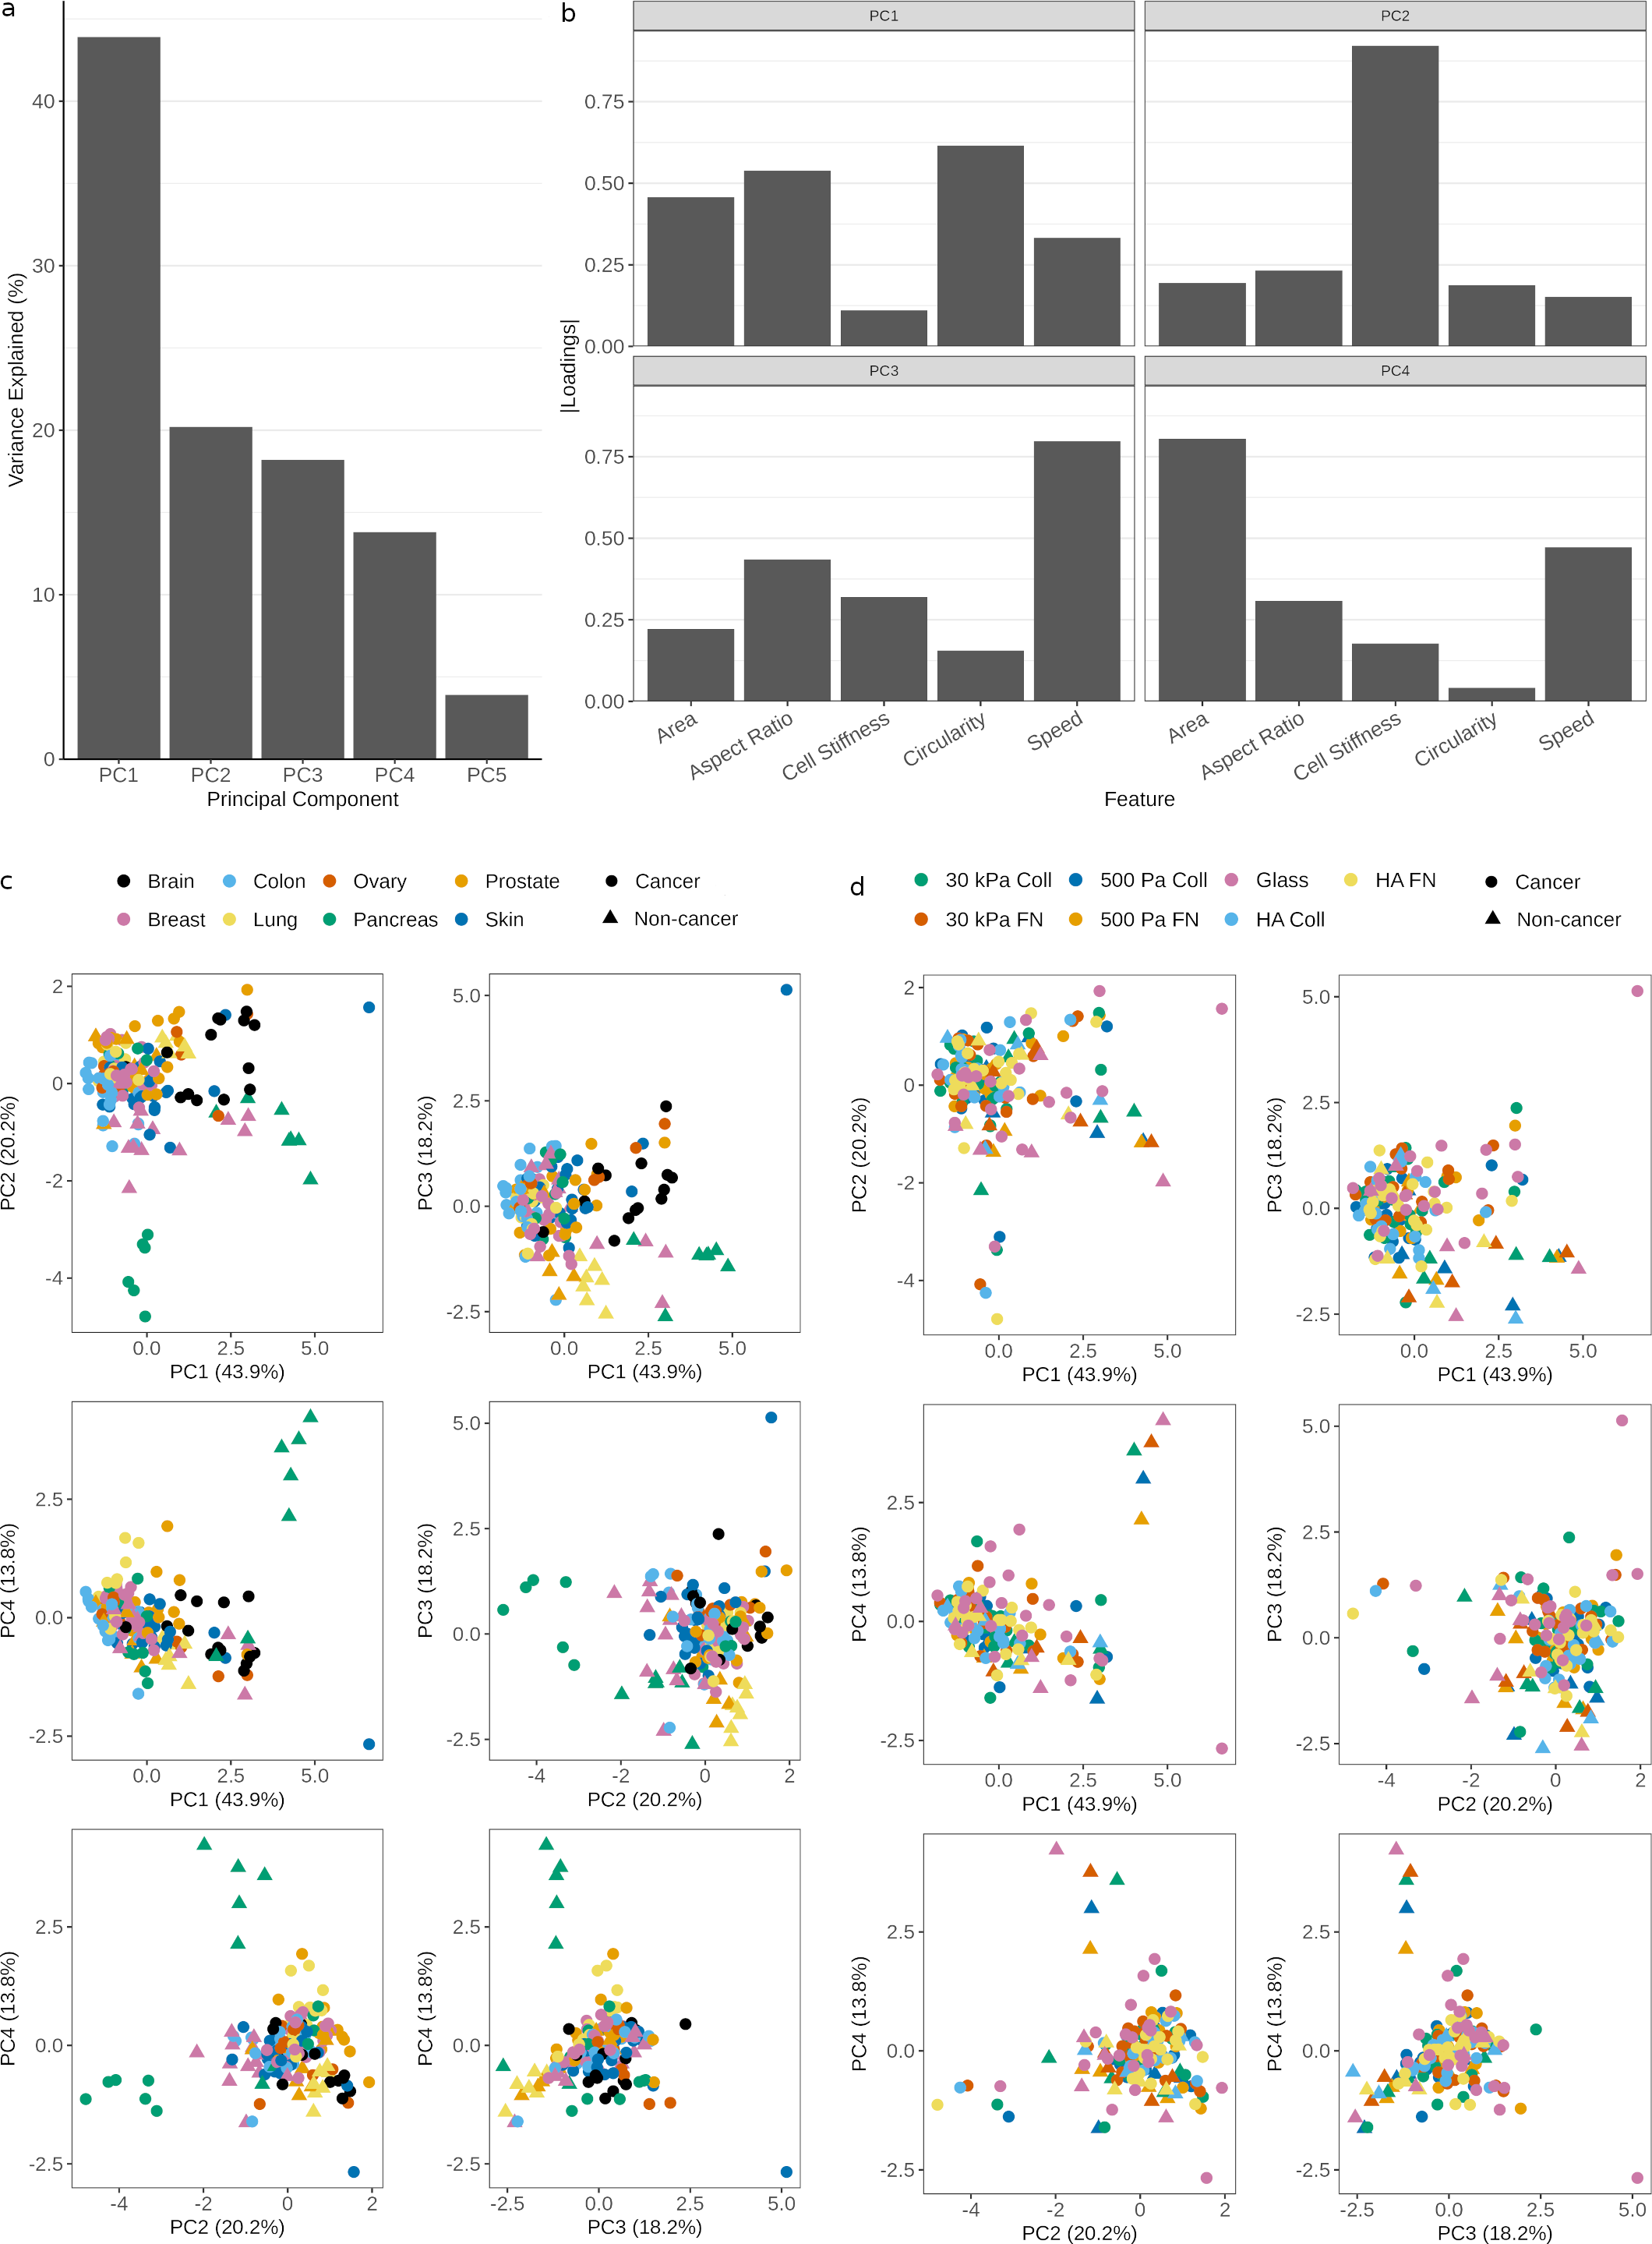
\includegraphics{../Figures/Supplementary_Figure10/supplementary_figure10.png}
    \caption{}
    \label{fig:fig10}
\end{figure}
\begin{adjustwidth}{1cm}{1cm}
    Supplementary Figure 10: Principal component analysis (PCA) performed using the median values of cell area, aspect ratio, circularity, stiffness, and speedfrom all the cell line-substrate pairs.
    Note that in this analysis only those cell line-substrate pairs are considered which have at least 25 data points for each of the physical feature.
    (a) Variance explained by each of the PCs, and (b) the loadings of the physical features on the first four PCs.
    Pairwise scatter plots for the first four PCs, with the points colored by the (c) tissue type and (d) substrate type. 
\end{adjustwidth}

\begin{figure}[H]
    \centering
    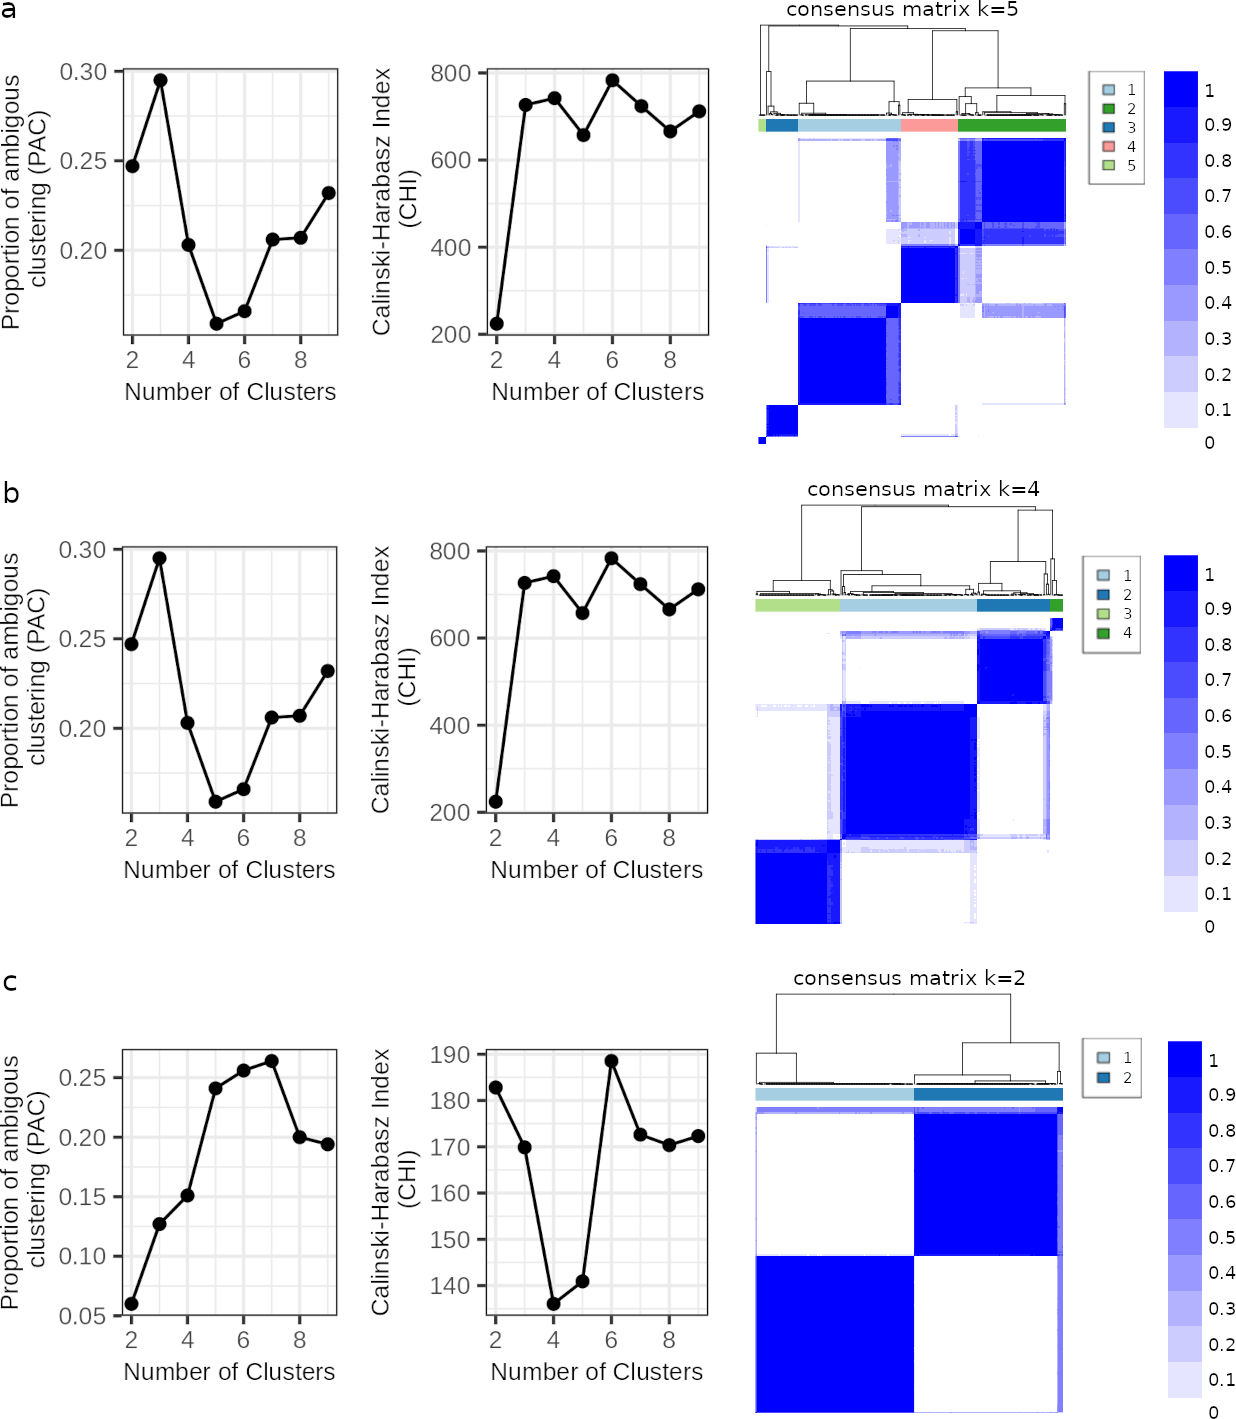
\includegraphics{../Figures/Supplementary_Figure11/supplementary_figure11.png}
    \caption{Clustering statistics (PAC and CHI) used for identifying the optimal number of clusters (mechanotypes) based on Wasserstein-1 distance and the corresponding consensus matrix for optimal cluster count $k$
    of cell (a) area, (b) stiffness, and (c) speed.}
    \label{fig:fig11}
\end{figure}

\begin{figure}[H]
    \centering
    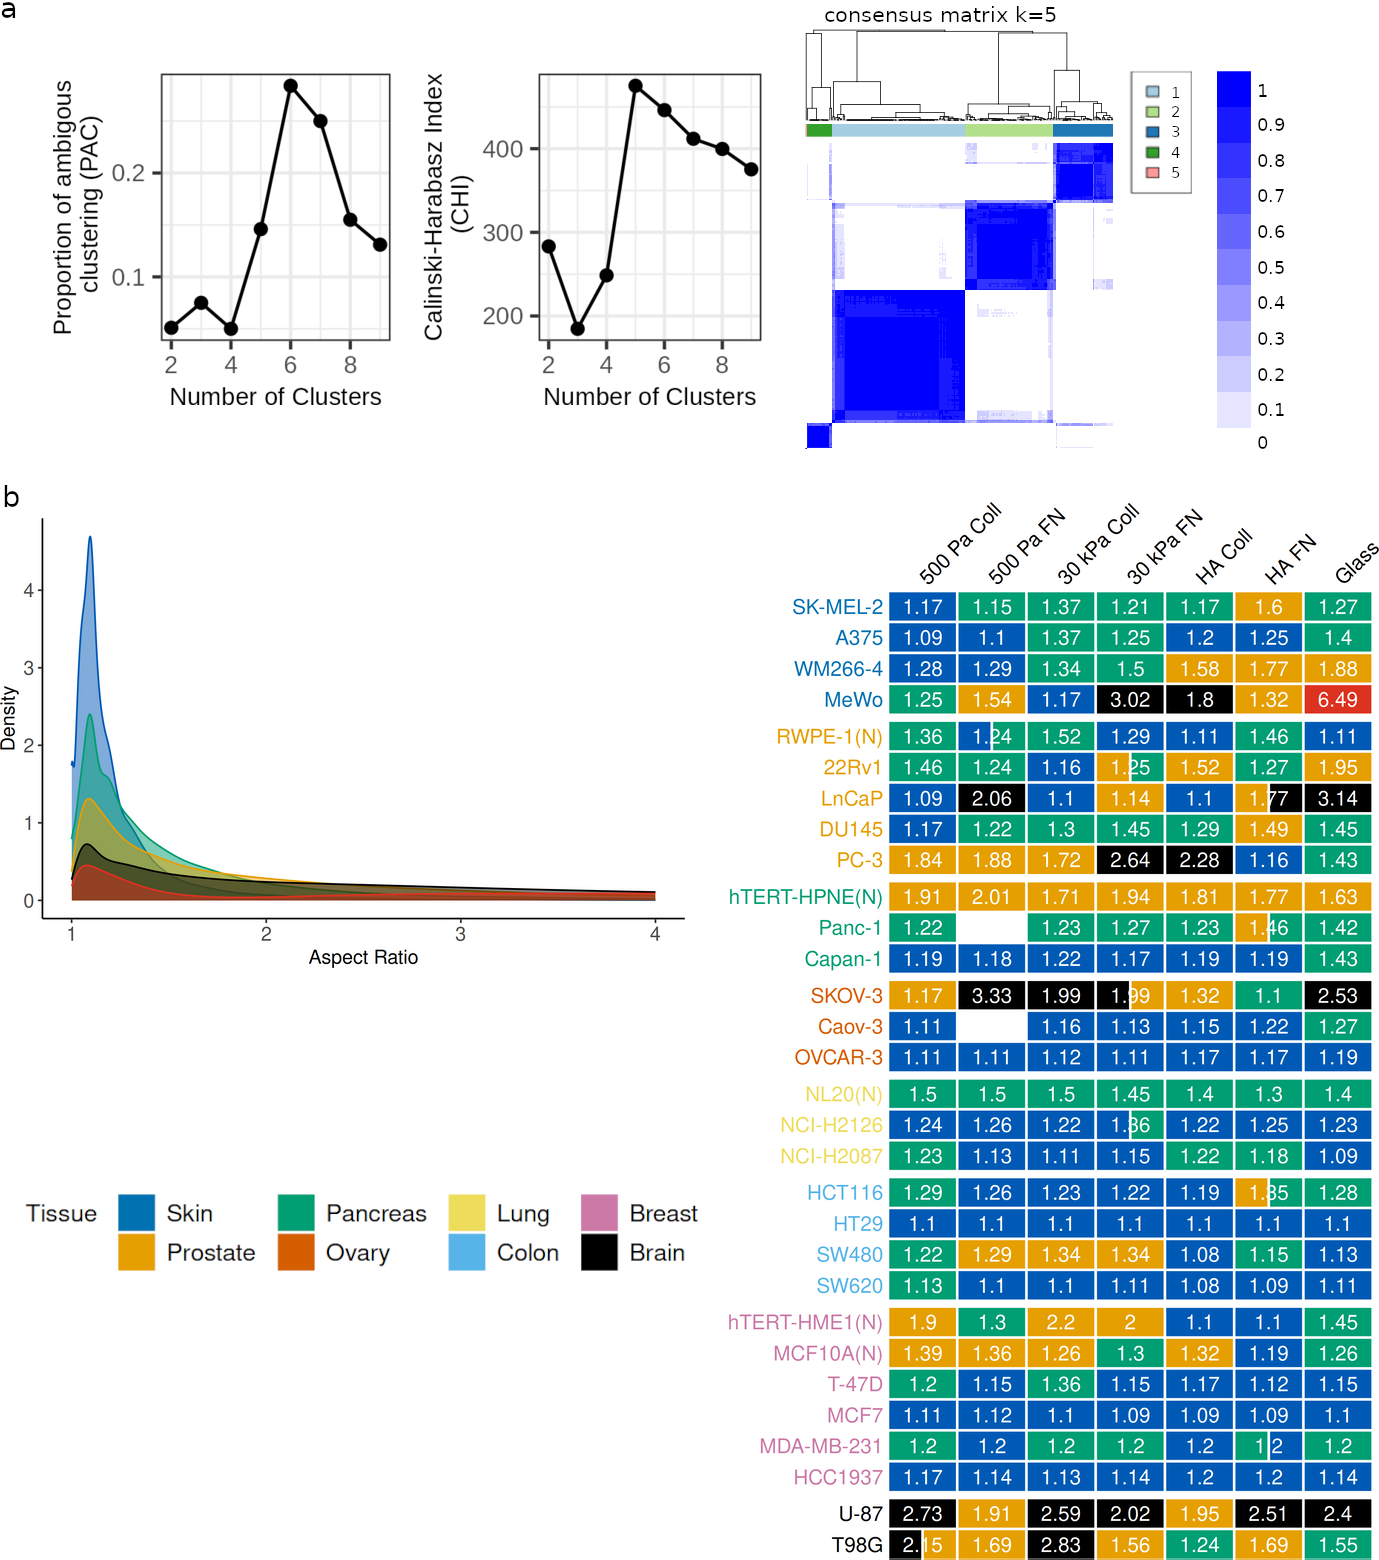
\includegraphics{../Figures/Supplementary_Figure12/supplementary_figure12.png}
    \caption{(a) Clustering statistics (PAC and CHI) used for identifying the optimal number of clusters (mechanotypes) based on Wasserstein-1 distance and the corresponding consensus matrix for optimal cluster count $k$
    of circularity. (b) Mechanotypes for aspect ratio, whereby the heatmap shows the phenotypic class for each cell line-substrate pair and the KDEs correspond to characteristic density function for each class. 
    The numeric values shown in the heatmap correspond to median values of circularity for each cell line-substrate pair. (N) refers to non-malignant (normal) cell lines. 
    Note that in this analysis only those cell line-substrate pairs are considered which have at least 25 data points $(n \geq 25)$ for the physical feature of interest.
    See supplementary tables 1 for the exact value of $n$ for the cell lines.}
    \label{fig:fig12}
\end{figure}

\begin{figure}[H]
    \centering
    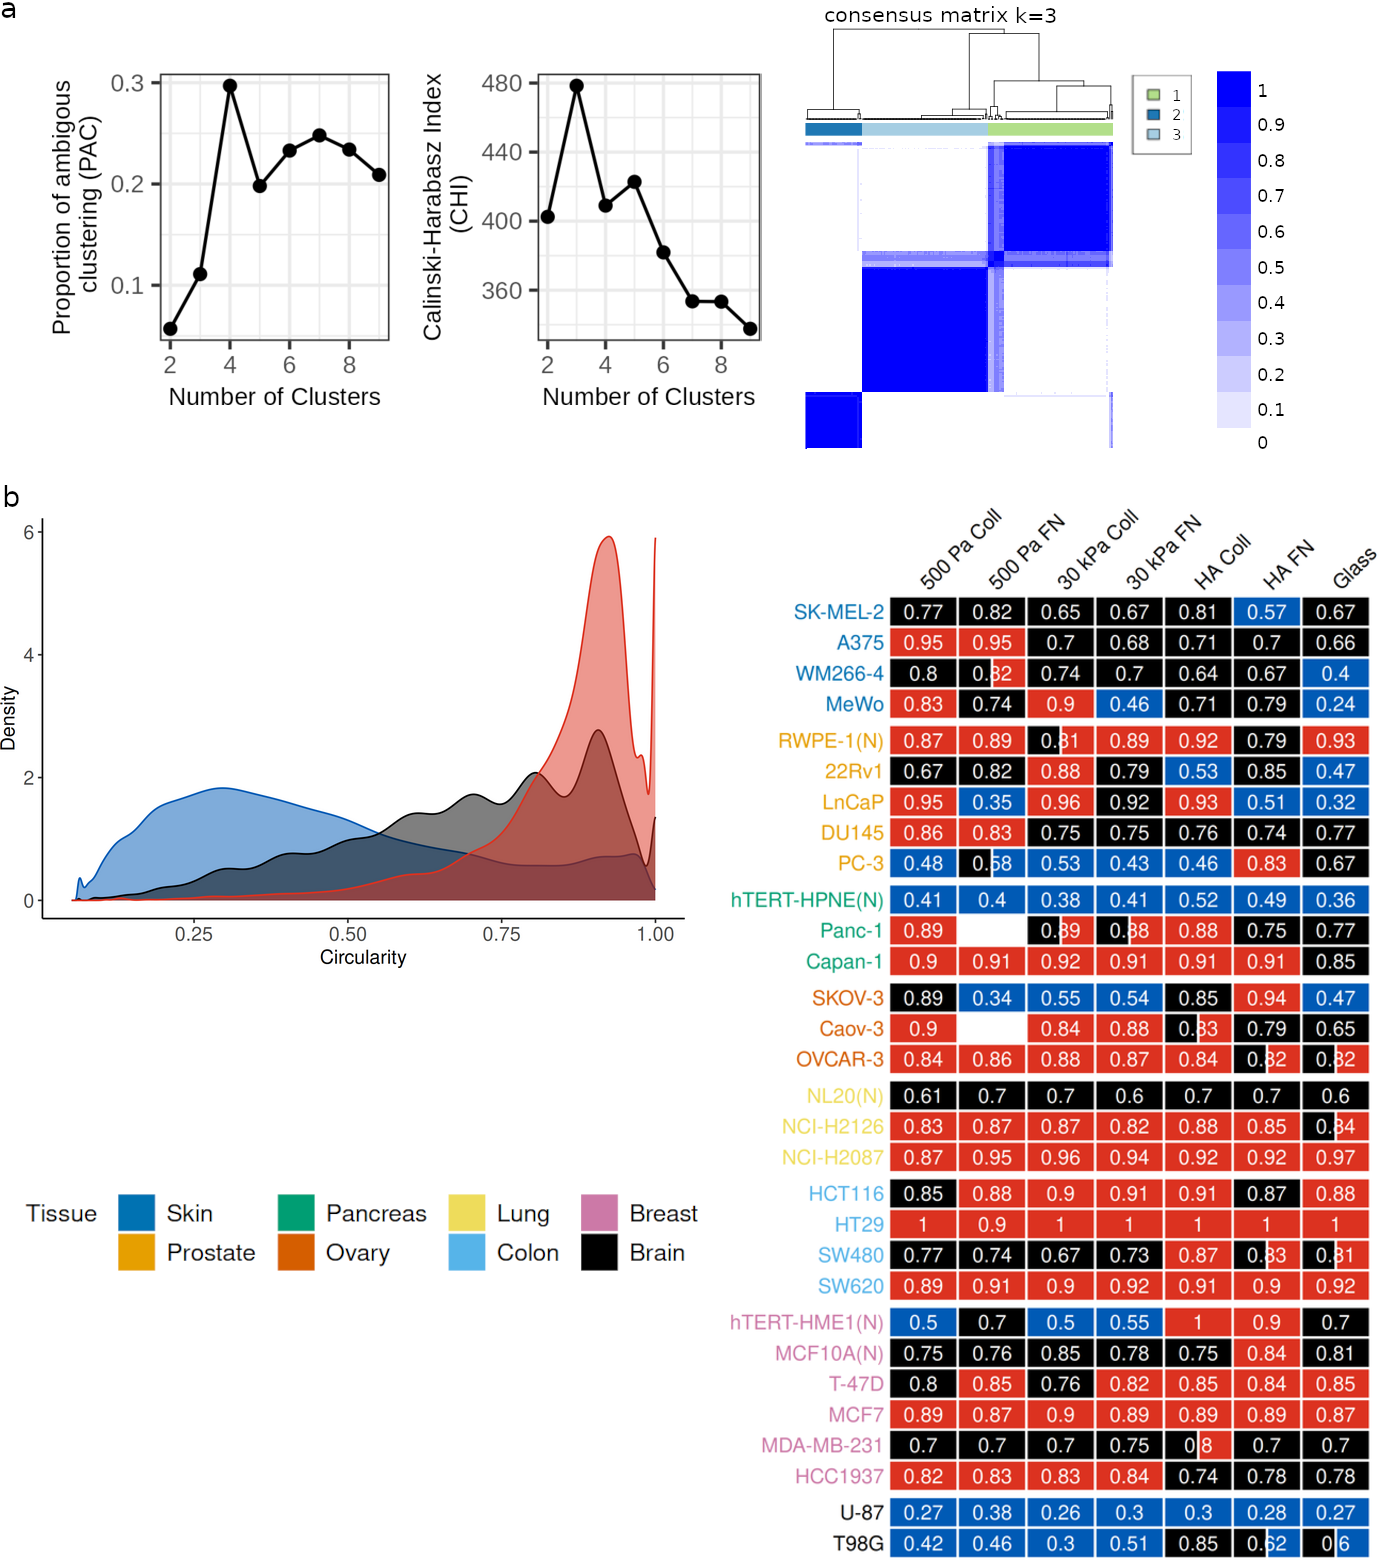
\includegraphics{../Figures/Supplementary_Figure13/supplementary_figure13.png}
    \caption{(a) Clustering statistics (PAC and CHI) used for identifying the optimal number of clusters (mechanotypes) based on Wasserstein-1 distance and the corresponding consensus matrix for optimal cluster count $k$
    of circularity. (b) Mechanotypes for circularity, whereby the heatmap shows the phenotypic class for each cell line-substrate pair and the KDEs correspond to characteristic density function for each class. 
    The numeric values shown in the heatmap correspond to median values of circularity for each cell line-substrate pair. (N) refers to non-malignant (normal) cell lines. 
    Note that in this analysis only those cell line-substrate pairs  are considered which have at least 25 data points $(n \geq 25)$ for the physical feature of interest.
    See supplementary tables 1 for the exact value of $n$ for the cell lines.}
    \label{fig:fig13}
\end{figure}

\begin{figure}[H]
    \centering
    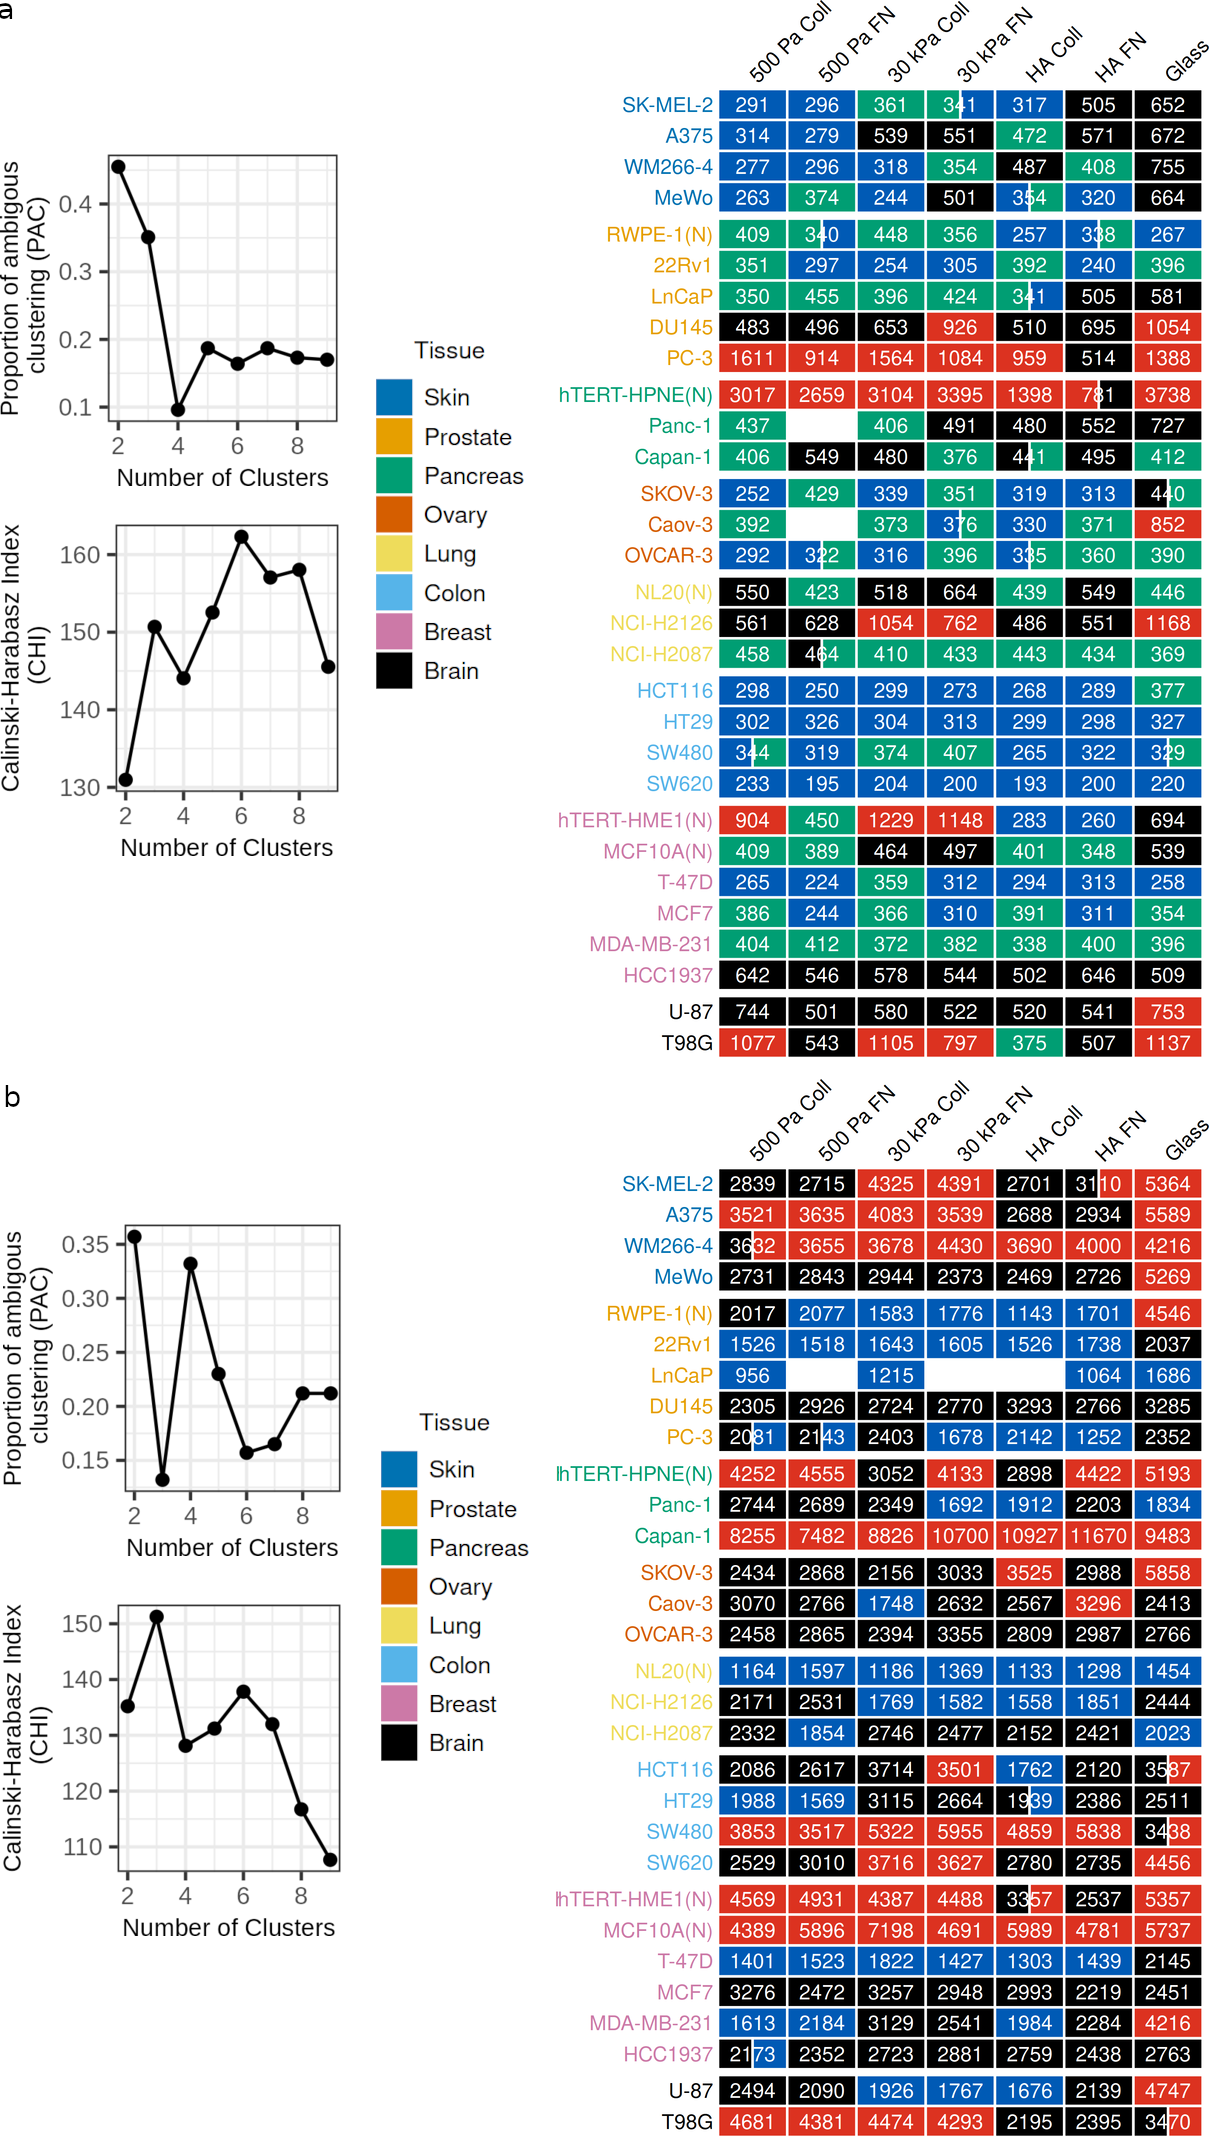
\includegraphics{../Figures/Supplementary_Figure14/supplementary_figure14.png}
    \caption{Clustering statistics (PAC and CHI) used for identifying the optimal number of clusters based on Kolomogrov-Smirnov distance and 
    the heatmap showing the corresponding classes for each of the cell line-substrate pairs for cell (a) area, and (b) stiffness. 
    The numeric values shown in the heatmap correspond to median values of circularity for each cell line-substrate pair. (N) refers to non-malignant (normal) cell lines. 
    Note that in this analysis only those cell line-substrate pairs are considered which have at least 25 data points $(n \geq 25)$ for the physical feature of interest.
    See supplementary tables 1 and 2 for the exact value of $n$ for the cell lines.}
    \label{fig:fig14}
\end{figure}

\begin{figure}[H]
    \hspace*{-0.8cm}
    \centering
    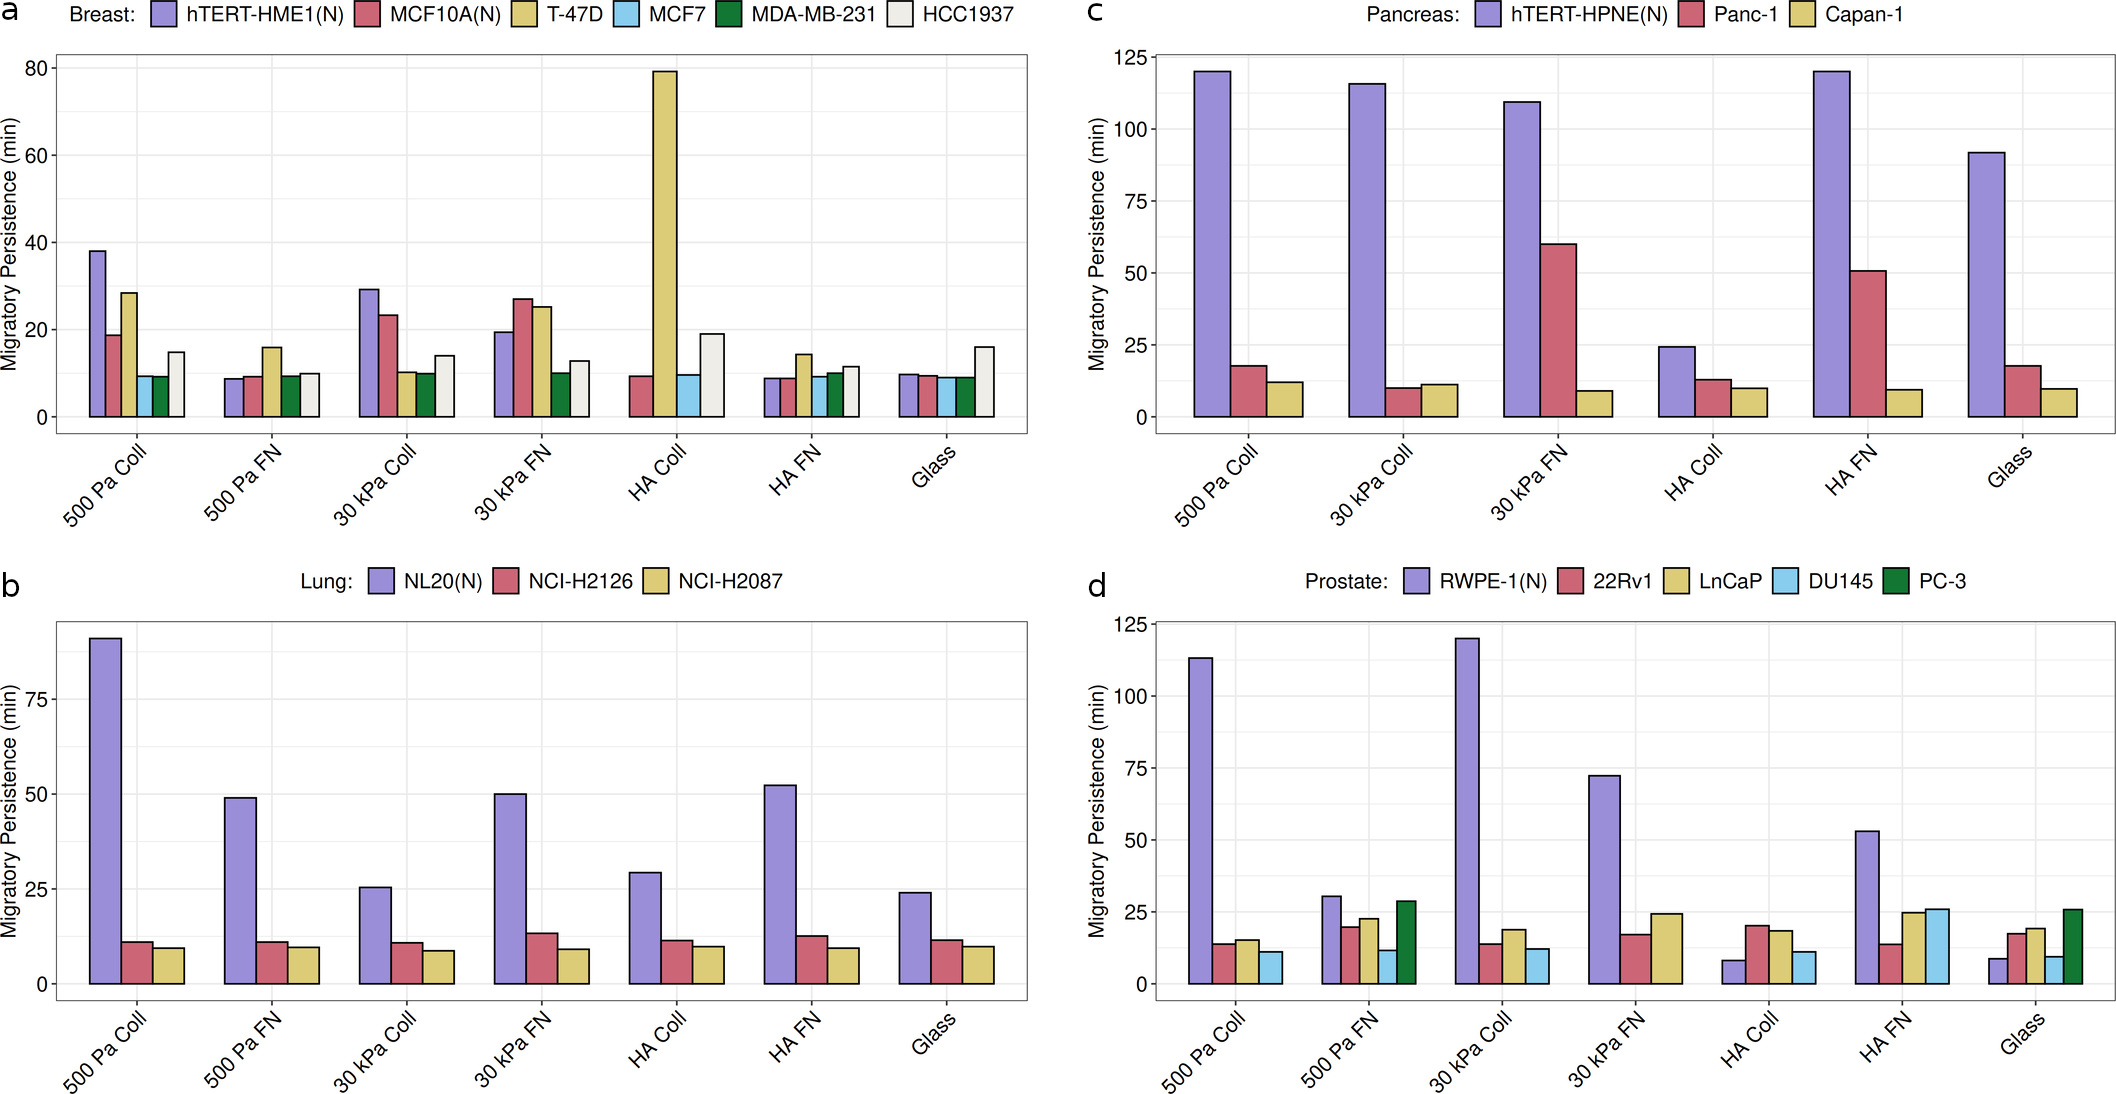
\includegraphics{../Figures/Supplementary_Figure15/supplementary_figure15.png}
    \caption{Comparison between tissue-specific normal and cancer cell behavior in terms of migratory persistence for (a) breast, (b) lung, (c) pancreas, and (c) prostate cell lines.
    (N) refers to non-malignant (normal) cell lines. 
    Decorrelation time estimated from directional autocorrelation curves (shown in Supp. Fig. 18-20) is used as a measure of migratory persistence.
    Note that, for RWPE-1 cell line on 30 kPa Coll, hTERT-HPNE cell line on 500 Pa Coll, 500 Pa FN and HA FN, and Panc-1 cell line on 30 kPa FN,
    the directional autocorrelation did not fall below 0.2 cutoff used to determine decorrelation time.
    For these cases, the total trajectory time is used as a measure of migratory persistence.}
    \label{fig:fig15}
\end{figure}

\begin{figure}[H]
    \centering
    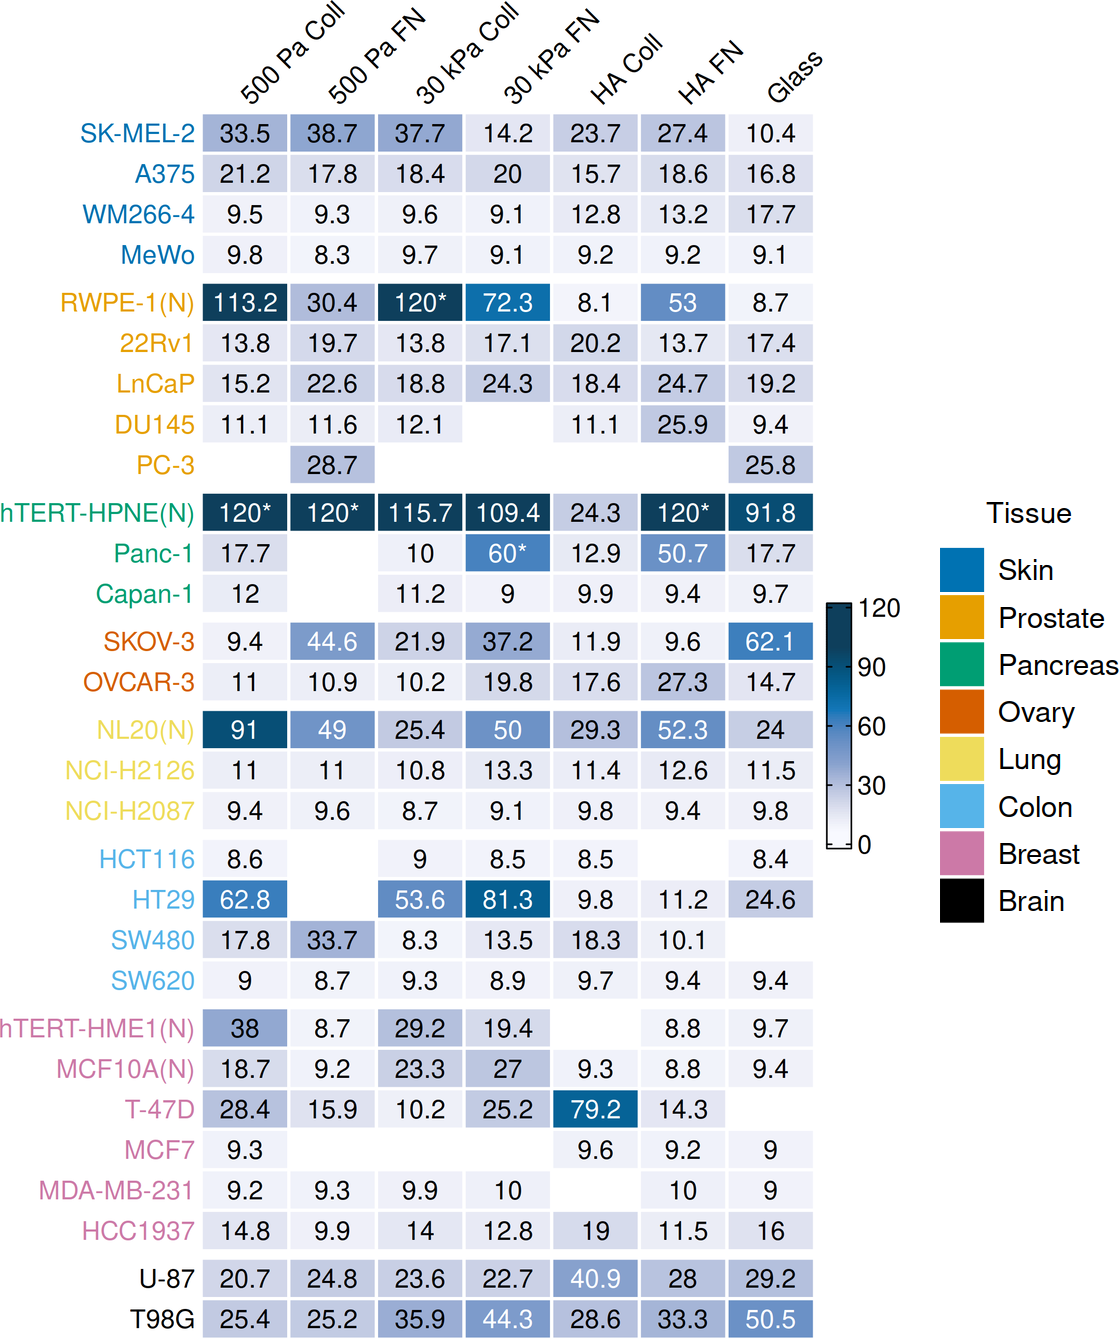
\includegraphics{../Figures/Supplementary_Figure16/supplementary_figure16.png}
    \caption{Heatmap showing the migratory persistence for each of the cell line-substrate pairs. 
    (N) refers to non-malignant (normal) cell lines. 
    Decorrelation time estimated from directional autocorrelation curves (shown in Supp. Fig. 17-21) is used as a measure of migratory persistence.
    Note that (*) represents the cell line-substrate pairs for which the directional autocorrelation did not fall below 0.2 cutoff used to determine 
    decorrelation time. For these cases, the total trajectory time is used as a measure of migratory persistence.} 
    \label{fig:fig16}
\end{figure}

\begin{figure}[H]
    \hspace*{-0.8cm}
    \centering
    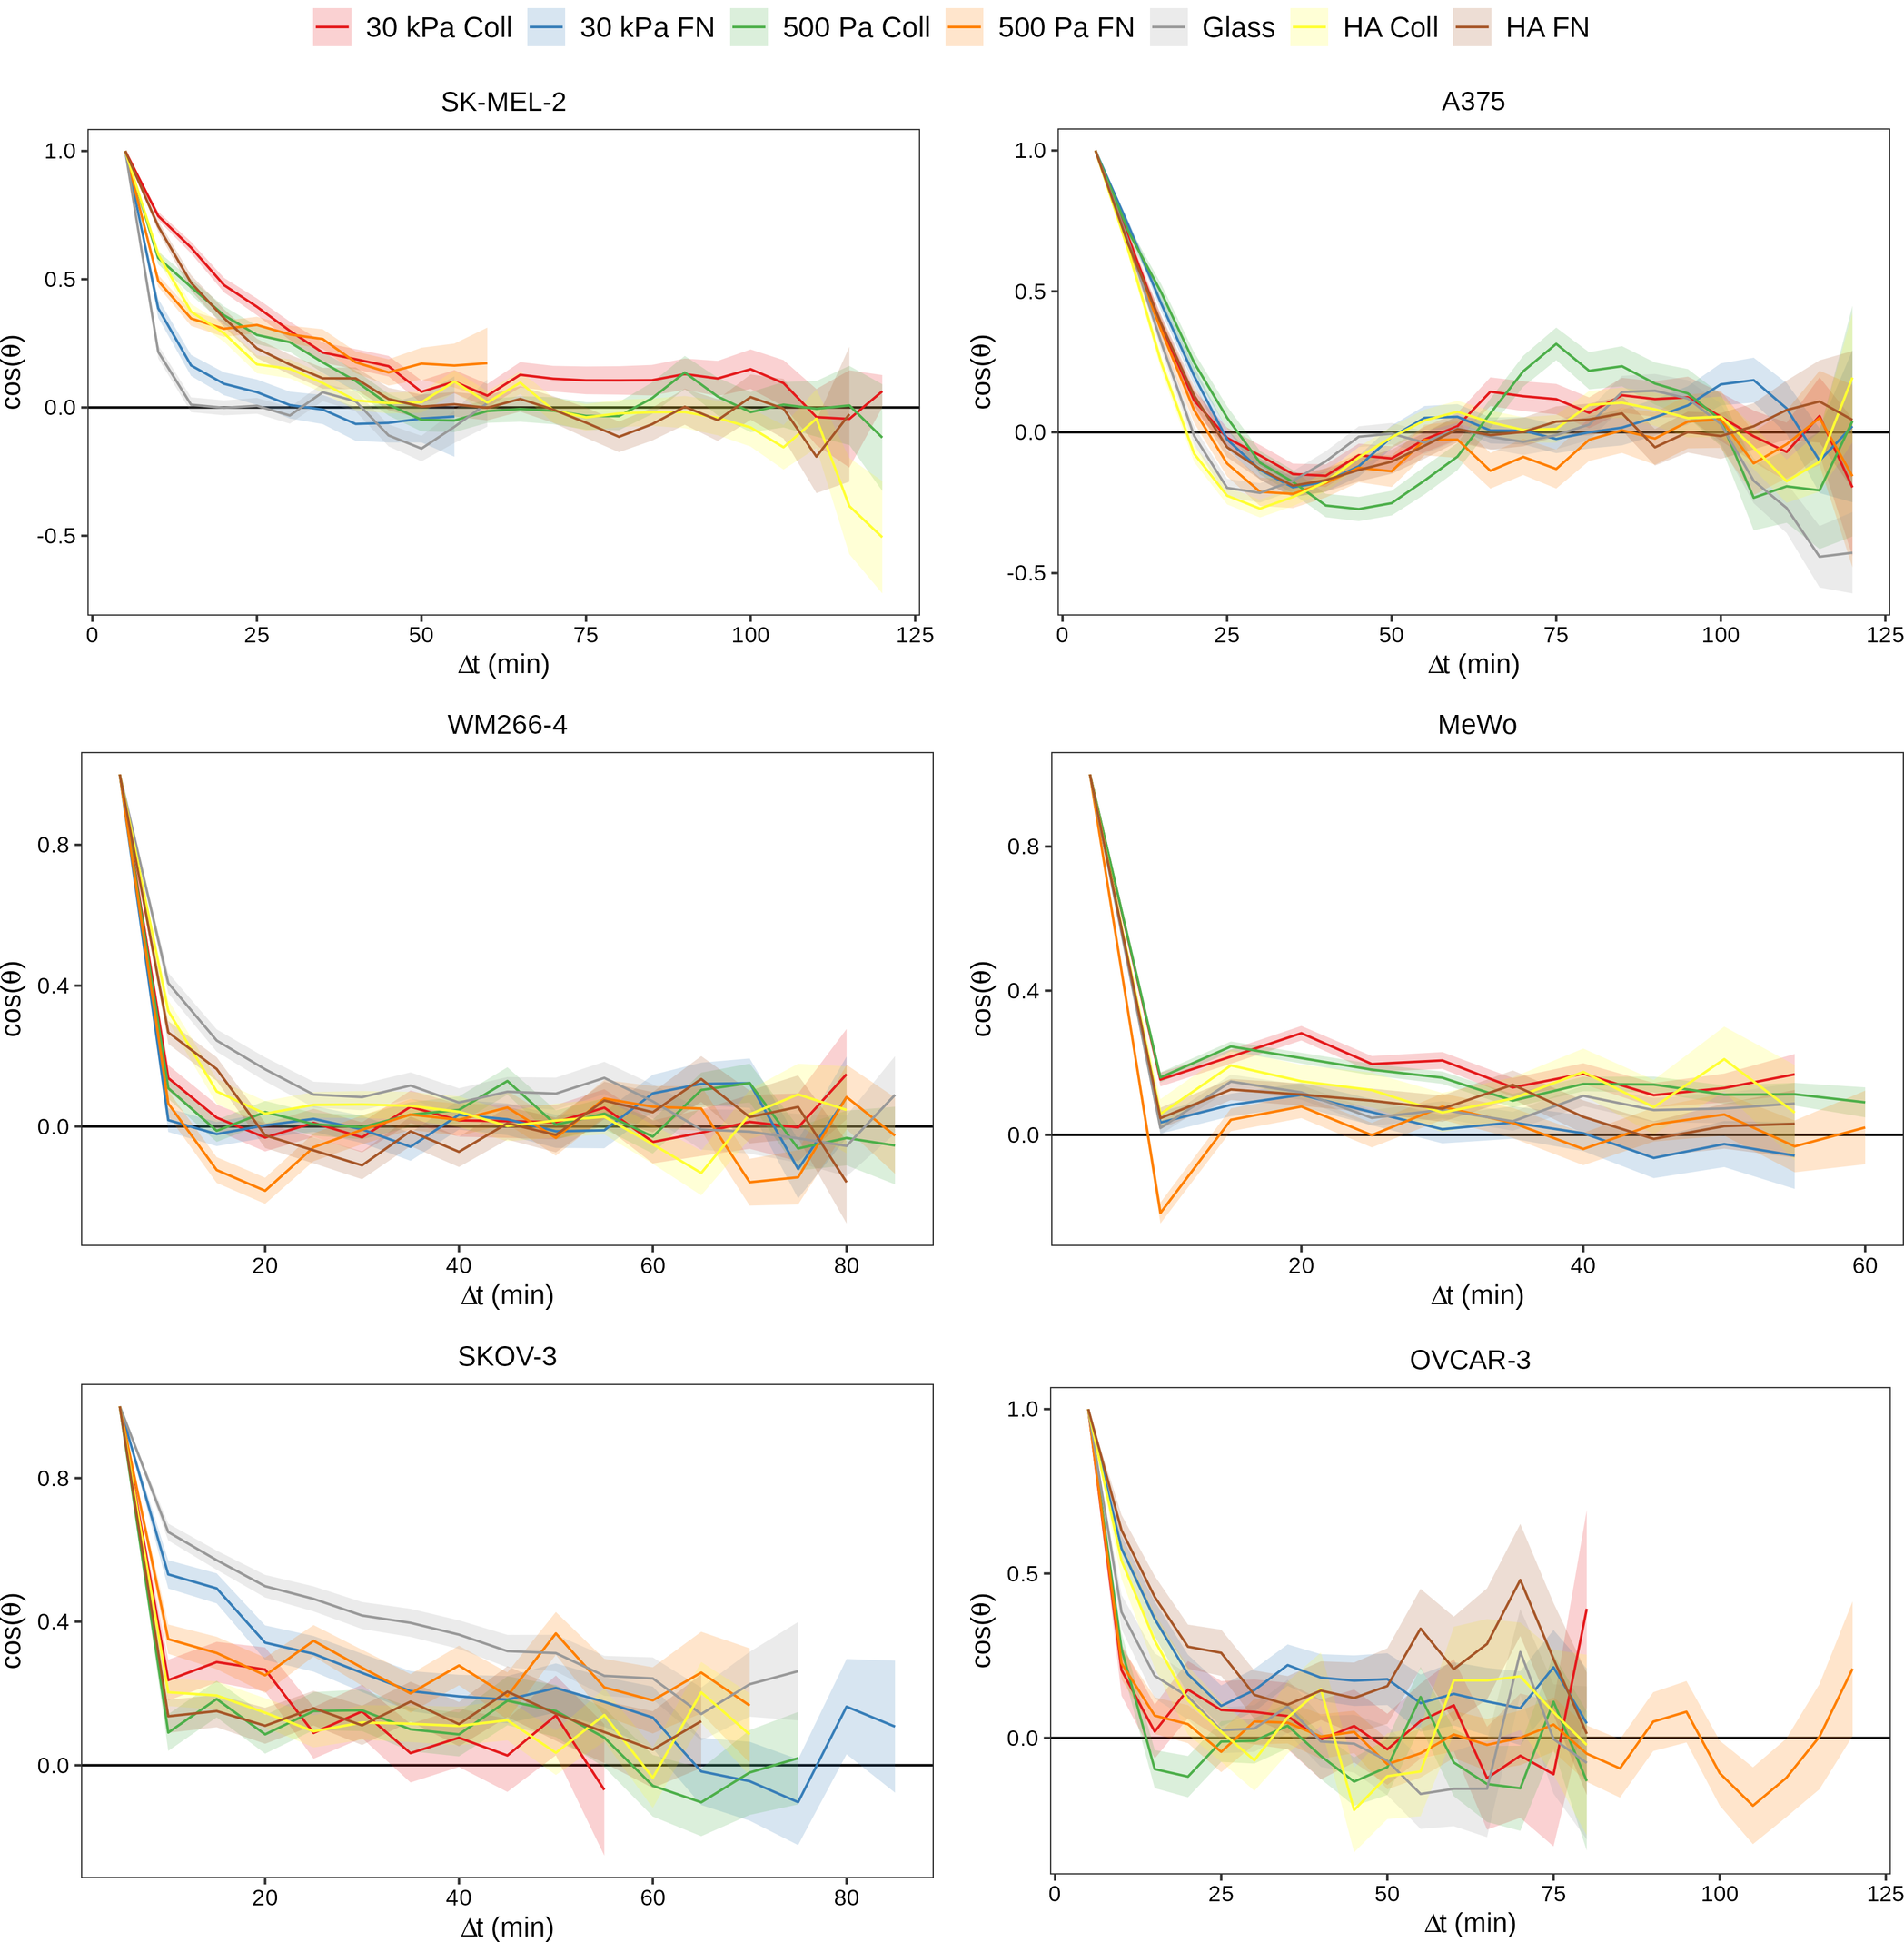
\includegraphics{../Figures/Supplementary_Figures17_21/supplementary_figure17.png}
    \caption{Directional autocorrelation comparing the persistence of cell migration for cell lines on different substrates.
    For each cell line, only those substrates are analysed that have $n \geq 25$ measurements.
    See supplementary tables 3 for the exact value of $n$ for the cell lines.}
    \label{fig:fig17}
\end{figure}

\begin{figure}[H]
    \hspace*{-0.8cm}
    \centering
    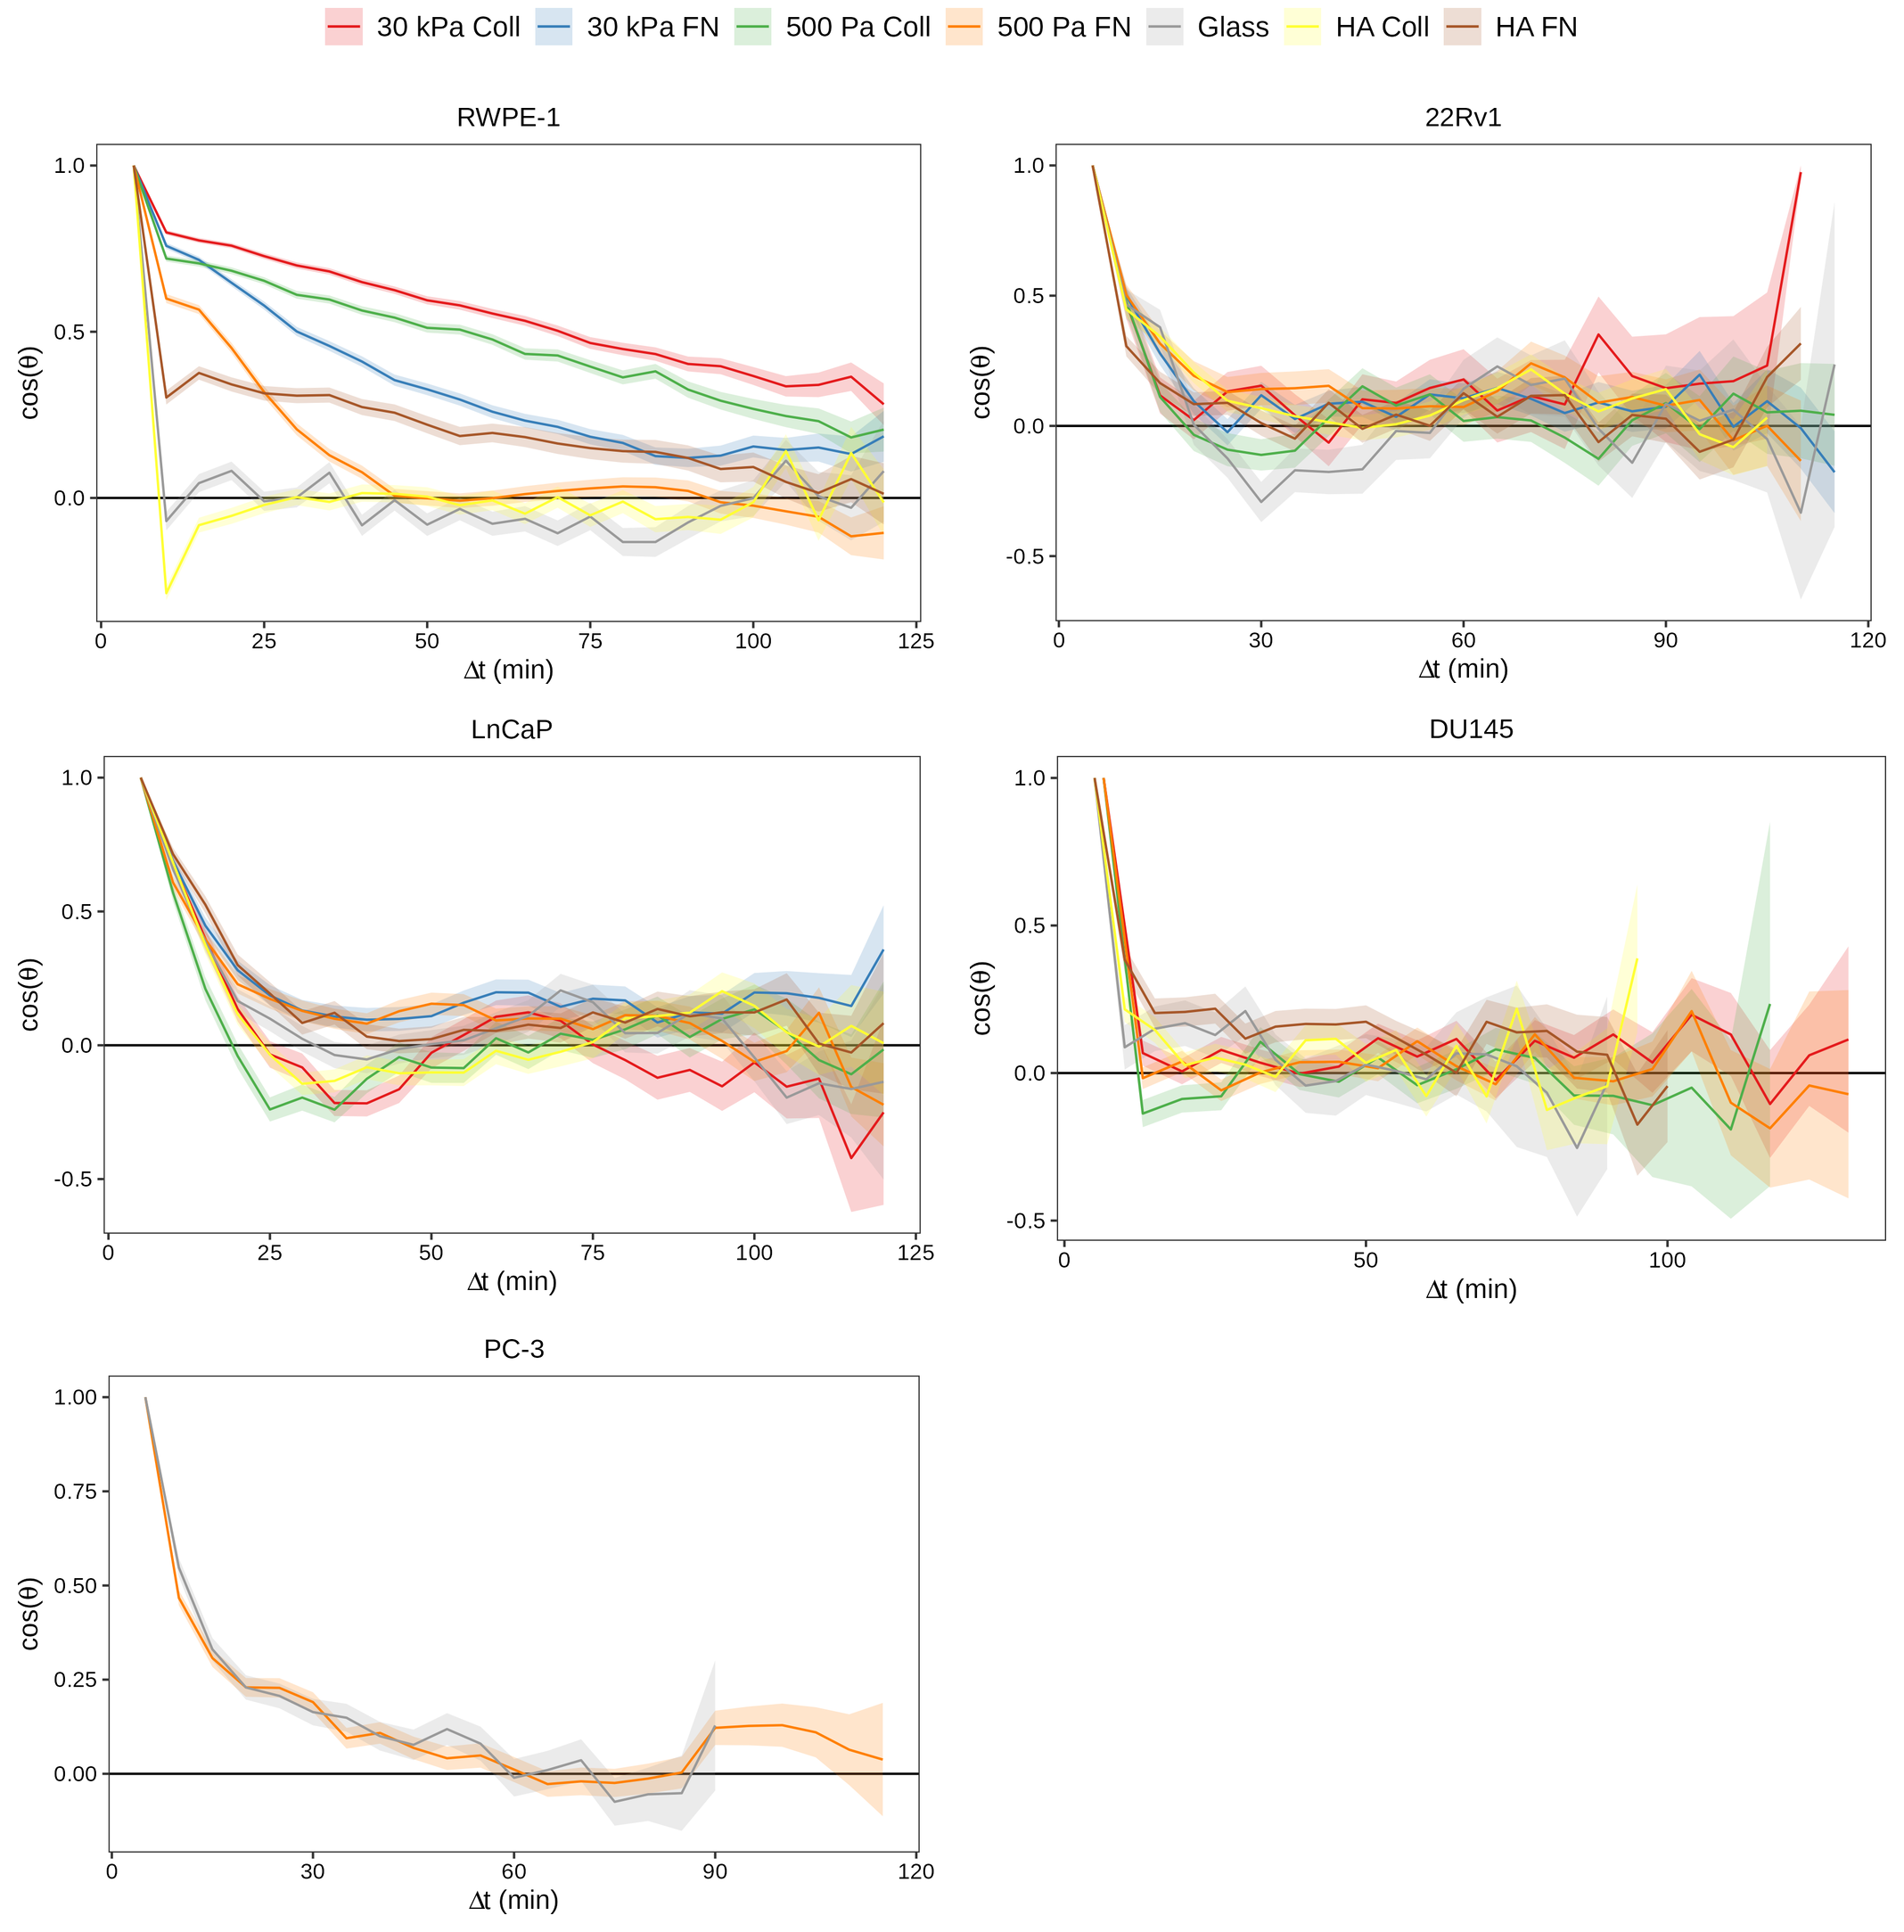
\includegraphics{../Figures/Supplementary_Figures17_21/supplementary_figure18.png}
    \caption{Directional autocorrelation comparing the persistence of cell migration for cell lines on different substrates.
    For each cell line, only those substrates are analysed that have $n \geq 25$ measurements.
    See supplementary tables 3 for the exact value of $n$ for the cell lines.}
    \label{fig:fig18}
\end{figure}

\begin{figure}[H]
    \hspace*{-0.8cm}
    \centering
    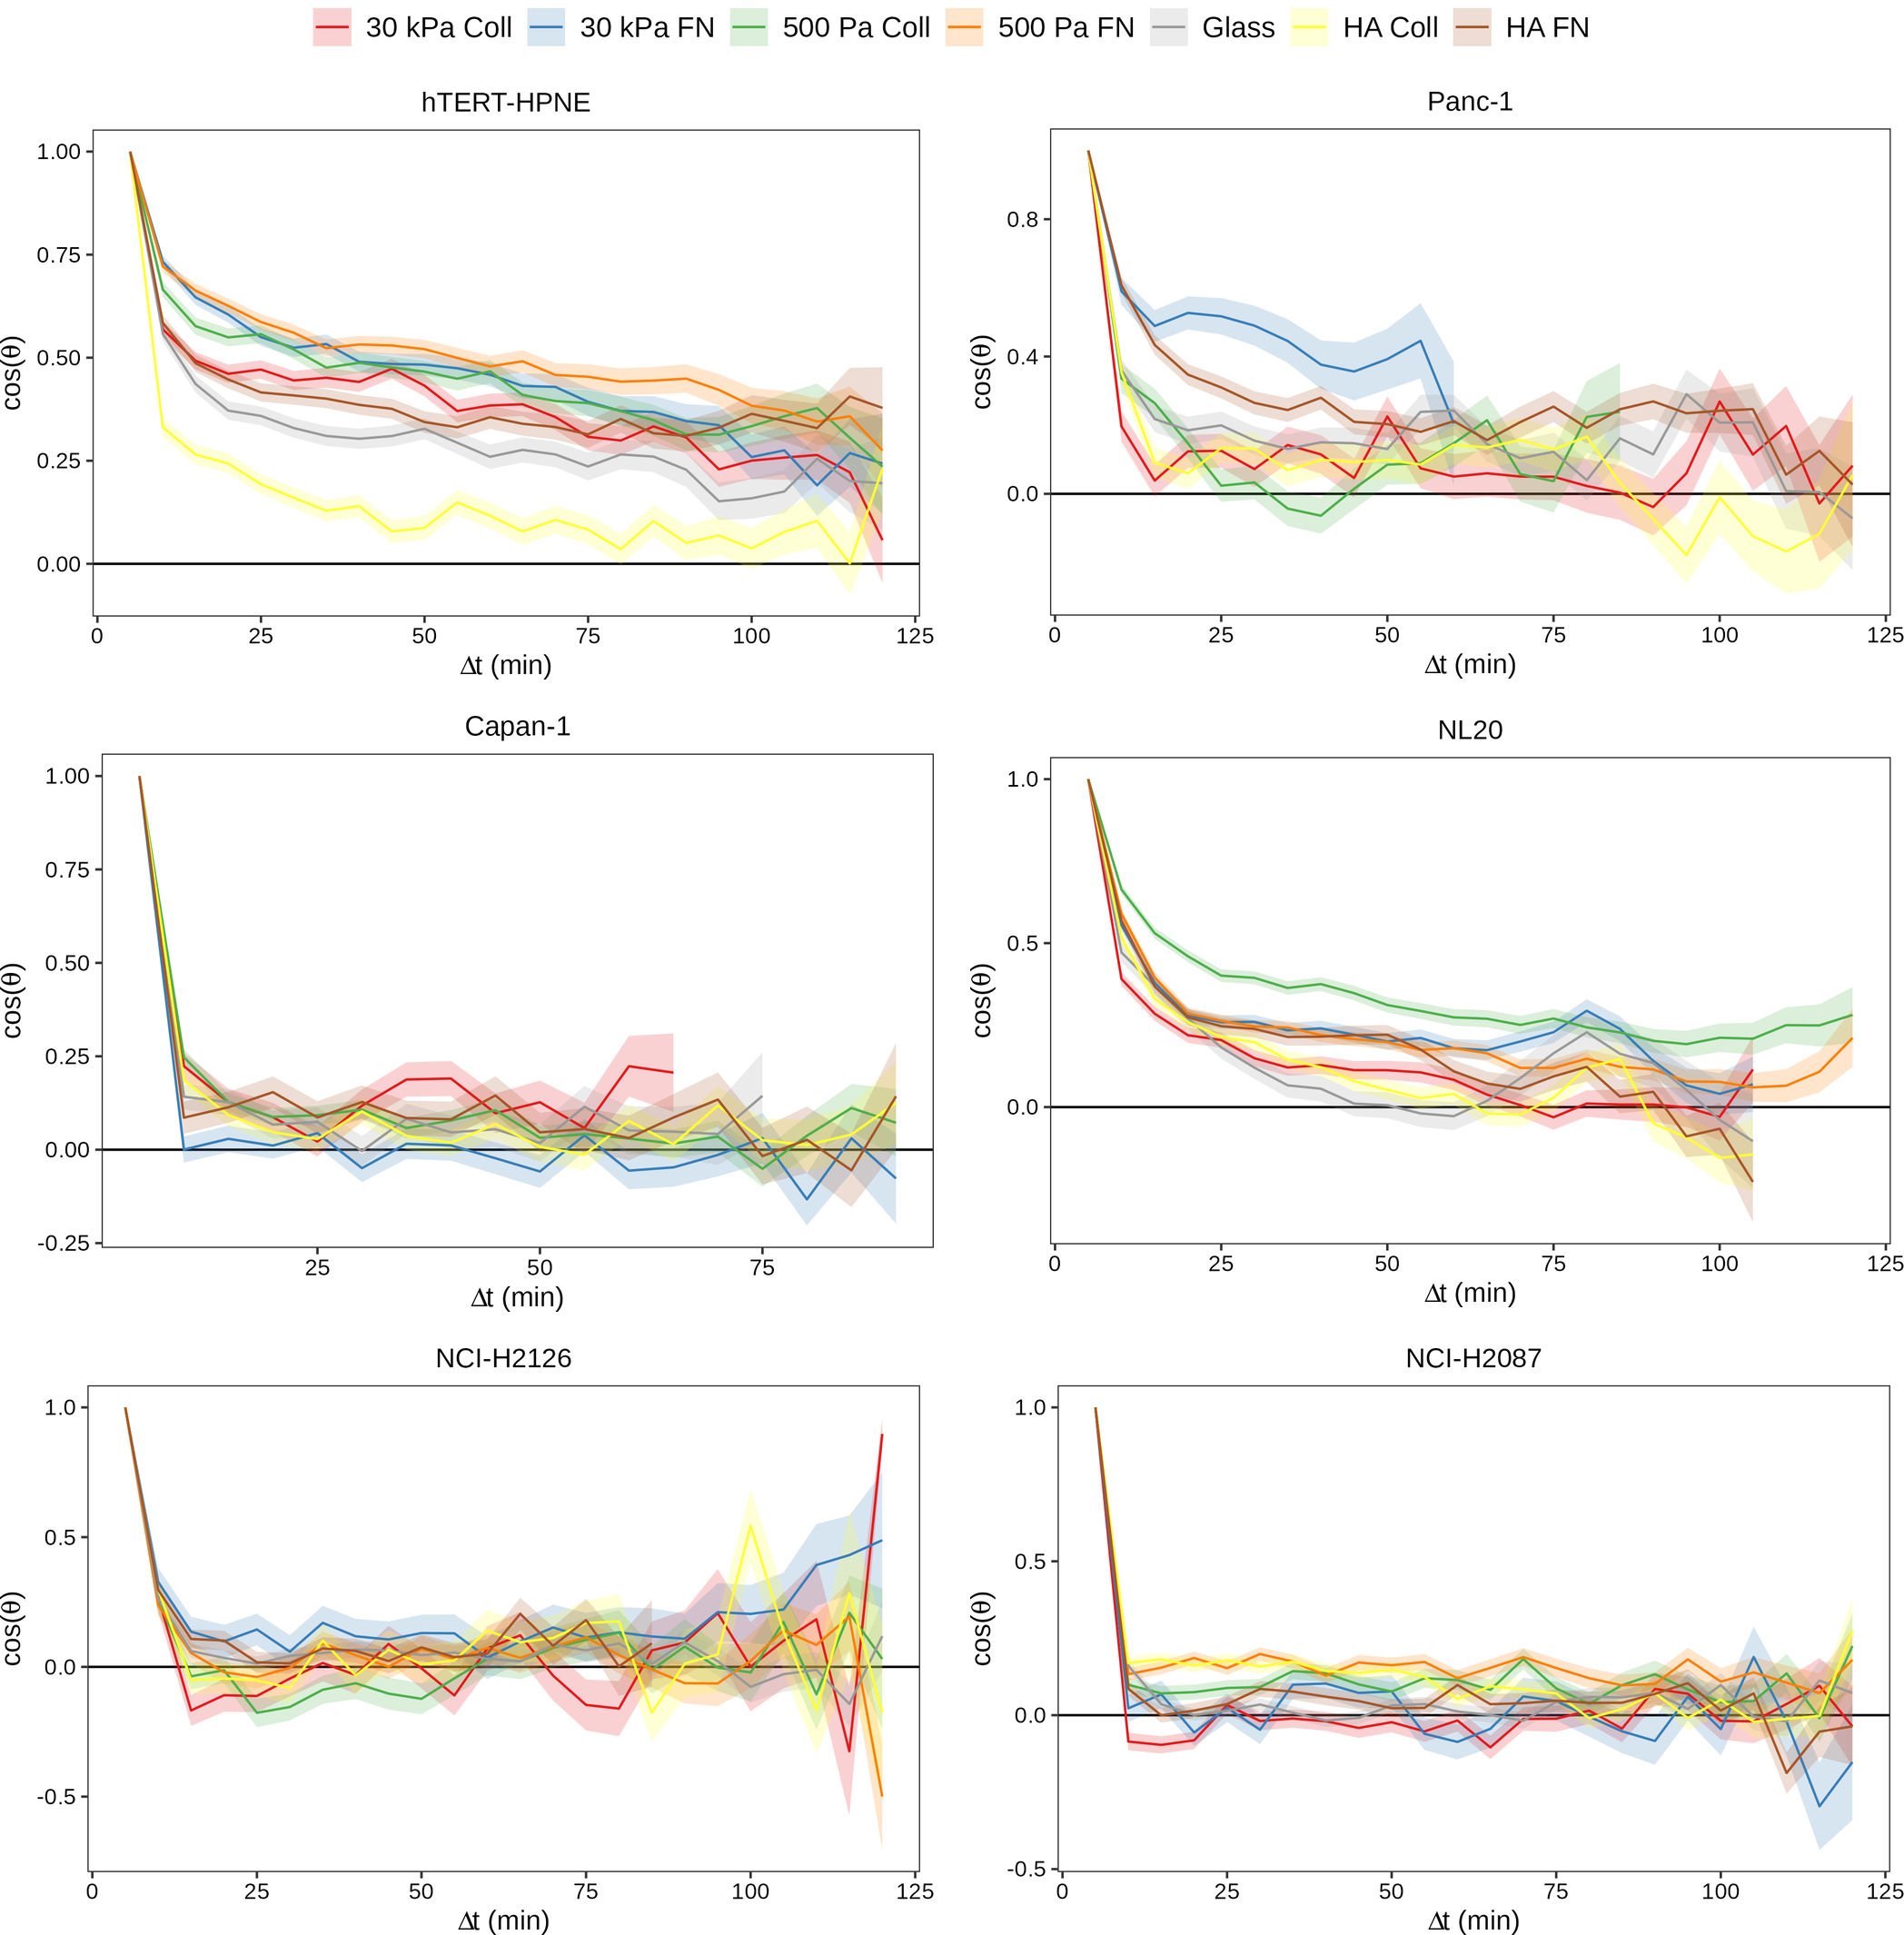
\includegraphics{../Figures/Supplementary_Figures17_21/supplementary_figure19.png}
    \caption{Directional autocorrelation comparing the persistence of cell migration for cell lines on different substrates.
    For each cell line, only those substrates are analysed that have $n \geq 25$ measurements.
    See supplementary tables 3 for the exact value of $n$ for the cell lines.}
    \label{fig:fig19}
\end{figure}

\begin{figure}[H]
    \hspace*{-0.8cm}
    \centering
    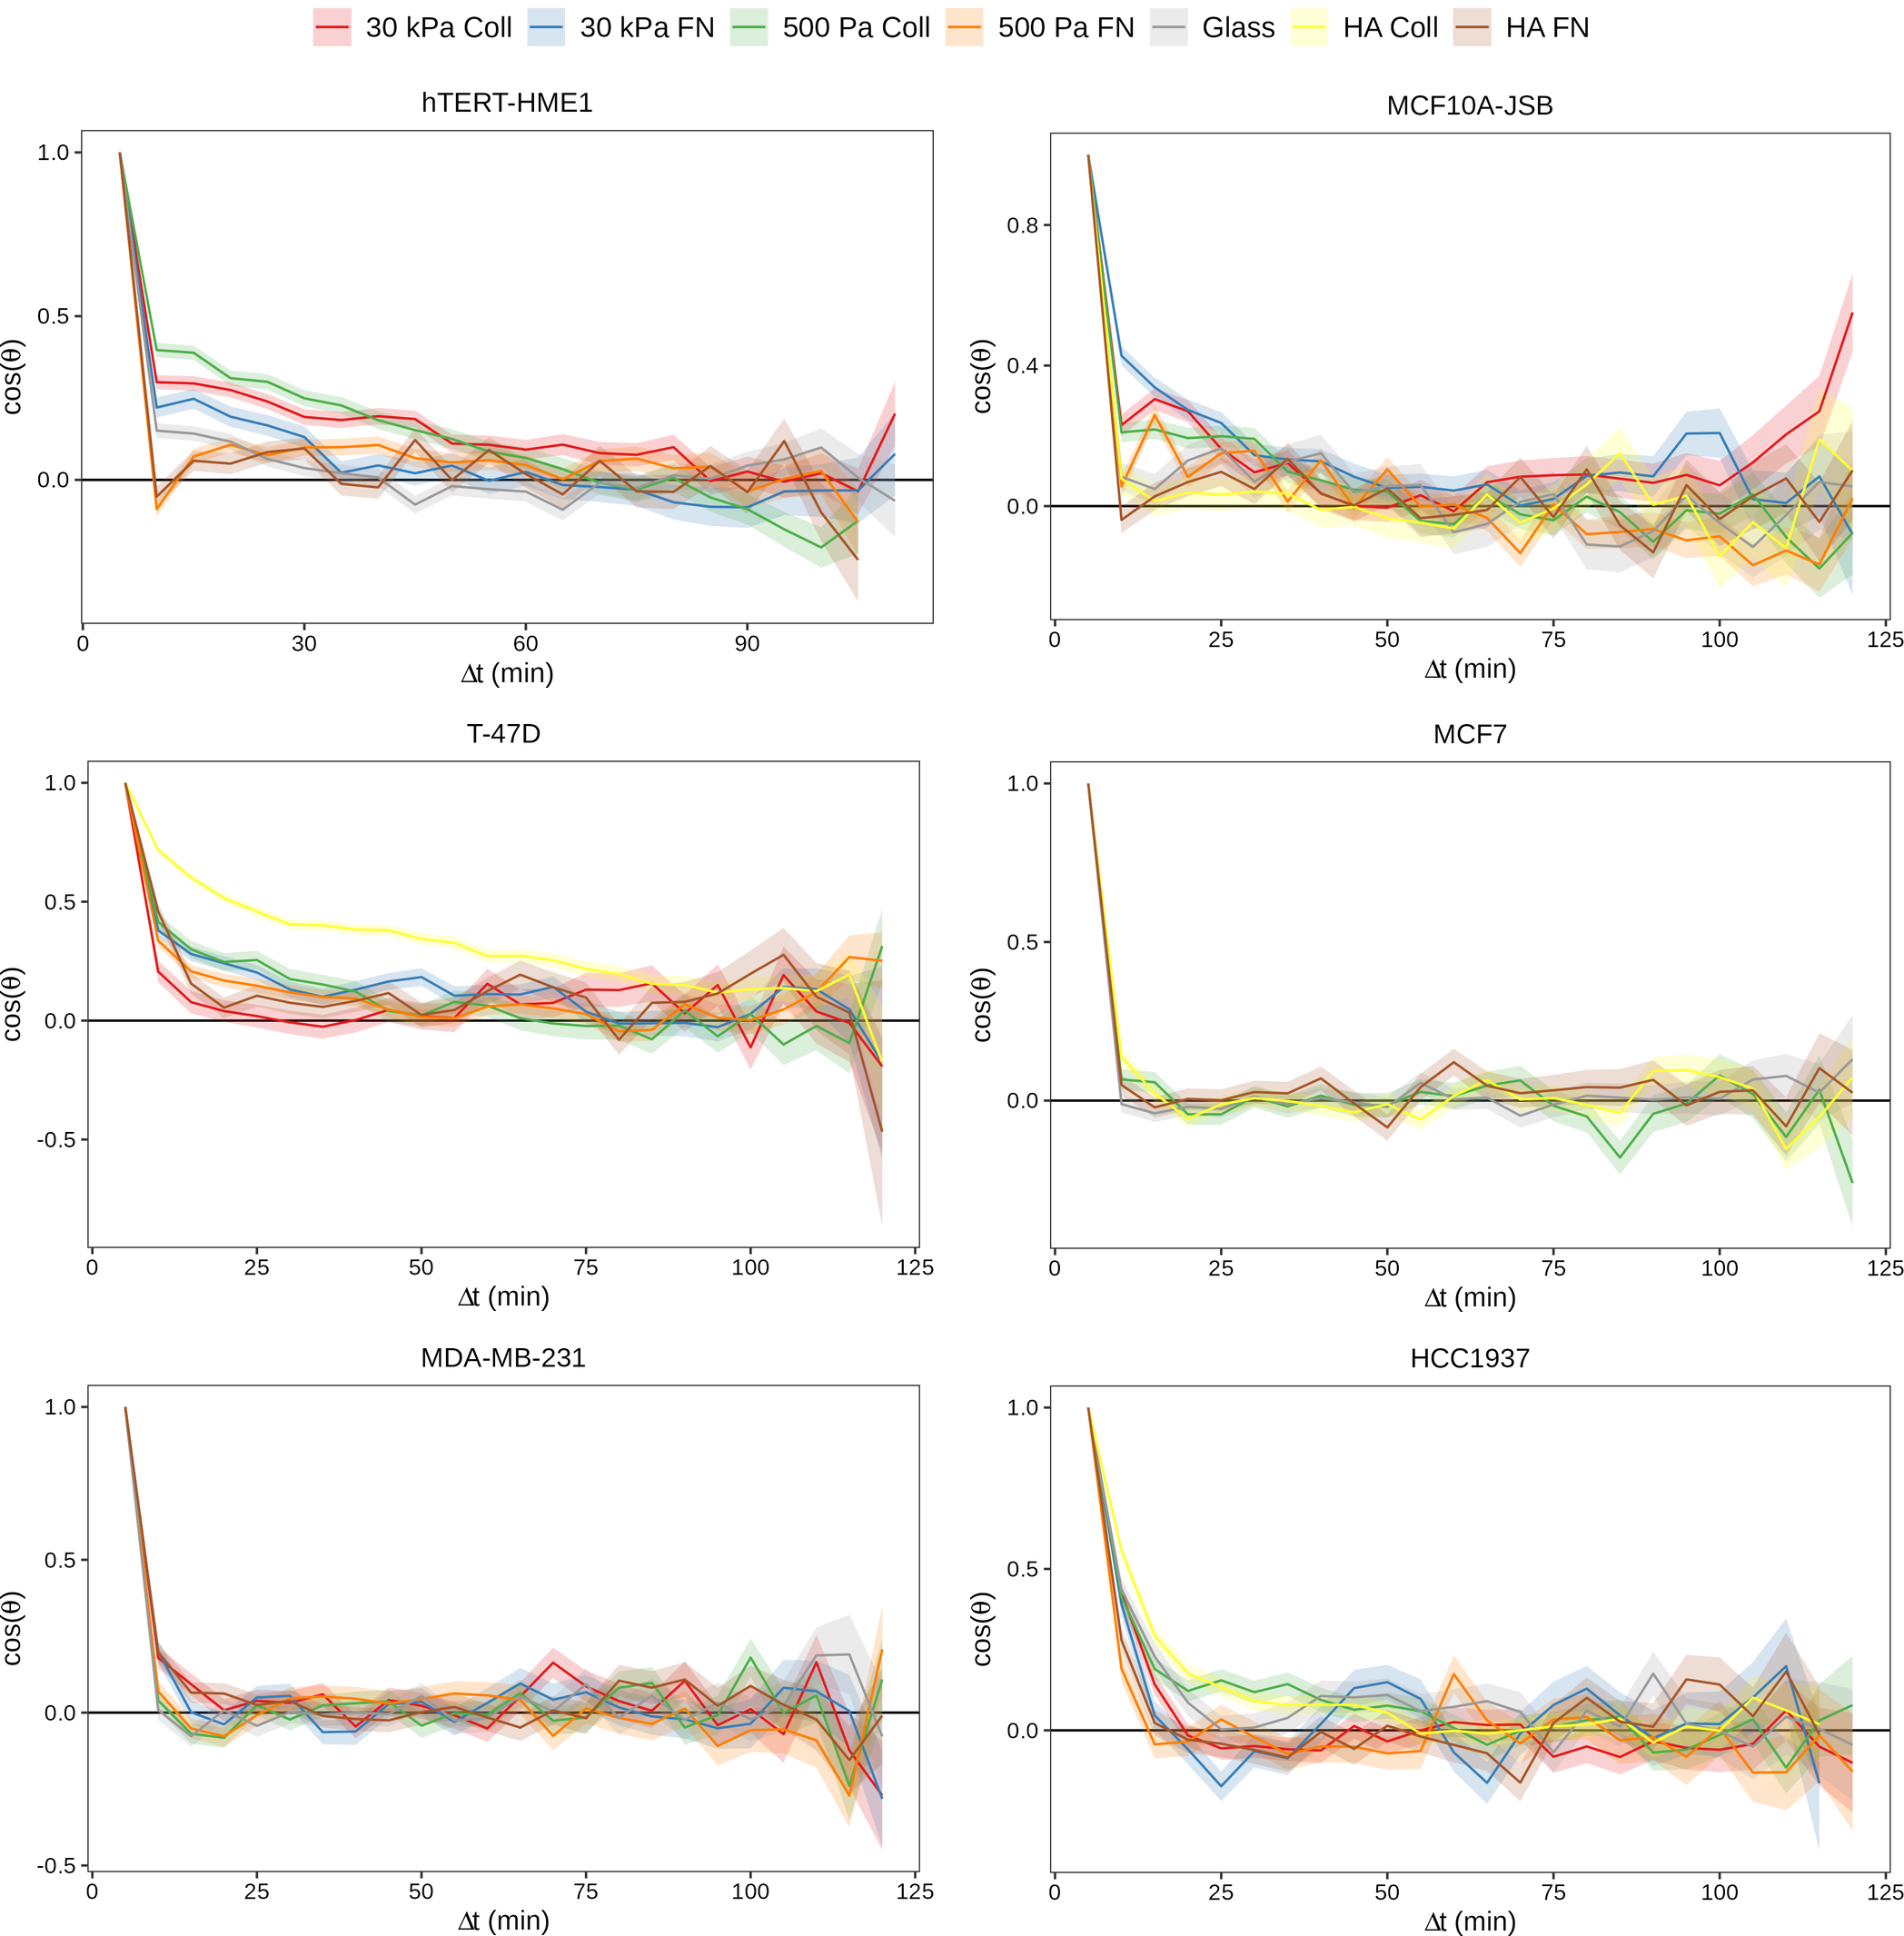
\includegraphics{../Figures/Supplementary_Figures17_21/supplementary_figure20.png}
    \caption{Directional autocorrelation comparing the persistence of cell migration for cell lines on different substrates.
    For each cell line, only those substrates are analysed that have $n \geq 25$ measurements.
    See supplementary tables 3 for the exact value of $n$ for the cell lines.}
    \label{fig:fig20}
\end{figure}

\begin{figure}[H]
    \hspace*{-0.8cm}
    \centering
    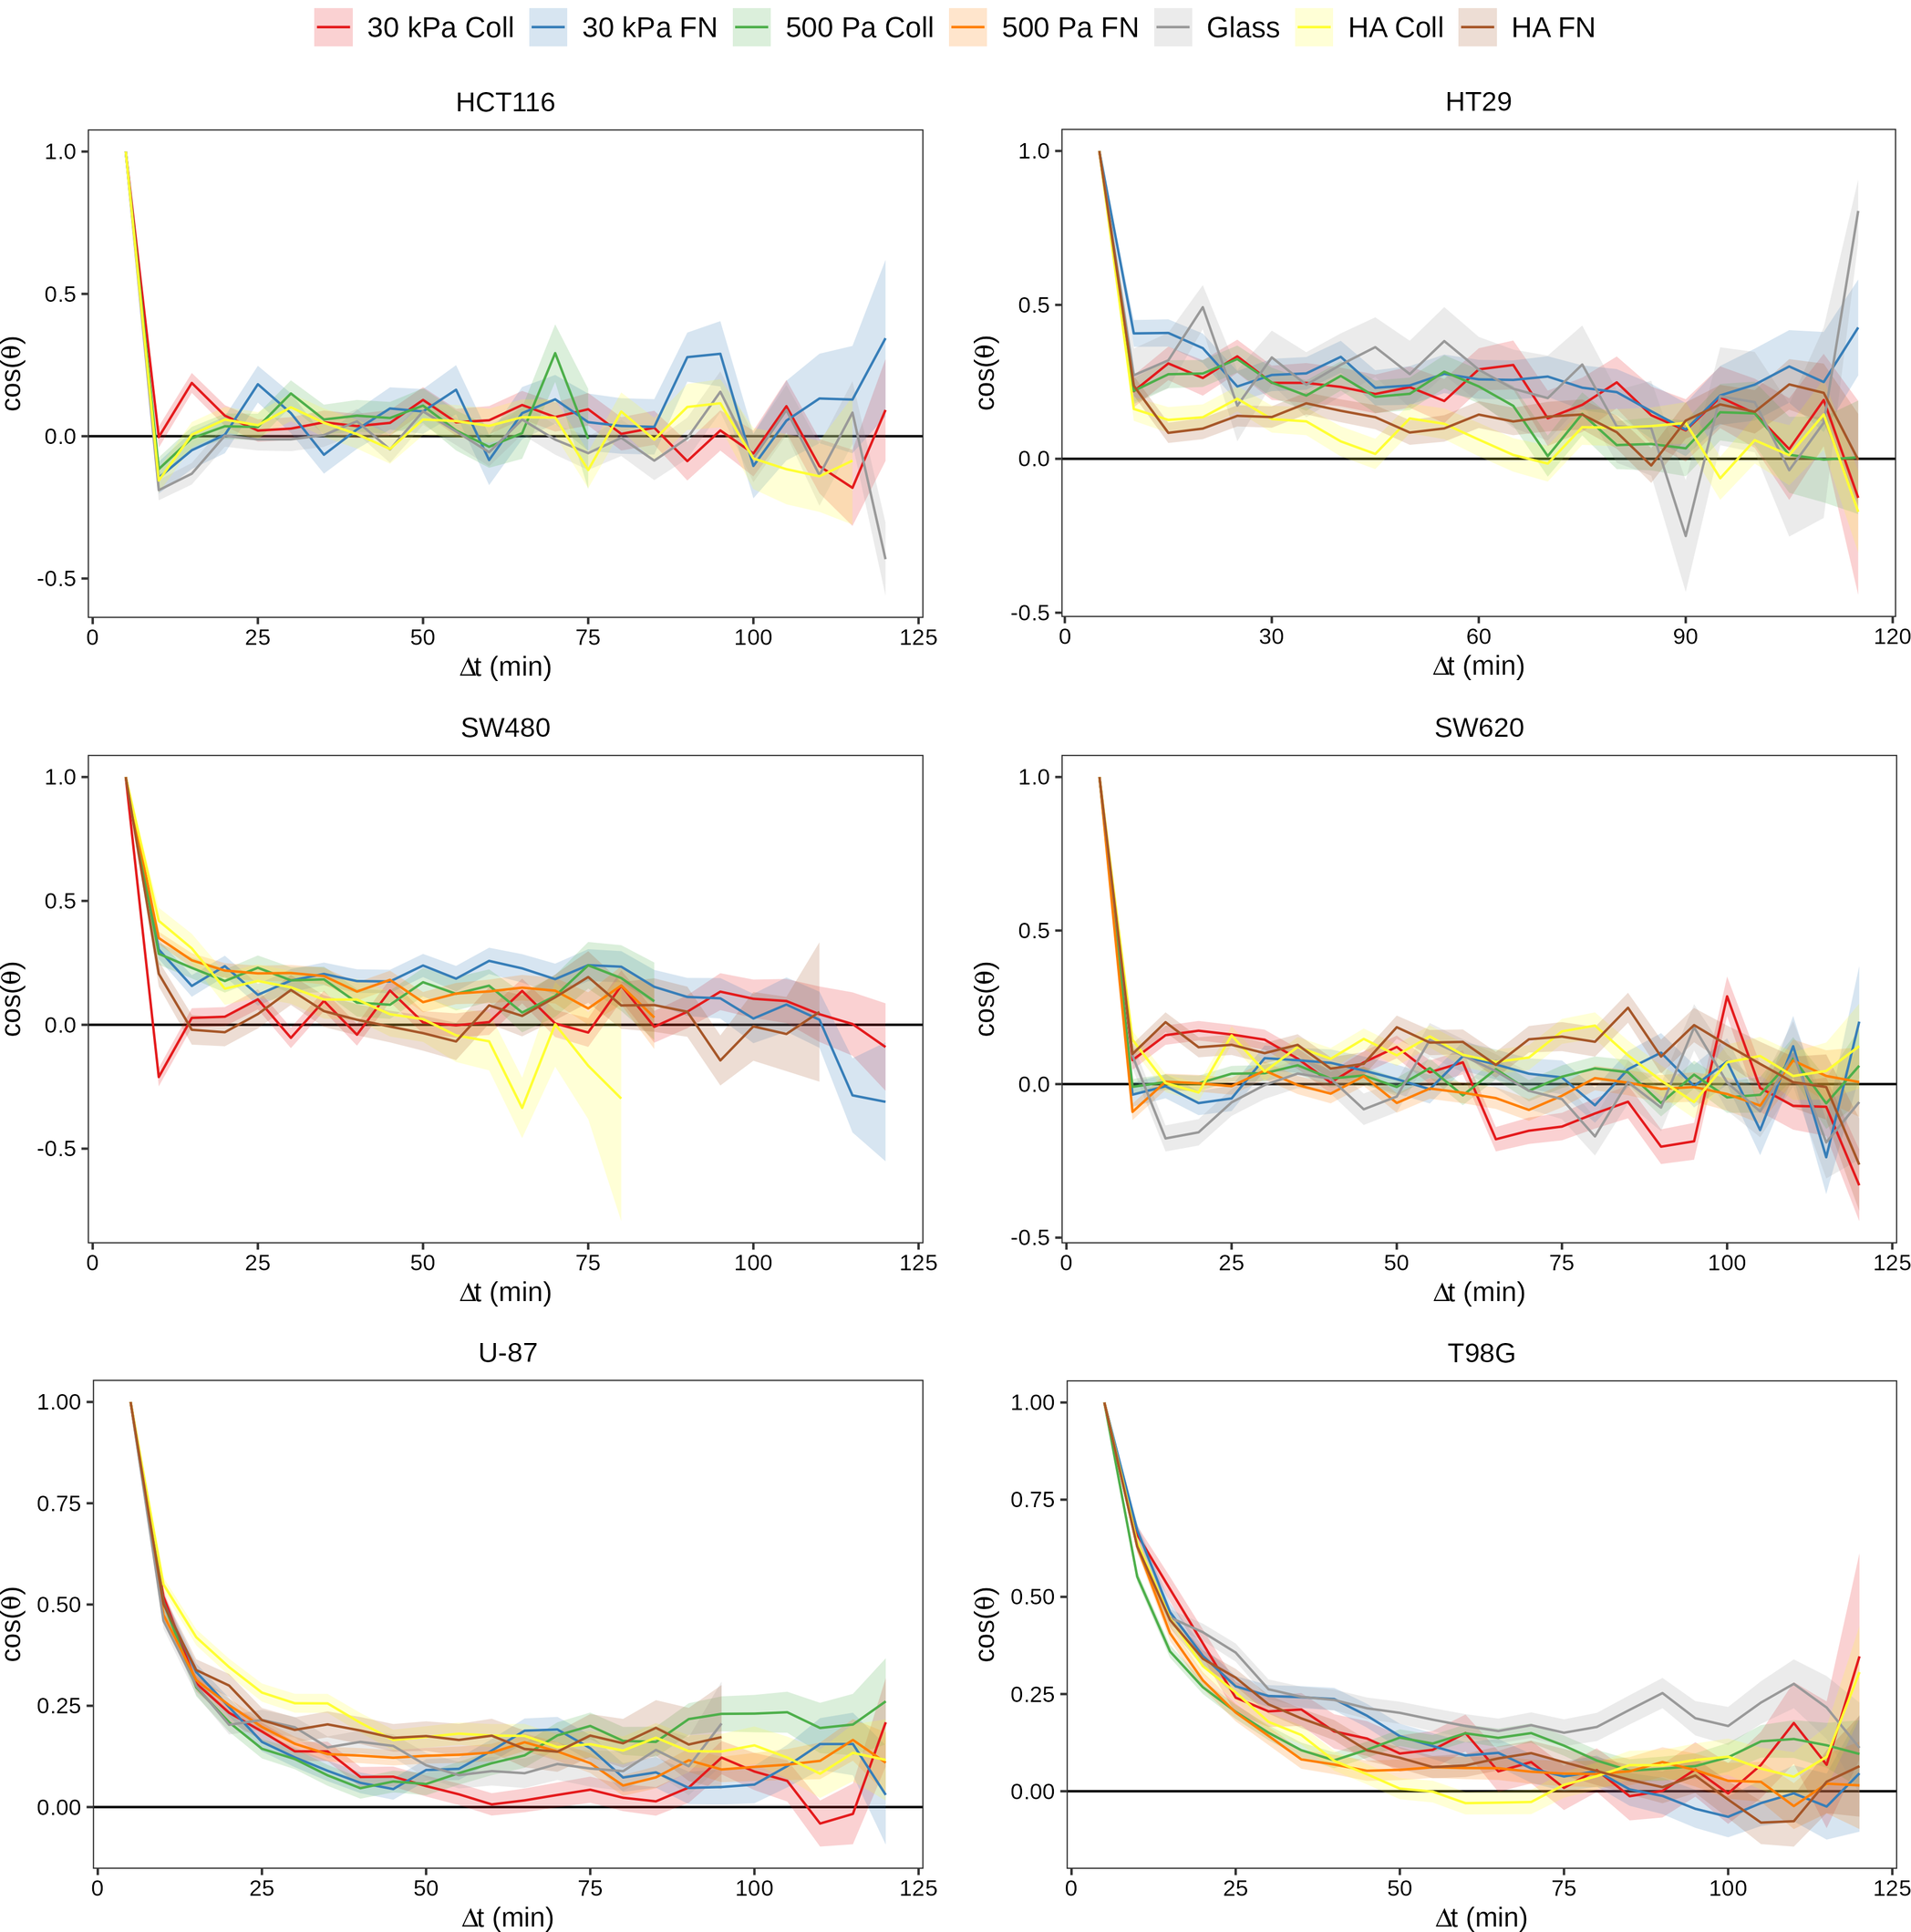
\includegraphics{../Figures/Supplementary_Figures17_21/supplementary_figure21.png}
    \caption{Directional autocorrelation comparing the persistence of cell migration for cell lines on different substrates.
    For each cell line, only those substrates are analysed that have $n \geq 25$ measurements.
    See supplementary tables 3 for the exact value of $n$ for the cell lines.}
    \label{fig:fig21}
\end{figure}

\end{document}